% ==================================================================
% Master file
% ==================================================================

\documentclass[12pt,a4paper,oneside]{scrreprt}

% ---------- Language & Encoding ----------
\usepackage{fontspec}
\defaultfontfeatures{Ligatures=TeX}
\setmainfont{Latin Modern Roman}
\setsansfont{Latin Modern Sans}
\setmonofont{Latin Modern Mono}
\usepackage[english]{babel}
\usepackage{csquotes}

\usepackage{microtype}
% Falls gewünscht: Protrusion für Text/Mathe deaktivieren
\AtBeginDocument{\microtypesetup{protrusion=false}}

% --- Unicode -> LaTeX Mappings (nur wenn Zeichen wirklich vorkommen) ---
\usepackage{newunicodechar}
\newunicodechar{′}{\ensuremath{^{\prime}}}
\newunicodechar{⇒}{\ensuremath{\Rightarrow}}
\newunicodechar{→}{\ensuremath{\to}}
\newunicodechar{≤}{\ensuremath{\le}}
\newunicodechar{≥}{\ensuremath{\ge}}

% Build-Metadaten (aus CI befüllt; lokal Fallback)
\IfFileExists{buildmeta.tex}{\input{buildmeta.tex}}{%
  \def\BuildRun{DEV}\def\BuildSHA{local}\def\BuildDate{\today}%
}

% ---------- Layout & Aesthetics ----------
\usepackage{geometry}
\geometry{
  left=3cm,right=2.5cm,top=2.5cm,bottom=3cm,
  marginparwidth=2cm,   % Platz für todonotes
  marginparsep=2mm      % Abstand zum Text
}

\usepackage{setspace}
\onehalfspacing

\newif\ifdraft
\draftfalse
\ifdraft
  \usepackage{todonotes}
\else
  \usepackage[disable]{todonotes}
\fi

% ---------- Math, Tables, Units ----------
\usepackage{amsmath,amssymb,mathtools}
\usepackage{siunitx} \sisetup{detect-all=true}
\usepackage{booktabs,array,multirow}

% ---------- Graphics ----------
\usepackage{graphicx}
\usepackage{caption}
\usepackage{subcaption}
\captionsetup{labelfont=bf}
\graphicspath{{figures/}{figures/fig/}}
% \setkeys{Gin}{draft=true} % falls Bilder fehlen

% ---------- Links & Clever refs ----------
\usepackage{xcolor}
\definecolor{linkblue}{HTML}{0A66C2}
\usepackage{hyperref}
\hypersetup{colorlinks=true,linkcolor=black,citecolor=linkblue,urlcolor=linkblue}
\usepackage[nameinlink,noabbrev]{cleveref} % nach hyperref

% Math in moving arguments (section titles, captions) -> ASCII fallback
\pdfstringdefDisableCommands{%
  \def\Cout{Cout}%
  \def\sinIn{sinIn}%
  \def\kO{kappaO}%
  \def\Theta{Theta}%
  \def\Rightarrow{=>}%
  \def\;{}%
  \def\({}%
  \def\){}%
}

% ---------- Plots (TikZ/PGF) ----------
\usepackage{pgfplots}
\pgfplotsset{compat=1.18}
\usetikzlibrary{calc,positioning}
\tikzset{every node/.style={align=center}}

% === Bibliography (biblatex+biber) with natbib compatibility ===
\usepackage[
  backend=biber,
  style=authoryear,
  sorting=nyt,
  natbib=true
]{biblatex}
\ExecuteBibliographyOptions{uniquename=init}
\addbibresource{references.bib}

% ---------- Helper Macros ----------
\usepackage{xparse}

% failsafe \addfig: bricht nicht ab, wenn Bild fehlt
\makeatletter
\@ifundefined{addfig}{%
  \NewDocumentCommand{\addfig}{O{htbp} m m m O{0.9}}{%
    \begin{figure}[#1]\centering
      \IfFileExists{\detokenize{#2}}{%
        \includegraphics[width=#5\linewidth]{\detokenize{#2}}%
      }{%
        \fbox{\parbox{.9\linewidth}{\centering Missing file:
          \texttt{\detokenize{#2}}}}%
      }%
      \caption{#3}\label{#4}
    \end{figure}}
}{%
  \RenewDocumentCommand{\addfig}{O{htbp} m m m O{0.9}}{%
    \begin{figure}[#1]\centering
      \IfFileExists{\detokenize{#2}}{%
        \includegraphics[width=#5\linewidth]{\detokenize{#2}}%
      }{%
        \fbox{\parbox{.9\linewidth}{\centering Missing file:
          \texttt{\detokenize{#2}}}}%
      }%
      \caption{#3}\label{#4}
    \end{figure}}
}
\makeatother
% --- Checklist environment (tick marks) ---
\usepackage{pifont}
\usepackage{enumitem}
\newenvironment{checklist}{%
  \begin{itemize}[label=\checkmark,leftmargin=2em]
}{%
  \end{itemize}
}


% --- Roadmap-Umgebung als Liste (Option 1b) ---
\usepackage{enumitem} % falls noch nicht vorhanden, am besten hier laden
\newenvironment{roadmap}{%
  \begin{itemize}[leftmargin=2em]
}{%
  \end{itemize}
}

% concept boxes
\newenvironment{insight}{\par\vspace{0.5em}\noindent\textbf{Insight.}\ }{\par\vspace{0.5em}}
\newenvironment{implication}{\par\vspace{0.5em}\noindent\textbf{Implication.}\ }{\par\vspace{0.5em}}
\newenvironment{limitation}{\par\vspace{0.5em}\noindent\textbf{Assumptions \\ \& Limitations.}\ }{\par\vspace{0.5em}}

% notation
\newcommand{\sinIn}{s_{\mathrm{in}}}
\newcommand{\Cout}{C_{\mathrm{out}}}
\newcommand{\kO}{\kappa_{\mathrm{O}}}

% Backward-compat für alte Font-Befehle (KOMA-safe)
\DeclareOldFontCommand{\rm}{\normalfont\rmfamily}{\mathrm}
\DeclareOldFontCommand{\sf}{\normalfont\sffamily}{\mathsf}
\DeclareOldFontCommand{\tt}{\normalfont\ttfamily}{\mathtt}
\DeclareOldFontCommand{\bf}{\normalfont\bfseries}{\mathbf}
\DeclareOldFontCommand{\it}{\normalfont\itshape}{\mathit}
\DeclareOldFontCommand{\sc}{\normalfont\scshape}{\relax}
% ==================================================================


\begin{document}
\begin{titlepage}
  \centering
  {\Large Master Thesis (Hypothesis-Driven, Physically Anchored)}\\[0.6em]
  {\huge\bfseries Roles, Thresholds, and Counting Time}\\[0.25em]
  {\Large\bfseries From Ur-Fabric to Cosmos, Life, Mind \& AI}\\[1.0em]
  {\large A Dimension-Agnostic, Falsifiable Role Calculus}\\[-0.2em]
  {\small (\,O: orientation/transport,\ G: binding/structuring,\ K:=O$\!\circ$G;\ $t:=C[\tau^K]$\,)}\\[2.0em]

  \begin{tabular}{@{}ll@{}}
    Author: & Tim Brötzmann \\
    Submission date: & \today \\
    Build: & Run \BuildRun\ (\BuildSHA) — \BuildDate \\
  \end{tabular}

  \vfill
  \IfFileExists{figures/logo-placeholder}{\includegraphics[width=0.28\linewidth]{figures/logo-placeholder}}{}
\end{titlepage}

\pagenumbering{roman}

\chapter*{Abstract}
We propose a dimension-agnostic \emph{role calculus} in which two primitives—
\emph{orientation/transport} $O$ and \emph{binding/structuring} $G$—generate 
observable structure. A non-acting reader $C$ counts events, so that time is not 
a force but an order parameter: $\tau^O$ counts $O$-events, $\tau^K$ counts 
composite overlap events $K:=O\!\circ G$, and macroscopic time continues as 
$t:=C[\tau^K]$. No new forces are introduced; sector avatars (gravity, electrostatics, 
radiation, networks) appear as weak-field realizations of the same roles.

Dynamics are organized by two thresholds: a \emph{seed} threshold $\Theta$ 
(local nucleation) and a \emph{persistence} threshold $\sigma_c$ (long-lived 
channels). This yields three falsifiable, parameter-light signatures: 
\emph{T1} (orientation law: $+1/-2$ slopes with parameter-free inside--outside 
identity, generalizable to $D$ dimensions); 
\emph{T2} (bridge law: finite cross-coherence band $0<C_1(k)<1$ removable 
by null tests); 
\emph{T3} (threshold law: nucleation--persistence hysteresis with loop area 
$\mathcal A_{\rm loop}>0$).

The same roles map across scales—Ur-fabric $\rightarrow$ cosmos $\rightarrow$ 
molecules $\rightarrow$ life $\rightarrow$ mind/AI. This framework resonates with 
universality principles in physics (Kadanoff, Wilson), error thresholds in molecular 
evolution (Eigen; Szathmáry \& Maynard Smith), and systemic coherence theories 
in neuroscience (Tononi’s IIT; Friston’s Free Energy Principle). Unlike 
domain-specific models, it enforces a minimal and falsifiable calculus: 
cross-scale invariants (slopes, coherence windows, hysteresis loops) provide 
operational tests while remaining compatible with higher-$D$ hypotheses.

\chapter*{Keywords}
role calculus; orientation $O$; binding $G$; composition $K{:=}O\!\circ G$; 
counting time $t{:=}C[\tau^K]$; thresholds $\Theta,\sigma_c$; hysteresis; 
cross-coherence $C_1(k)$; universality; falsifiability; black-hole release shell; 
error threshold; coordination plateaus (C$_2$); universality-class stance; 
dimension-agnostic.

\pagenumbering{roman}       % kleine römische Zahlen
\tableofcontents
\listoffigures
\listoftables

\clearpage
\pagenumbering{arabic}  

\part{Introduction}

\section*{Plain-language overview}
This work asks a simple question with far-reaching consequences: 
\emph{Are two roles enough to organize what we see across physics, biology, and cognition?} 
We call them \textbf{orientation/transport} ($O$) and \textbf{binding/structuring} ($G$). 
They are not new forces but rather \emph{what processes do}. 
A reader $C$ makes these roles visible and \emph{counts}: $\tau^O$ counts $O$-events; 
$\tau^K$ counts overlap-events $K := O \!\circ G$; macroscopic time is the coarse continuation $t := C[\tau^K]$. 
From this vantage point, familiar patterns---inverse-square laws, potential wells, flows, membranes, neurons, or even markets---look like \emph{the same grammar} recurring at different scales.

What is genuinely new here is not a metaphysical claim but a \emph{testable} one. 
In weak fields, stacks around approximately spherical deficits must show a paired slope signature $(+1,-2)$ and a parameter-free inside--outside identity. 
Flows and potentials should only partially align (a finite $0<C_1(k)<1$ band), and thresholded systems should exhibit nucleation--persistence hysteresis. 
These three signatures (T1--T3) are our through-line from Ur-fabric to cosmos, life, mind, and AI.

\subsection*{What is new here (in one page)}
\begin{enumerate}
  \item \textbf{Counting time.} Time is operationalized as counting of real events: $\tau^O$, $\tau^K$, and $t = C[\tau^K]$. $C$ \emph{does not act}; it reads. 
  This connects to the idea of time as an order parameter in statistical physics.
  \item \textbf{Dimension-agnostic weak-field law.} The orientation avatar yields inner/outer slopes and a parameter-free identity. 
  In 3D this is $(+1,-2)$ with $C_{\mathrm{out}}/s_{\mathrm{in}}=a^3$; in $D$ dimensions it generalizes to $(+1,-(D{-}1))$ and $a^{D}$.
  \item \textbf{Cross-coherence bridge.} Flows vs.\ potentials exhibit a finite coherence band $0<C_1(k)<1$---\emph{not} a perfect lock---organizing residuals and scale-coupling. 
  This resonates with cross-scale correlations in critical phenomena \citep{Wilson1971RG,Kadanoff1966}.
  \item \textbf{Thresholds and hysteresis.} Two thresholds matter: a seed threshold $\Theta$ (nucleation) and a persistence threshold $\sigma_c$ (long-lived channels). 
  Their operational face is a hysteresis loop with area $\mathcal A_{\rm loop}>0$, paralleling Eigen's \emph{error threshold} in evolutionary dynamics \citep{Eigen1971,Szathmary1995}.
  \item \textbf{Same roles across layers.} Ur-fabric $\to$ cosmos (e.g.\ near-horizon “release shells”), $\to$ molecules \& life (Keim window, compartments), $\to$ mind/AI (coordination plateaus, apex keim). 
  No new primitives are added; only avatars and parameters change. 
  This parallels universality classes in physics, where different micro-dynamics collapse into shared critical exponents.
\end{enumerate}

\subsection*{Key questions}
\begin{enumerate}
  \item \emph{Minimality.} Are $O$ and $G$ sufficient as role primitives once time is treated as counting via $C$?
  \item \emph{Falsifiability.} Do data exhibit T1 (paired slopes $+1/-2$ and identity), T2 (finite $C_1(k)$ band with null removal), and T3 (hysteresis with $\mathcal A_{\rm loop}>0$)?
  \item \emph{Bridging.} Can the same tests diagnose overlap events from Ur-fabric to black-hole environs, to prebiotic chemistry, to neural coordination? 
  This echoes the search for cross-scale invariants in biology (Eigen's thresholds) and neuroscience (Tononi’s IIT, Friston’s Free Energy Principle \citep{Tononi2004IIT,Friston2010FEP}).
  \item \emph{Robustness.} Do results hold in strict $3{+}1$D---and how would higher-$D$ hypotheses show up (exponent/coupling shifts) without adding new primitives?
\end{enumerate}

\begin{insight}
\textbf{Role vs.\ mechanism.} We separate \emph{what} a process does ($O,G$) from \emph{how} it is implemented (microphysics). 
This keeps the language compact across domains and puts tests first.
\end{insight}

\begin{implication}
\textbf{One toolkit, many layers.} If the role signatures persist, we gain a common diagnostic and reporting standard---from gravity avatars to protocells to coordinated neural plateaus. 
This suggests a universality-class stance that spans physics, life, and cognition.
\end{implication}

\begin{limitation}
\textbf{Not a replacement for microphysics.} The role calculus constrains sector models via cross-scale regularities; it must \emph{earn} value by identities that survive measurement and null tests.
\end{limitation}

\paragraph{Methodological stance (diagnostics, not forces).}
Throughout this work, $O$ (guidance), $G$ (binding), and $C$ (counting) are treated as 
\emph{diagnostic primitives}. They provide a measurement calculus for thresholds, windows, 
and overlaps, but they do not introduce new forces or ontological entities. 
All claims are operational: coherence measures and threshold signatures 
(e.g.\ $C_1$, $C_2$, hysteresis loops) are read as \emph{diagnostic summaries}, 
not as causal dynamics in themselves \cite{friston2006free, bollobas1998random}.
This stance ensures that results remain falsifiable and transferable across 
domains (physics, chemistry, biology, human systems, AI).

\subsection*{What we will test (map for the reader)}
\textbf{T1 Orientation (weak-field)}: $(+1,-2)$ slopes and $C_{\mathrm{out}}/s_{\mathrm{in}}=a^3$ (with $a^{D}$ generalization).\\
\textbf{T2 Bridge (cross-coherence)}: finite $0<C_1(k)<1$ band, removed by phase-shuffle nulls.\\
\textbf{T3 Thresholds (hysteresis)}: distinct on/off thresholds $(\Theta_\uparrow,\Theta_\downarrow)$ with loop area $\mathcal A_{\rm loop}>0$.\\[0.3em]
\emph{Context-specific hooks (later sections).} 
BH “tree’’ (B-tests: echoes, extra $C_1(k)$ near the photon ring, HFQPO over-ISCO); 
life “Keim window’’ ($\Delta\mu_{\rm eff}\gtrsim \Theta_{\rm eff}$), viability bound $\varepsilon_{\rm req}$, error threshold $Q^L s>1$, compartment retention; 
coordination plateaus (C$_2$) for mind/AI and apex keim with guardrails.

\part{Ur-Fabric: Core Calculus and Predictions}\label{part:ur}

\chapter{Triad, Primitive Roles, and Counting Time}\label{ch:ur-triad}

\section{Purpose and stance}\label{sec:ur-purpose}

\begin{insight}
\textbf{What we build.} 
We develop a compact \emph{role calculus} based on two primitives—
\emph{orientation/transport} ($O$) and \emph{binding/structuring} ($G$)—
together with a non-acting reader $C$. 
The reader does not generate dynamics but only \emph{makes roles visible and counts}: 
$\tau^O$ counts $O$-events; $\tau^K$ counts overlap-events $K := O \!\circ G$; 
macroscopic time is the coarse continuation $t := C[\tau^K]$. 
This definition frames time as an \emph{order parameter} rather than a fundamental force, 
echoing treatments of time in statistical mechanics and dynamical systems.
\end{insight}

\begin{implication}
\textbf{Why roles (not new forces).} 
If diverse domains---gravity, electrostatics, radiation, networks, biology---share the same few 
\emph{role signatures}, then a single grammar can be tested across scales with parameter-light criteria. 
This stance resonates with universality classes in physics, where very different microscopic 
interactions collapse into shared scaling laws near critical points \citep{Wilson1971RG,Kadanoff1966}. 
Here, instead of introducing new entities, we emphasize the sufficiency of $O$ and $G$ as cross-domain roles.
\end{implication}

\begin{limitation}
\textbf{Scope.} 
The calculus \emph{does not} replace microphysics. 
It constrains existing models via cross-scale regularities that must survive 
measurement and null tests. 
Its value must therefore be \emph{earned} by falsifiable identities---analogous 
to how Eigen's error threshold sets strict viability bounds in evolutionary models 
\citep{Eigen1971,Szathmary1995}.
\end{limitation}

\begin{figure}[ht]
\centering
\begin{tikzpicture}[node distance=2.5cm,>=stealth,thick]

% Triad nodes
\node[circle,draw,minimum size=1.2cm] (N) {N};
\node[circle,draw,minimum size=1.2cm,right=of N] (S) {S};
\node[circle,draw,minimum size=1.2cm,above=1.5cm of $(N)!0.5!(S)$] (C) {C};

% Roles
\node[minimum width=2.2cm, align=center] (O) {Orientation\\($O=C\circ N$)};

% Counting time

% Mittelpunkt zwischen O und G als (leere) Referenz-Node
\begin{tikzpicture}
  % 1) Erst die Referenz-Nodes definieren
  \node (O) [circle,draw,minimum size=8mm] {O};
  \node (G) [circle,draw,minimum size=8mm, right=4cm of O] {G};

  % 2) Mittelpunkt einmal als leere Node/Koordinate anlegen
  \node (OGmid) at ($(O)!0.5!(G)$) {};

  % 3) Jetzt relativ dazu platzieren (hier: 2.5cm darunter)
  \node[rectangle,draw,rounded corners,
        minimum width=4cm, align=center,
        below=2.5cm of OGmid] (Time)
        {Counting Time\\ $\tau^O,\,\tau^K,\, t=C[\tau^K]$};
\end{tikzpicture}

% Emergence
\node[rectangle,draw,rounded corners,
      below=2.5cm of Time,
      minimum width=6cm,
      align=center] % <-- wichtig für \\ im Node
      (Emerg)
      {Avatars across scales:\\
       Cosmos $\rightarrow$ Molecules $\rightarrow$ Life $\rightarrow$ Mind/AI};

% Arrows from triad to C
\draw[->] (N) -- (O);
\draw[->] (S) -- (G);
\draw[->] (C) -- (O);
\draw[->] (C) -- (G);

% From O,G to Time
\draw[->] (O) -- (Time);
\draw[->] (G) -- (Time);

% From Time to Emergence
\draw[->] (Time) -- (Emerg);

% Labels
\node[above left=0.1cm of O] (lO) {};
\node[above right=0.1cm of G] (lG) {};

\end{tikzpicture}
\caption{Schematic of the Ur-fabric triad. Consciousness ($C$) acts diagnostically on absence ($N$) and presence ($S$) to yield two primitive roles: orientation ($O$) and binding ($G$). Time emerges by counting role events, and higher layers appear as effective avatars across scales.}
\label{fig:ur-fabric-triad}
\end{figure}

\section{Assumptions and notation}\label{sec:ur-assumptions}

\paragraph{Weak-field assumptions.} 
We adopt three standard assumptions in the weak-field regime:  
(A1) \emph{Locality} --- interactions are mediated through fields whose effects depend only on arbitrarily small neighborhoods of a point.  
(A2) \emph{Isotropy} --- in the absence of structured sources, diagnostics are rotationally invariant on average, with deviations vanishing in large, balanced stacks.  
(A3) \emph{Linear superposition} --- responses add linearly for weak fields; nonlinearities are admitted as higher-order corrections but must vanish under down-scaling (a renormalization constraint \citep{Wilson1971RG,Kadanoff1966}).  

\paragraph{Basis.} 
The substrate is expressed as a contrast $(S,N)$ between presence ($S$) and absence ($N$). 
Role primitives emerge via diagnostic self-reference: 
$O = C \circ N$ (orientation/transport) and $G = C \circ S$ (binding/structuring).  

\paragraph{Diagnostics.} 
We distinguish three diagnostic levels:  
$C_0$ --- \emph{systemic coherence}, a non-operative gauge of organization (range $0$–$1$).  
$C_1(k)$ --- \emph{cross-coherence} between flows and potentials, serving as a bridge variable.  
$C_2$ --- \emph{coordination coherence}, used for life- and mind-level processes (e.g.\ neural plateaus, collective AI states).  
These diagnostics parallel measures of coherence used in neuroscience and complexity theory, such as Tononi’s integrated information $\Phi$ \citep{Tononi2004IIT} and Friston’s free-energy minimization frameworks \citep{Friston2010FEP}.

\paragraph{Role intensity.} 
A convenient role intensity is defined as
\begin{equation}
\sigma(O,G) = \alpha \|O\|^2 - \beta \|G\|^2, 
\qquad \alpha,\beta>0,
\end{equation}
capturing the balance between orientation and binding contributions. 
Critical values of $\sigma$ will seed thresholds and hysteresis (see Sec.~\ref{sec:thresholds}).

\paragraph{Moderate universality (Assumption U).} 
$O$ and $G$ are primitive on the Ur-fabric. 
Higher layers (cosmos, chemistry/life, human/AI) deploy effective \emph{avatars} $O_{\mathrm{eff}}, G_{\mathrm{eff}}$ that preserve algebraic roles (Gauss-type counting, gradient vs.\ potential structures). 
While curls, anisotropies, or nonlinear corrections may appear at higher levels, they must vanish in the weak-field limit. 
This stance reflects a universality-class view: different microphysics can collapse into the same effective role behavior, analogous to shared exponents in critical phenomena \citep{Wilson1971RG}. 

\section{Phase, superposition, and reading}\label{sec:ur-phase}

Before the reader $C$ registers events, role-states can exist in coherent superpositions over $(S,N)$:
\[
\lvert \psi \rangle 
= \cos\frac{\theta}{2}\lvert N \rangle 
+ e^{i\phi}\sin\frac{\theta}{2}\lvert S \rangle.
\]
Here, $\phi$ controls interference between absence and presence. 
The act of reading by $C$ projects the state to real counts ($0/1$ outcomes), thereby accruing $\tau^O$ and $\tau^K$. 

\paragraph{Geometric compression of phase.} 
Geometry can \emph{compress phase}, providing guidance or structural support that lengthens coherence times. 
When coherence is maintained long enough, a threshold-crossing event can occur ($\Delta\tau^K = 1$). 
Otherwise, decoherence dominates and no new counts accrue. 
This echoes how geometric or boundary conditions in quantum and condensed-matter systems extend coherence lifetimes by suppressing environmental noise \citep{Zurek2003Decoherence}.

\paragraph{Conceptual role.} 
Phase thus acts as a preparatory layer: a latent resource that can be harvested into discrete events by $C$. 
This perspective connects role calculus to established ideas of \emph{superposition and measurement} in quantum theory, while remaining general enough to apply to biological and cognitive domains. 
For example, coherence compression resembles mechanisms in protein folding landscapes or neural synchrony, where geometry and connectivity shape the stability of phase relationships \citep{Tegmark2000Importance,Friston2010FEP}.

\paragraph{Diagnostic implication.} 
Phase-compression events correspond to moments where latent coherence is converted into countable thresholds. 
Such transitions can be probed experimentally: in physics (ringdown echoes near black holes), in chemistry (transition-state stabilization in catalysis), or in neuroscience (extended synchrony in EEG/MEG plateaus). 
Across these domains, the reader $C$ remains diagnostic: it registers but does not act, ensuring that coherence is translated into empirical counts rather than assumed forces.

\section{Primitive process forms}\label{sec:ur-primitives}

\paragraph{Diagnostic definition.} 
At the most compact level, role primitives are defined as
\begin{equation}
O := C_0 \!\circ N \quad \text{(orientation/transport)}, 
\qquad
G := C_0 \!\circ S \quad \text{(binding/structuring)}, 
\qquad
K := O \!\circ G \ \ \text{(overlap; non-commutative)}.
\end{equation}
Here, $C_0$ denotes a systemic, non-operative diagnostic. 
$O$ captures the role of orientation (movement, gradients, counting flux), 
$G$ the role of binding (cohesion, potential wells, structure), 
and $K$ their overlap composition, encoding interactions where transport and binding meet. 

\paragraph{Counting clocks.} 
Time is expressed as a hierarchy of counts: 
\[
\tau^O = \operatorname{ord}\{O_k\}, \quad 
\tau^K = \operatorname{ord}\{K_k\}, \quad 
t = C[\tau^K].
\]
This formulation stresses that time is \emph{read} rather than imposed: 
the act of counting by $C$ transforms latent role interactions into macroscopic order. 
This resonates with information-theoretic views of time as emergent from event orderings 
rather than as a primitive background \citep{Rovelli1995Time}.

\paragraph{Conceptual role.} 
These primitives provide a basis for higher-layer avatars. 
In physics, $O$ resembles divergence-type counting in Gauss laws, 
while $G$ parallels gradient accumulation in potential theory. 
In biology, $O$ can be read as flows of metabolites or genetic information, 
while $G$ represents structural binding in membranes or genomes. 
Their overlap $K$ encodes non-commutative couplings, akin to catalytic sites in chemistry 
or synchronized binding–release cycles in molecular motors. 
The non-commutativity of $K$ is essential: order matters when transport and binding interact, 
a property shared by many complex systems from turbulence to neural coordination \citep{Laughlin2000Emergent}.

\paragraph{Cross-domain analogy.} 
This minimal role grammar aims to formalize what process philosophers such as Whitehead described informally: 
that becoming precedes being, and that recurrent patterns of orientation and binding structure the flow of existence \citep{Whitehead1929Process}. 
Here, however, these ideas are sharpened into falsifiable process forms, equipped with counts and thresholds.

% Optional schematic
\begin{figure}[ht]
\centering
\begin{tikzpicture}[node distance=3cm,>=stealth,thick]
\node[rectangle,draw,rounded corners,minimum width=2.8cm,minimum height=1cm] (N) {Absence $N$};
\node[rectangle,draw,rounded corners,minimum width=2.8cm,minimum height=1cm,right=of N] (S) {Presence $S$};
\node[circle,draw,above=1.5cm of $(N)!0.5!(S)$,minimum size=1.2cm] (C0) {$C_0$};

\node[rectangle,draw,rounded corners,below left=1.5cm of N,minimum width=2.8cm] (O) {$O=C_0\!\circ N$ \\ Orientation/Transport};
\node[rectangle,draw,rounded corners,below right=1.5cm of S,minimum width=2.8cm] (G) {$G=C_0\!\circ S$ \\ Binding/Structuring};

\node[rectangle,draw,rounded corners,below=3cm of $(O)!0.5!(G)$,minimum width=5.5cm] (K) {$K=O\!\circ G$ \\ Overlap (non-commutative)};

\draw[->] (C0) -- (O);
\draw[->] (C0) -- (G);
\draw[->] (N) -- (O);
\draw[->] (S) -- (G);
\draw[->] (O) -- (K);
\draw[->] (G) -- (K);

\end{tikzpicture}
\caption{Primitive process forms. Orientation ($O$) arises from diagnostic reading of absence ($N$), 
binding ($G$) from presence ($S$). Their non-commutative overlap $K$ encodes coupled processes.}
\label{fig:primitive-forms}
\end{figure}

\section*{Roadmap: Why $O,G,K$ matter}
\begin{insight}
\textbf{Fundamental stance.} 
Orientation ($O$) and binding ($G$) are taken as role primitives, 
with their overlap ($K$) encoding interactions. 
Time is not introduced as an external parameter but emerges from counting 
of $K$-events by $C$. 
This minimal set is sufficient to express dynamics across scales.
\end{insight}

\begin{implication}
\textbf{Cross-domain signatures.} 
Because $O,G,K$ preserve their algebraic form, they generate testable 
signatures that appear in physics (inverse-power flows, Gauss identities), 
in chemistry/biology (thresholds, error bounds), and in cognition/AI 
(coherence plateaus). 
Universality principles \citep{Wilson1971RG} suggest that very different 
systems can share the same effective exponents, supporting this stance.
\end{implication}

\begin{limitation}
\textbf{Tests before claims.} 
The framework does not assert new forces or hidden substances. 
Its scientific value must be earned by \emph{tests}:  
slope-pairs (T1), finite cross-coherence bands (T2), and hysteresis loops (T3). 
Only if these invariants hold across scales does the calculus gain legitimacy.
\end{limitation}

\section{Minimal orientation avatar (weak-field, \(D\) spatial dimensions)}\label{sec:ur-orientation}

We now specify the orientation role $O$ in the weak-field limit. 
Let the orientation field be irrotational,
\begin{align}
\mathbf v_O &= \kappa_O \nabla \Omega, && \text{(O1)}\\
\nabla \!\cdot \mathbf v_O &= S_D \, \kappa_O \, \rho_N 
\ \Longleftrightarrow\ \ \nabla^2 \Omega = S_D \, \kappa_O \, \rho_N, && \text{(O2)}
\end{align}
where $\rho_N$ denotes deficit density and $S_D$ is the $D$-sphere surface factor 
($S_3 = 4\pi$). 
For a point source $n$, the potential and radial flow follow:
\begin{equation}
\Omega(r) = -\frac{\kappa_O n}{r^{D-2}}, 
\qquad 
\mathbf v_O(r) = \frac{\kappa_O n}{r^{D-1}} \, \mathbf e_r. 
\quad \text{(O3)}
\end{equation}

\paragraph{Interpretation.} 
Equation (O3) shows that the orientation avatar reproduces the familiar 
inverse-square law in three dimensions ($D=3$). 
In higher dimensions, the slope generalizes naturally to $(+1, -(D{-}1))$, 
providing a simple dimensional diagnostic: geometry fixes the exponents without 
introducing new primitives. 
The constant $\kappa_O$ plays the role of an orientation coupling, fixed once 
by Gauss-type counting and not adjustable sector by sector.

\paragraph{Conceptual role.} 
This formulation highlights the minimal stance: the same algebraic structure 
generates gravitational-type and electrostatic-type avatars as weak-field 
limits of orientation. 
What appears as Newton’s $1/r^2$ law or Coulomb’s law is here read as a 
parameter-free role identity, not a separate postulate. 
In this sense, $O$ captures the universality of inverse-power scaling 
seen in multiple domains, echoing renormalization insights that 
different microphysics can collapse into the same effective exponents 
\citep{Wilson1971RG}.

\paragraph{Cross-scale analogy.} 
Orientation signatures are not restricted to physics. 
In biology, diffusion fluxes also follow inverse-power decays, 
and in neural fields, long-range coherence often exhibits 
power-law attenuation with distance. 
The role avatar $O$ thus acts as a unifying diagnostic: 
a minimal law appearing whenever orientation processes dominate 
over binding or nonlinear corrections.

\section{Geometric signatures around spherical deficits}\label{sec:ur-signatures}

Consider a homogeneous core of radius $a$. 
The radial slope index is
\begin{align}
\beta_O(r) &:= \frac{d\ln v_r}{d\ln r} 
= \begin{cases}
+1, & r \le a, \\
-(D-1), & r \ge a,
\end{cases} \label{eq:slopesD} \\
\frac{C_{\rm out}}{s_{\rm in}} &= a^{D}, \qquad 
C_{\rm out} := r^{D-1} v_r \big|_{r \ge a}, \quad
s_{\rm in} := \frac{dv_r}{dr}\bigg|_{r \le a}.
\label{eq:identityD}
\end{align}
In three spatial dimensions, Eq.~\eqref{eq:slopesD} reduces to the familiar $(+1,-2)$ slope pair, 
and Eq.~\eqref{eq:identityD} yields the parameter-free identity $C_{\rm out}/s_{\rm in} = a^3$.

\begin{implication}
\textbf{Parameter-free test (T1).} 
Stacks that fail to exhibit the $(+1,-2)$ slopes and the inside--outside identity falsify 
the weak-field orientation law. 
A systematic slope shift from $-2$ to $-(D-1)$ would serve as a diagnostic for effective 
higher-dimensional behavior, without invoking new primitives.
\end{implication}

\paragraph{Interpretation.} 
The $(+1,-2)$ law is remarkable because it does not rely on adjustable parameters: 
geometry alone enforces it. 
This makes the test falsifiable in the Popperian sense: a single robust counterexample 
would invalidate the role calculus at this level. 
Such parameter-free predictions are rare and valuable, as they allow strong comparisons 
with observational data (e.g.\ gravitational lensing slopes, electrostatic field fall-offs). 

\paragraph{Conceptual role.} 
These slope identities express how orientation processes self-balance around 
deficits. The inner region ($+1$) represents coherent transport filling in the deficit, 
while the outer region ($-2$ in 3D) describes dispersal governed by surface geometry. 
This duality resonates with universal scaling behavior seen in renormalization theory, 
where slopes and exponents act as invariants across otherwise diverse systems 
\citep{Wilson1971RG,Kadanoff1966}. 

\paragraph{Cross-scale analogy.} 
Beyond physics, similar slope breaks occur in biological and cognitive systems: 
nutrient uptake curves often show an inner linear regime and an outer diminishing-return falloff, 
while neural synchrony frequently decays with distance according to power-law exponents. 
The $(+1,-2)$ signature is thus interpreted not as a quirk of gravitation, 
but as a universal diagnostic of orientation roles across scales.

\section*{Roadmap: Orientation test (T1)}
\begin{insight}
\textbf{Why it matters.} 
The slope law $(+1,-2)$ is the first concrete, parameter-free diagnostic 
of the role calculus. 
It turns an abstract primitive ($O$) into a falsifiable prediction.
\end{insight}

\begin{implication}
\textbf{What it enables.} 
By comparing observed slope pairs in physics (fields), chemistry (diffusion fronts), 
and cognition (coherence decay), we obtain a universal benchmark. 
A verified slope-shift from $-2$ to $-(D-1)$ would even diagnose 
effective higher-dimensional behavior. 
\end{implication}

\begin{limitation}
\textbf{What it is not.} 
The slope identity is not a model of microphysics. 
It constrains models: any sector law that fails this simple geometric test 
cannot be reconciled with the calculus.
\end{limitation}


\section{Direct determination of the orientation coupling}\label{sec:ur-kappa}

If sources are countable, the orientation coupling $\kappa_O$ can be determined directly from either 
exterior or interior diagnostics:
\begin{equation}
\kappa_O = \frac{C_{\rm out}}{N} 
= \frac{r^{D-1} v_r}{S_D \, a^{D} \rho_N} \quad (r \ge a),
\qquad 
\kappa_O = \frac{1}{S_D} \, \frac{s_{\rm in}}{\rho_N} \quad (r \le a).
\end{equation}
Consistency requires that interior and exterior estimates agree within experimental or 
observational uncertainties, across environments and scales. 

\paragraph{Interpretation.} 
This relation highlights that $\kappa_O$ is not a free parameter but a 
count-derived constant. 
Once fixed in one context, it must apply universally: the same $\kappa_O$ 
should govern gravitational-like and electrostatic-like avatars, as well as 
diffusion-type processes in biological or network systems. 
This provides a stringent falsifiability condition: if different environments 
yield incompatible values of $\kappa_O$, the role calculus is refuted at this level. 

\paragraph{Conceptual role.} 
The orientation coupling acts as the \emph{universal scale factor} translating 
between source counts ($N$, $\rho_N$) and observed fluxes ($v_r$). 
In physics this parallels how Gauss’s law fixes the proportionality between 
charge and field, or mass and gravitational acceleration \citep{Jackson1999Classical}. 
In biology, an analogous role is played by uptake rates normalized by nutrient 
sources; in neuroscience, by coherence measures normalized to underlying 
signal counts. 
In each case, the demand that interior and exterior measures agree functions as 
a conservation law for orientation processes. 

\paragraph{Cross-scale implication.} 
Because $\kappa_O$ is fixed by count identities rather than tunable constants, 
it offers a robust diagnostic for testing universality across domains. 
A breakdown would signal either measurement error or the need for new primitives. 
Thus, $\kappa_O$ stands as a bridge between micro-level counts and macro-level 
fluxes, reinforcing the minimality stance of the calculus.

\section{Thresholds: seed vs.\ persistence}\label{sec:ur-thresholds}

Two thresholds organize dynamics in the role calculus: 
\begin{align}
\sigma(O,G) &\ge \Theta 
\ \Rightarrow\ \text{nucleation (stable pair or excitation)}, \\
\sigma(O,G) &\ge \sigma_c > \Theta 
\ \Rightarrow\ 
\begin{cases}
\text{$G$-dominated channel } \to \text{bound contents (``matter'')}, \\
\text{$O$-dominated channel } \to \text{transport contents (``energy'')}.
\end{cases}
\end{align}

\paragraph{Seed vs.\ persistence.} 
The \emph{seed threshold} $\Theta$ marks the minimum intensity required for 
local nucleation---the first appearance of a stable pair or excitation. 
Crossing the higher \emph{persistence threshold} $\sigma_c$ ensures that 
channels become long-lived, separating into $G$-dominated (binding/matter-like) 
and $O$-dominated (transport/energy-like) pathways. 

\paragraph{Hysteresis.} 
Because feedback between guided transport and consolidation 
is not symmetric, nucleation and extinction thresholds differ: 
\[
(\Theta_\uparrow, \Theta_\downarrow), \qquad 
\mathcal A_{\rm loop} > 0.
\]
This hysteresis loop provides a direct operational signature (T3). 
Reporting loop area and asymmetry is essential for empirical testing. 

\paragraph{Conceptual role.} 
Thresholds act as \emph{bifurcation points}: once crossed, systems qualitatively 
change their mode of behavior. 
In statistical physics, such bifurcations appear in phase transitions 
and critical phenomena \citep{Stanley1971Phase}. 
In evolutionary biology, Eigen’s \emph{error threshold} marks a similar 
boundary between viable and collapsing quasispecies \citep{Eigen1971,Szathmary1995}. 
In neuroscience, hysteresis is a hallmark of multi-stable coordination states, 
from perceptual switches to neural synchrony plateaus \citep{Kelso1995Coordination}. 

\paragraph{Cross-scale implication.} 
This dual-threshold logic provides a unifying grammar: 
from nucleation of matter near black holes (release shells), 
to the viability of protocells (Keim window, error thresholds), 
to the coordination plateaus in neural or AI systems. 
In each case, the calculus predicts that crossing persistence thresholds 
is accompanied by measurable hysteresis, providing a robust falsifiability 
criterion across domains.

\section{Transport and circulation families}\label{sec:ur-families}

\paragraph{Source-free transport.} 
A scalar payload $q$ advects on orientation streamlines:
\[
\partial_{\tau} q + \nabla \!\cdot (q\, \mathbf v_O) = 0, 
\qquad \mathbf v_O = \kappa_O \nabla \Omega.
\]
This represents pure transport without sources or sinks, governed entirely by the 
orientation role $O$. 
It generalizes conservation laws for fluxes in physics and resembles continuity 
equations in biology (e.g.\ metabolite flow without net consumption).

\paragraph{Baryon-conditioned transport.} 
Introducing a bound structure $b(x)$ modifies transport:
\[
\partial_{\tau} q + \nabla \!\cdot (q\, \mathbf v_O) 
= S_q[b(x)] - \Lambda_q[b(x)] \, q .
\]
Here $S_q$ denotes source terms induced by binding, 
and $\Lambda_q$ represents sink or damping terms. 
This extension captures how structure conditions transport: 
in physics, mass distributions condition baryonic flows; 
in biology, compartments and membranes create sources (uptake) 
and sinks (degradation) for transported material. 
Such couplings resemble reaction–diffusion formalisms \citep{Turing1952Morphogenesis}
and conservation equations with production and loss terms.

\paragraph{Circulation modes (magnetism-like).} 
In addition to irrotational transport, we admit solenoidal circulation families:
\[
\nabla \!\cdot \mathbf v_M = 0, 
\qquad \operatorname{supp} \mathbf v_M \subset \{ b \ge b_0 \}.
\]
These circulation modes $\mathbf v_M$ are divergence-free and are supported 
on bound skeletons defined by $b(x)$. 
They can be interpreted as $G$-guided flows, analogous to magnetic induction 
along current-carrying structures in electromagnetism \citep{Jackson1999Classical}. 
More generally, they describe how persistent binding scaffolds can sustain 
closed transport loops—seen in magnetic vortices, vascular circulation, 
and neural oscillatory loops. 

\paragraph{Conceptual role.} 
Together, these families illustrate the interplay between orientation and binding: 
pure transport ($O$), conditioned transport ($O$ modulated by $G$), 
and circulation ($G$-guided solenoidal flows). 
This trichotomy echoes the universality-class stance of the calculus: 
the same structural grammar generates avatars across physical, biological, 
and cognitive layers. 
Testing whether observed flows decompose into these families provides 
a falsifiable prediction of the role calculus.

\section{Coherence hierarchy (diagnostic, non-operative)}\label{sec:ur-coherence-hierarchy}

We distinguish three diagnostic levels of coherence, none of which are operative forces; 
they serve as readouts of organization across domains:

\begin{itemize}
  \item $C_0$ — \textbf{systemic coherence}, e.g.\ measured by the normalized intensity ratio $\sigma/\sigma_c$. 
  This gauges how close a system is to persistence threshold, much like order parameters in statistical physics \citep{Stanley1971Phase}.
  
  \item $C_1(k)$ — \textbf{cross-coherence} between flow and potential fields. 
  The calculus predicts a finite band $0 < C_1(k) < 1$ (\textbf{T2}), 
  removable under phase-shuffle of one field. 
  This corresponds to partial but not perfect alignment, paralleling cross-spectral coherence used in signal processing and neuroscience \citep{Bendat2010Random}. 
  
  \item $C_2$ — \textbf{life-level coordination}, expressed in plateaus of activity. 
  Diagnostics include fraction of time-above-threshold $p_{\mathrm{above}}$, 
  plateau duration, and on/off hysteresis. 
  These measures capture systemic coordination seen in biology (e.g.\ metabolic cycles, neural synchrony) and cognitive dynamics (Kelso’s coordination patterns \citep{Kelso1995Coordination}).
\end{itemize}

\paragraph{Conceptual role.} 
The coherence hierarchy provides a ladder of diagnostics: 
from global systemic integrity ($C_0$), through mesoscopic cross-bridges ($C_1$), 
to macroscopic coordination plateaus ($C_2$). 
Importantly, all three are \emph{non-operative}: they register emergent order but 
do not generate it. 
This aligns with information-theoretic approaches such as Tononi’s 
Integrated Information Theory (IIT) \citep{Tononi2004IIT} and Friston’s 
Free Energy Principle \citep{Friston2010FEP}, both of which treat coherence 
as a diagnostic of systemic organization rather than a new causal entity.

\paragraph{Cross-scale implication.} 
By tracking coherence at multiple levels, the calculus offers testable invariants 
for physics, biology, and cognition. 
$C_0$ resembles order parameters in phase transitions, $C_1(k)$ resembles 
cross-spectral coherence in oscillatory systems, and $C_2$ resembles 
plateaus in neural or behavioral coordination. 
These parallels strengthen the falsifiability of the framework: 
if coherence does not fall into these expected families, the calculus fails.


\section{Minimal measurement protocols}\label{sec:ur-protocols}

To keep the calculus falsifiable, we define minimal protocols for each diagnostic signature. 
Each protocol emphasizes parameter-light tests, robust nulls, and reproducibility.

\paragraph{(P1) Orientation stacks (T1).} 
Stack approximately spherical deficits by core radius $a$; 
fit the interior slope $s_{\mathrm{in}}$ and the exterior constant $C_{\mathrm{out}}$; 
verify the slope pair $(+1,-2)$ (or $(+1,-(D{-}1))$ in higher dimensions) 
and the inside–outside identity (Eq.~\eqref{eq:identityD}). 
Compare interior and exterior estimates of $\kappa_O$ for consistency. 
Robustness checks include label shuffles, shell randomization, and pipeline splits. 
This follows the tradition of universality-class tests in critical phenomena 
\citep{Stanley1971Phase}.

\paragraph{(P2) Cross-coherence (T2).} 
Compute $C_1(k)$ on common grids; 
require a finite band $0 < C_1(k) < 1$ that disappears under phase-shuffling 
of one field ($p<0.01$). 
This tests for partial but not perfect flow–potential alignment. 
Cross-spectral methods are standard in signal processing \citep{Bendat2010Random} 
and neuroscience, where phase-shuffle nulls are used to reject spurious coherence.

\paragraph{(P3) Threshold sweeps (T3).} 
Control parameter sweeps across $\Theta$ and $\sigma_c$; 
quantify $(\Theta_\uparrow,\Theta_\downarrow,\mathcal A_{\rm loop})$. 
Require loop area $\mathcal A_{\rm loop} > 0$ and reproducibility under pipeline splits. 
This corresponds to detecting hysteresis loops as in physics (phase transitions), 
biology (Eigen’s error threshold), and neuroscience (Kelso’s coordination dynamics) 
\citep{Eigen1971,Szathmary1995,Kelso1995Coordination}. 

\paragraph{Conceptual role.} 
These protocols deliberately avoid overfitting or free parameters: 
they specify only slopes, coherence bands, and loop areas. 
In this way, the calculus remains \emph{minimal and falsifiable}. 
Each protocol has a clear null: randomization for T1, phase-shuffle for T2, 
and reversibility checks for T3. 
This systematic emphasis on nulls ensures that reported signatures cannot be 
artifacts of particular pipelines or noise structures.

\section{Existential stability (SEC) and summary}\label{sec:ur-predictions}

We define \emph{existential stability} (SEC) as
\[
\mathrm{SEC} \ \propto \ \frac{\tau^K}{S+N} \cdot \frac{T_{\mathrm{above}}}{W},
\]
i.e.\ systems achieve stability when they produce many real overlap-events ($\tau^K$), 
sustain long dwell times ($T_{\mathrm{above}}$), and operate within a well-matched window ($W$). 
The balance with background states ($S+N$) determines robustness.

\paragraph{Predictions.} 
The calculus yields five minimal, falsifiable predictions:  
(i) \textbf{T1}: slope-pairs $(+1,-2)$ (or $(+1,-(D{-}1))$) and the parameter-free inside–outside identity;  
(ii) \textbf{Coupling}: consistency of the count-based orientation coupling $\kappa_O$;  
(iii) \textbf{T2}: finite $C_1(k)$ band, removable under nulls;  
(iv) \textbf{T3}: measurable hysteresis with $\mathcal A_{\mathrm{loop}}>0$;  
(v) \textbf{Phase-compression}: coherence compression must precede discrete count increments $\Delta \tau^K = 1$.  

\paragraph{Conceptual role.} 
SEC provides a unifying metric that links micro-events (counts, overlaps) with 
macro-stability (windows, dwell times). 
This echoes stability notions in physics (Lyapunov exponents, order parameters \citep{Stanley1971Phase}), 
evolutionary biology (Eigen’s error threshold \citep{Eigen1971,Szathmary1995}), 
and neuroscience (plateaus of synchrony \citep{Kelso1995Coordination,Friston2010FEP}). 
By combining counts, coherence, and thresholds, SEC acts as a cross-scale invariant: 
if existential stability fails in one layer, collapse propagates across others.

\bigskip
\chapter{Observational and Experimental Protocols}

\section*{Plain-language overview}
We now turn signatures into operational procedures: 
orientation stacks (to read paired slopes and the identity), 
cross-spectral analysis for $C_1(k)$, 
and controlled parameter sweeps to expose hysteresis. 
Reporting is standardized to ensure reproducibility across domains.

\paragraph{Null tests and robustness.} 
Robustness demands explicit null controls:  
(i) label shuffles for orientation stacks,  
(ii) shell randomization,  
(iii) independent pipeline splits.  
Confidence bands should be reported using bootstrap or jackknife methods, 
and window validity requires $\Delta f \leq 1/W$. 
Such practices align with best practices in data-intensive physics and neuroscience, 
where null distributions and independent replication are essential safeguards 
\citep{Efron1993Bootstrap,Good2005Permutation}.

\part{Middle (Quanta — Early Anchors)}

\chapter{Quanta as a Reflection of the Triad: Entangled Thresholds}\label{ch:quanta-triad}

\section*{Plain-language overview}

At the quantum floor, the triad reappears in a mirror-like fashion. 
Orientation ($O$; guidance/transport) and binding ($G$; holding/structuring) are not 
new forces but \emph{roles} instantiated by familiar sector avatars such as the 
electromagnetic field. 
A non-acting reader $C$ makes these roles visible and counts: 
$\tau^O$ for orientation events, $\tau^K$ for overlaps $K := O \!\circ G$, 
and $t := C[\tau^K]$ as coarse time. 
Before long-lived contents stabilize, overlap events generate \emph{pre-contents}; 
these either ablate or convert into persistent channels once $\sigma \geq \sigma_c$. 

\begin{insight}
\textbf{Emergence is staged.} 
The role calculus organizes quanta into successive thresholds:  
(i) \textbf{Seed} --- reaching $\Theta$ initiates transient excitations.  
(ii) \textbf{Survive} --- avoiding ablation ensures temporary stability.  
(iii) \textbf{Persist} --- crossing $\sigma_c$ establishes long-lived channels.  

Quanta thus act as a \emph{reflection layer}: the same grammar applies, 
but avatars and thresholds differ from macroscopic scales. 
This staging parallels bifurcation patterns in statistical mechanics 
\citep{Stanley1971Phase}, error-threshold phenomena in molecular evolution 
\citep{Eigen1971,Szathmary1995}, and multi-stability in coordination dynamics 
\citep{Kelso1995Coordination}.
\end{insight}

\paragraph{Conceptual role.} 
In this view, quantum processes are not sui generis mysteries but 
manifestations of the same orientation–binding grammar that governs 
higher layers. 
Entanglement, for example, can be seen as a coupled overlap ($K$-event) 
rather than a separate ontological category. 
The triad formalism therefore treats the quantum layer as the earliest anchor 
for thresholds, with predictions that remain testable in principle through 
hysteresis, slope laws, and coherence diagnostics. 

\paragraph{Cross-scale implication.} 
By casting quanta as reflections of the triad, the framework ensures 
continuity: the same role-based thresholds that govern phase transitions, 
viability bounds, or neural plateaus are already present at the quantum floor. 
This strengthens the universality-class stance of the calculus: 
one grammar, many avatars, across all scales.

\begin{roadmap}
\textbf{Why quanta matter for the larger arc.}  
The quantum floor serves as the first anchor of the triad grammar.  
Seed–survive–persist thresholds appear here as transient excitations, 
error-bound survivals, and long-lived channels.  

\textbf{How it connects upward.}  
These same thresholds recur at higher layers:  
cosmos (black-hole release shells),  
life (Keim window, error threshold),  
and mind/AI (coordination plateaus).  

\textbf{What to test.}  
At the quantum scale, T1 (slope pairs), T2 (finite cross-coherence bands), 
and T3 (hysteresis loops) remain operational diagnostics.  
If the grammar fails at this level, higher-layer analogies cannot hold.  
If it succeeds, existential stability (SEC) has roots as deep as quanta.
\end{roadmap}

\section{Entangled thresholds and pre-contents}\label{sec:quanta-thresholds}

Let $\sigma(O,G)=\alpha \|O\|^2 - \beta \|G\|^2$ serve as an intensity proxy (diagnostic). Then
\[
\sigma \ge \Theta \ \Rightarrow \ \text{pre-content nucleation}, 
\qquad
\sigma \ge \sigma_c > \Theta \ \Rightarrow \ \text{persistent channel (role-dominated)}.
\]

\paragraph{Carrier–imprint decomposition.} 
In role transport, a scalar payload $q$ (e.g.\ intensity, occupancy) obeys
\begin{equation}
\partial_{\tau} q + \nabla \!\cdot (q \, \mathbf v_O) 
= S_q[b(x)] - \Lambda_q[b(x)] \, q,
\qquad 
\mathbf v_O = \kappa_O \nabla \Omega, 
\label{eq:rt-role}
\end{equation}
with $b(x)$ acting as a binding proxy (geometry or material structure). 
The left-hand side expresses the \emph{carrier} contribution of orientation ($O$), 
while the right-hand side encodes the \emph{imprint} of binding ($G$) via 
emission ($S_q$) and attenuation ($\Lambda_q$). 

\begin{implication}
\textbf{Carrier vs.\ imprint regimes.} 
Distinct dynamical regimes—carrier-limited versus imprint-limited—produce 
characteristic flux scalings. 
Their cross-over is an observational fingerprint for locating the seed and 
persistence thresholds ($\Theta$, $\sigma_c$). 
This parallels how bifurcation points in dynamical systems identify qualitative 
changes of regime \citep{Strogatz2015Nonlinear}.
\end{implication}

\begin{limitation}
\textbf{Resolution limits.} 
Ensemble rates constrain but do not resolve underlying micro-path diversity. 
We therefore report window validity ($\Delta f \leq 1/W$) and enforce null tests 
(e.g.\ phase or pixel shuffles). 
Such controls mirror statistical safeguards used in nonlinear dynamics and 
neuroscience, where apparent transitions must be separated from stochastic 
fluctuations \citep{Theiler1992Testing}.
\end{limitation}

\paragraph{Conceptual role.} 
Pre-contents provide the earliest layer of role-based structure: transient 
excitations that either dissipate or convert into persistent channels. 
Entangled thresholds thus link microscopic variability with macroscopic 
robustness, offering a falsifiable bridge between quantum-scale processes 
and higher-level avatars of orientation and binding.


\section{Weak-field orientation avatar in $D$ dimensions}\label{sec:quanta-avatar-D}

In $D$ spatial dimensions, the irrotational orientation field obeys Gauss-type counting:
\[
\mathbf v_O = \kappa_O \nabla \Omega,
\qquad
\nabla \!\cdot \mathbf v_O = S_D \, \kappa_O \, \rho_N,
\]
with $\rho_N$ a deficit density and $S_D$ the surface factor of the $D$-sphere. 
Stacks around a homogeneous core of radius $a$ then exhibit characteristic slopes:
\begin{equation}
\beta_O(r) = \frac{d \ln v_r}{d \ln r} =
\begin{cases}
+1, & r \le a, \\
-(D-1), & r \ge a,
\end{cases}
\qquad
\frac{C_{\rm out}}{s_{\rm in}} = a^D, 
\label{eq:quanta-T1D}
\end{equation}
where $C_{\rm out} = r^{D-1} v_r$ (outside) and $s_{\rm in} = dv_r/dr$ (inside). 
In three dimensions this reduces to the familiar $(+1,-2)$ law and the parameter-free identity $C_{\rm out}/s_{\rm in} = a^3$. 

\begin{implication}
\textbf{T1 at quanta.} 
Electromagnetic avatars provide clean laboratory testbeds: dielectric or plasma spheres, 
colloidal aggregates, and photonic cores. 
In such systems, measuring slope-pairs and inside–outside identities is feasible with 
high precision. 
A systematic shift from $-2$ to $-(D-1)$ at small scales would indicate effective higher-dimensional behavior—diagnosable without invoking new primitives.
\end{implication}

\paragraph{Conceptual role.} 
This result demonstrates that even at the quantum level, orientation avatars reproduce 
the same slope law and parameter-free identity as in macroscopic contexts. 
Geometry, not microphysical details, enforces the exponent structure. 
Such invariants echo universality principles in critical phenomena \citep{Wilson1971RG}, 
where scaling exponents remain stable across microscopically different systems. 

\paragraph{Cross-scale implication.} 
By testing dielectric or photonic spheres for the $(+1,-2)$ law, one can probe whether 
the same role calculus holds across orders of magnitude in scale. 
Agreement would strengthen the universality-class stance of the framework; 
failure would falsify the orientation role at its most fundamental level. 
Thus, quantum-scale stacks serve as both a laboratory proxy and a benchmark 
for cross-scale existential stability.

\section{Phase compression and counted events}\label{sec:quanta-phase}

Role states may exist in coherent superpositions over $(S,N)$. 
Geometry and material structures can \emph{compress phase}---as in waveguides, 
optical cavities, or near-field environments---and thereby extend coherence 
long enough to cross thresholds ($\Delta \tau^K = 1$). 
Without such compression, decoherence dominates and no new counts accrue. 

\paragraph{Counting vs.\ phase.} 
Counts registered by the reader $C$ are always discrete ($0/1$). 
Complex phase does not contribute to counts directly; instead, it governs the 
\emph{likelihood} that a coherent superposition survives long enough to 
become a counted event. 
This separation echoes the standard view of measurement in quantum mechanics: 
continuous phase evolution collapses into discrete outcomes upon readout 
\citep{Zurek2003Decoherence}. 

\paragraph{Conceptual role.} 
Phase compression can be seen as a resource for stabilizing latent states: 
it extends coherence just enough for thresholds to be crossed and for new 
overlaps to register. 
This mirrors phenomena in condensed matter (superconducting phase coherence), 
quantum optics (photon trapping in high-$Q$ cavities), and biological systems 
(where protein folding or neural synchrony stabilize phase relationships 
long enough to yield functional events) \citep{Tegmark2000Importance,Friston2010FEP}. 

\paragraph{Cross-scale implication.} 
Phase compression thus unifies diverse observations: 
geometry guiding photons in a cavity, 
molecular structures stabilizing reaction pathways, 
and neural connectivity supporting synchronous firing. 
In each case, coherence is not an added force but a diagnostic of whether 
role states can accumulate into real, countable events. 
This provides a direct operational test: if phase compression fails, 
no increments $\Delta \tau^K$ occur, regardless of underlying dynamics.

\section{Operational anchors (quanta)}\label{sec:quanta-anchors}

We outline three minimal protocols to anchor the triad tests (T1–T3) at the quantum scale:

\paragraph{Q1 — EM stacks (T1).} 
Construct stacks of quasi-spherical cores (radius $a$) and measure radial field or intensity $v_r(r)$. 
Fit the interior slope $s_{\mathrm{in}}$ and the exterior constant $C_{\mathrm{out}}$; 
verify the $(+1,-2)$ law and the parameter-free identity $C_{\mathrm{out}}/s_{\mathrm{in}} = a^3$. 
Null tests include label shuffles, shell randomization, and pipeline splits. 
Such protocols parallel field mapping in plasma physics and photonics, where slope laws are routinely tested with high precision \citep{Jackson1999Classical}.

\paragraph{Q2 — Cross-coherence (T2).} 
Prepare paired observables with flow-like and potential-like character in structured media, 
and compute cross-coherence $C_1(k)$. 
Require a finite band $0 < C_1(k) < 1$ that disappears under phase-shuffling ($p < 0.01$). 
This design mirrors cross-spectral methods in optical coherence tomography 
and quantum optics, where partial alignments and null controls are standard 
\citep{Bendat2010Random,Mandel1995Optical}.

\paragraph{Q3 — Hysteresis (T3).} 
Exploit optical bistability (e.g.\ Kerr media) or cavity-QED saturation experiments 
to sweep a control parameter (pump intensity, detuning). 
Record the on/off thresholds $(\Theta_\uparrow, \Theta_\downarrow)$ 
and the loop area $\mathcal A_{\rm loop} > 0$. 
Report window validity ($\Delta f \le 1/W$) and reproducibility under pipeline splits. 
Optical hysteresis provides a clean analogue for threshold and persistence phenomena, 
long studied in nonlinear optics \citep{Gibbs1985Optical,Mabuchi2002CavityQED}.

\paragraph{Conceptual role.} 
These three anchors demonstrate that the triad calculus is not abstract only: 
it translates into concrete, laboratory-scale tests. 
Electromagnetic stacks probe slope laws (T1), 
structured media probe cross-coherence (T2), 
and optical hysteresis probes thresholds (T3). 
Together, they establish an operational foundation for falsifying or confirming 
the role grammar at the quantum scale.

\begin{table}[h]
\centering
\caption{Operational anchors at the quantum scale (T1–T3). Each test includes expected signature and null control.}
\begin{tabular}{p{2.2cm} p{3.5cm} p{3.5cm} p{3.5cm}}
\toprule
\textbf{Test} & \textbf{Observable} & \textbf{Expected signature} & \textbf{Null / control} \\
\midrule
Q1 — EM stacks (T1) & Radial field / intensity $v_r(r)$ in quasi-spherical cores & Slope-pair $(+1,-2)$ (or $(+1,-(D{-}1))$); identity $C_{\rm out}/s_{\rm in}=a^3$ & Label shuffle, shell randomization, pipeline splits \\
\addlinespace
Q2 — Cross-coherence (T2) & Paired observables (flow-like vs.\ potential-like) in structured media & Finite band $0 < C_1(k) < 1$; disappears under phase-shuffle & Phase-shuffle of one field ($p<0.01$) \\
\addlinespace
Q3 — Hysteresis (T3) & Optical bistability (Kerr) or cavity-QED saturation sweeps & Distinct on/off thresholds $(\Theta_\uparrow,\Theta_\downarrow)$ with loop area $\mathcal A_{\rm loop}>0$ & Reversibility check, window validity ($\Delta f \le 1/W$), pipeline splits \\
\bottomrule
\end{tabular}
\end{table}

\chapter{Photons, Transport, and Magnetism as Role Families}\label{ch:quanta-families}

\section*{Plain-language overview}

Photons propagate along orientation streamlines ($O$), acting as \emph{carriers}. 
Bound structure ($G$) inscribes an \emph{imprint} through emission or attenuation. 
Magnetism arises as a $G$-guided circulation family, supported by bound skeletons 
(solenoidal modes). 
The carrier–imprint decomposition therefore predicts observable profiles 
\emph{before} microphysical details are specified.

\begin{insight}
\textbf{One grammar, two faces.} 
Carrier ($O$) sets asymptotic behavior; 
imprint ($G$) sculpts local structure. 
Their partial alignment generates a finite cross-coherence band 
$0 < C_1(k) < 1$, consistent with \textbf{T2}.
\end{insight}

\paragraph{Conceptual role.} 
This split formalizes a long-standing intuition in field theory: 
transport and structuring are complementary rather than independent. 
In electromagnetism, photon propagation (carrier) is shaped by material boundaries 
and sources (imprint), while magnetism corresponds to divergence-free circulation 
supported on bound skeletons \citep{Jackson1999Classical}. 
In biological systems, metabolites are transported along carrier pathways 
but conditioned by compartmental structures (imprint), 
while oscillatory loops in neural circuits resemble solenoidal circulations. 

\paragraph{Cross-scale implication.} 
Because the carrier–imprint grammar applies equally to photons, molecules, 
and signals in neural tissue, it provides a diagnostic invariant across layers. 
Partial alignment ($0 < C_1(k) < 1$) is not an accident of optics but 
a universal signature of role interaction. 
This strengthens the falsifiability of the calculus: 
perfect coherence ($C_1 = 1$) or no coherence ($C_1 = 0$) 
would refute the framework at this level. 
Instead, a finite coherence band matches observations in optics, 
complex fluids, and brain dynamics 
\citep{Mandel1995Optical,Buzsaki2006Rhythms}.

\section{Carrier vs.\ imprint: profile families}\label{sec:carrier-imprint}

Equation~\eqref{eq:rt-role} yields two broad families of observables:

\begin{align}
\text{Near-carrier dominated: } & q(r) \sim r^{-(D-1)} 
\quad \text{(orientation $O$ asymptote)}, \\[0.5em]
\text{Imprint-shaped: } & q(r) \sim r^{-(D-1)} \, \mathcal I[b(r)], 
\qquad 
\mathcal I' \equiv \frac{d\ln \mathcal I}{d\ln r} \ \ \text{tracks $G$-geometry}.
\end{align}

\paragraph{Conceptual role.} 
The near-carrier family reflects the raw orientation law: flux dilution with 
dimension $D$, independent of material detail. 
The imprint-shaped family introduces structural modulation via $b(r)$, 
which encodes binding or geometric constraints. 
In this way, orientation ($O$) sets the asymptotic baseline, 
while binding ($G$) sculpts deviations from it. 
This division parallels classical treatments of wave propagation, 
where free-space attenuation is modulated by material or boundary effects 
\citep{Jackson1999Classical}.

\paragraph{Observational handles.} 
Spectral and polarimetric channels provide orthogonal diagnostics of the 
imprint function $\mathcal I[b(r)]$. 
In astrophysics, polarization traces magnetic or structural geometry around 
compact objects \citep{EventHorizonTelescope2022Science}, 
while in optics, spectral modulations reveal scattering and absorption profiles 
\citep{Mandel1995Optical}. 
In biological systems, analogous decompositions arise when metabolic fluxes 
are modulated by compartmental geometries, or when neural oscillations 
are shaped by synaptic architectures \citep{Buzsaki2006Rhythms}. 

\paragraph{Cross-scale implication.} 
Carrier–imprint decomposition offers a falsifiable grammar: 
if observed profiles reduce to either pure carrier ($O$) or pure imprint ($G$), 
the calculus fails. 
The prediction is that most real systems will exhibit a hybrid regime, 
with partial coherence ($0 < C_1(k) < 1$) reflecting the overlap of 
carrier asymptotes and imprint sculpting. 
This hybrid structure should be recoverable whether in photon transport, 
plasma flows, or neural ensembles.

\section{Solenoidal family (magnetism-like)}\label{sec:solenoids}

We admit circulation fields $\mathbf v_M$ with
\[
\nabla \!\cdot \mathbf v_M = 0,
\qquad 
\operatorname{supp}\mathbf v_M \subset \{ b \ge b_0 \},
\]
i.e.\ divergence-free flows supported only on bound skeletons. 
These $M$-modes do not alter Gauss counting (orientation law), 
but they do affect cross-coherence $C_1(k)$ and observable polarization morphologies. 

\paragraph{Conceptual role.} 
The solenoidal family represents the \emph{circulation face} of the grammar. 
Whereas orientation ($O$) governs irrotational transport and binding ($G$) 
sculpts static structure, $M$-modes embody closed-loop dynamics. 
In electromagnetism, this corresponds to magnetic induction: 
circulating fields sustained by currents or bound charges \citep{Jackson1999Classical}. 
In biology, analogous solenoidal families appear as vascular loops or 
metabolic cycles, while in neuroscience they manifest as recurrent oscillatory 
loops supporting synchrony \citep{Buzsaki2006Rhythms}. 

\paragraph{Observational handles.} 
$M$-modes leave distinct imprints in polarization morphologies and 
cross-coherence spectra. 
For example, the Event Horizon Telescope has already detected 
non-trivial polarization patterns around compact objects, 
consistent with circulation fields supported by magnetized plasma structures 
\citep{EventHorizonTelescope2021Polarization}. 
Such diagnostics extend beyond astrophysics: in condensed matter, 
persistent current loops shape measurable transport properties, 
and in neural ensembles, closed oscillatory circuits determine 
functional connectivity. 

\paragraph{Cross-scale implication.} 
The solenoidal family confirms that role calculus extends naturally 
to circulation phenomena. 
Though not altering Gauss counting, $M$-modes enrich the diagnostic space 
by modulating $C_1(k)$ and generating morphology-sensitive signatures. 
This yields an additional falsifiability axis: if circulation does not 
affect coherence or polarization as predicted, the calculus fails at this level.

\section{Measurement playbook (quanta, lab-ready)}\label{sec:quanta-playbook}

We summarize lab-ready measurement protocols that operationalize the triad tests 
at the quantum scale:

\begin{itemize}
  \item \textbf{Stacks (EM avatars).} 
  Use dielectric or plasma spheres as controlled stacks. 
  Retrieve the interior slope $s_{\mathrm{in}}$ and the exterior constant $C_{\mathrm{out}}$, 
  and verify the slope-pair law and identity of Eq.~\eqref{eq:quanta-T1D}. 
  Such measurements parallel classical electromagnetic field mapping 
  and can be benchmarked against textbook models \citep{Jackson1999Classical}.
  
  \item \textbf{Band detection.} 
  Employ structured media such as photonic crystals or metamaterials. 
  Compute cross-coherence $C_1(k)$ for paired observables 
  (flow-like vs.\ potential-like), and require removal under phase-shuffle nulls. 
  This design exploits modern coherence tools in photonics and optics 
  \citep{Mandel1995Optical}.
  
  \item \textbf{Hysteresis.} 
  Test threshold signatures in optical bistability (Kerr media) 
  or cavity-QED saturation experiments. 
  Extract the on/off thresholds 
  $(\Theta_\uparrow,\Theta_\downarrow)$ and loop area $\mathcal A_{\rm loop} > 0$, 
  demonstrating hysteresis asymmetry. 
  Optical bistability provides a canonical analogue of persistence thresholds 
  \citep{Gibbs1985Optical,Mabuchi2002CavityQED}.
  
  \item \textbf{Polarization hooks.} 
  Map EVPA (electric vector position angle) and polarization fraction as functions 
  of geometry $b(x)$. 
  These observables directly test the carrier–imprint decomposition, 
  since polarization morphology reflects $M$-mode circulation and $G$-imprints 
  on $O$-carriers. 
  Comparable polarization diagnostics are already central in astrophysical imaging 
  of black-hole environments \citep{EventHorizonTelescope2021Polarization}.
\end{itemize}

\paragraph{Conceptual role.} 
The playbook demonstrates that the triad calculus is experimentally tractable. 
Stacks probe orientation asymptotes (T1), structured media probe cross-coherence (T2), 
optical bistability probes thresholds (T3), and polarization probes circulation families. 
Together, these protocols ensure that laboratory tests can confirm or falsify the 
role grammar without ambiguity.

\section{What to report (standards)}\label{sec:quanta-report}

To ensure reproducibility and comparability, reporting should follow minimal but 
strict standards across the triad tests:

\begin{itemize}
  \item \textbf{T1 (orientation stacks).} 
  Report fitted slopes and tolerances: 
  $|\beta_{\mathrm{in}} - 1| \leq 0.25$, 
  $|\beta_{\mathrm{out}} + 2| \leq 0.25$ in 3D. 
  Report identity residuals as 
  $\big| C_{\mathrm{out}}/s_{\mathrm{in}} - a^3 \big| / a^3$.
  
  \item \textbf{T2 (cross-coherence).} 
  Report peak location and width of $C_1(k)$ bands and the null $p$-value 
  obtained from phase-shuffle or surrogate tests. 
  This ensures that coherence bands are genuine and not artifacts 
  \citep{Bendat2010Random,Theiler1992Testing}.
  
  \item \textbf{T3 (thresholds and hysteresis).} 
  Report $(\Theta_\uparrow, \Theta_\downarrow, \mathcal A_{\rm loop})$ 
  with reproducibility checks across independent pipeline splits. 
  Hysteresis loop area $\mathcal A_{\rm loop} > 0$ serves as the 
  falsifiable diagnostic of persistence.
  
  \item \textbf{Uncertainty quantification.} 
  Provide bootstrap or jackknife confidence intervals 
  \citep{Efron1993Bootstrap,Good2005Permutation}. 
  Always document pipeline splits and data selection criteria, 
  as robustness checks against processing biases. 
\end{itemize}

\paragraph{Conceptual role.} 
Standards turn the calculus from a conceptual framework into an 
empirically testable grammar. 
By prescribing not only expected signatures but also tolerances, 
null controls, and error reporting, we enforce falsifiability. 
If signatures fall outside tolerance or disappear under nulls, 
the calculus fails at that level—an outcome as valuable as confirmation.

\begin{checklist}
\textbf{Report checklist (quanta-level tests).}
\begin{itemize}
  \item Slopes $(\beta_{\rm in}, \beta_{\rm out})$ within tolerances. 
  \item Identity residuals $\big| C_{\mathrm{out}}/s_{\mathrm{in}} - a^3 \big| / a^3$ reported.
  \item $C_1(k)$ band: peak location, width, and null $p$-value.
  \item Thresholds $(\Theta_\uparrow, \Theta_\downarrow)$ and loop area $\mathcal A_{\rm loop} > 0$.
  \item Bootstrap/jackknife intervals included.
  \item Pipeline splits and selection criteria documented.
\end{itemize}
\end{checklist}

\section*{Summary}

The quanta layer mirrors the triad grammar: orientation ($O$) acts as the 
\emph{carrier}, binding ($G$) as the \emph{imprint}, and the reader ($C$) 
registers discrete counts. 
This yields three operational signatures: 
(i) weak-field stacks enforce a parameter-free identity (T1); 
(ii) flows and potentials align only partially, producing a finite cross-coherence 
band (T2); 
(iii) driven systems reveal nucleation–persistence hysteresis (T3). 
Crucially, these anchors require no new primitives. 
They provide clean laboratory realizations (dielectric stacks, photonic media, 
optical bistability, polarization mapping) that connect directly to the 
cosmic and biological layers that follow. 

\paragraph{Conceptual role.} 
The quanta layer serves as the first operational anchor of the role calculus. 
By demonstrating slope invariants, partial coherence, and hysteresis in laboratory 
systems, it validates the grammar at the smallest accessible scales. 
Failures at this level would immediately falsify higher-layer analogies, 
while confirmation provides the foundation for applying the same tests in 
cosmology, life, and cognition. 
This embodies the universality-class stance: 
\emph{one grammar, many avatars, across scales} \citep{Stanley1971Phase,Eigen1971}.

\begin{table}[h]
\centering
\caption{Quanta-layer playbook: operational anchors and expected signatures.}
\begin{tabular}{p{2.2cm} p{3.5cm} p{3.5cm} p{3.5cm}}
\toprule
\textbf{Test} & \textbf{Observable} & \textbf{Expected signature} & \textbf{Null / control} \\
\midrule
T1 — Stacks & Radial field/intensity $v_r(r)$ in dielectric or plasma spheres & Slope-pair $(+1,-2)$; parameter-free identity $C_{\rm out}/s_{\rm in}=a^3$ & Label shuffles, shell randomization, pipeline splits \\
\addlinespace
T2 — Cross-coherence & Paired observables (flow-like vs.\ potential-like) in structured media & Finite band $0 < C_1(k) < 1$; disappears under phase-shuffle & Phase-shuffle ($p < 0.01$), surrogate tests \\
\addlinespace
T3 — Hysteresis & Optical bistability (Kerr) or cavity-QED sweeps & Distinct thresholds $(\Theta_\uparrow, \Theta_\downarrow)$; loop area $\mathcal A_{\rm loop} > 0$ & Reversibility checks, window validity, pipeline splits \\
\addlinespace
Polarization hooks & EVPA and polarization fraction vs.\ geometry $b(x)$ & Morphology consistent with carrier–imprint split; modulation of $C_1(k)$ & Geometry shuffles, synthetic baselines \\
\bottomrule
\end{tabular}
\end{table}

\part{Cosmos}

\chapter{Large-Scale Structure: Role Mapping and Decoupling}\label{ch:lss-role}

\section*{Plain-language overview}

On cosmological scales, transport ($O$; flows, velocities) and binding ($G$; 
potential wells, overdensities) need not perfectly align. 
Instead, the framework predicts a finite wavenumber band where cross-coherence 
remains high but not locked: $0 < C_1(k) < 1$. 
This manifests as systematic residual flips between void cores and cluster centers. 
The same weak-field orientation avatar that produces $(+1,-2)$ slopes and the 
parameter-free identity in stacked profiles (T1) constrains these maps 
\emph{without introducing new primitives}. 

\begin{insight}
\textbf{Organized decoupling.} 
Partial misalignment between flows and potentials is not noise but an 
\emph{organized feature}: it occupies a finite coherence band rather than 
vanishing or locking completely.
\end{insight}

\begin{implication}
\textbf{Bridge test (T2).} 
Detecting a clean $C_1(k)$ band that survives systematic checks 
and disappears under null tests provides a high-leverage diagnostic 
of role grammar across cosmic structure. 
This turns residual flow–potential mismatches, long noted in large-scale 
structure analyses, into a falsifiable signature rather than a nuisance 
\citep{Peebles1980LSS,ColesLucchin2002}.
\end{implication}

\begin{limitation}
\textbf{Bias control.} 
Selections, masks, and reconstruction algorithms can distort cross-coherence 
estimates. 
Robust inference therefore requires explicit null controls (phase shuffles, 
surrogate catalogs) and independent pipeline splits, following standards 
in large-scale structure surveys \citep{SDSS2006Eisenstein,Planck2018Cosmo}.
\end{limitation}

\section{Fields and diagnostics}\label{sec:lss-fields}

Let $X(\mathbf k)$ denote a flow-like field (e.g.\ peculiar velocity divergence 
$\theta = \nabla \!\cdot \mathbf v$ on a common grid) and $Y(\mathbf k)$ a 
potential-like field (e.g.\ convergence $\kappa$ from weak lensing, 
or a Poisson-predicted potential from density). 
We define the cross-coherence
\begin{equation}
C_1(k) = \frac{|P_{XY}(k)|}{\sqrt{P_{XX}(k)\,P_{YY}(k)}}, 
\qquad 0 \leq C_1(k) \leq 1.
\end{equation}

\paragraph{Prediction (T2).} 
There exists a finite wavenumber band $k \in [k_1,k_2]$ with 
$0 < C_1(k) < 1$: elevated but non-saturating coherence. 
Outside this band, $C_1$ is reduced either by noise 
or by strongly non-linear local effects. 
This prediction reframes residual flow–potential misalignment, 
long treated as a nuisance in cosmological surveys, 
as a structured and falsifiable diagnostic 
\citep{Dekel1999LSS,Planck2018Cosmo}.

\paragraph{Spatial residuals.} 
Define the residual field
\[
\Delta(\mathbf x) = \operatorname{sign}\!\Big(\widehat X 
- \mathcal R \star \widehat Y\Big),
\]
where $\mathcal R$ is a common response kernel. 
\emph{Prediction:} systematic residual flips emerge: 
void cores show $O$-lead (flows exceed potential imprint), 
while cluster centers show $G$-lead (potentials exceed flows). 
Sign-stable patches above random-shuffle expectation 
constitute a spatial counterpart to the $C_1(k)$ coherence band.

\paragraph{Conceptual role.} 
Cross-coherence $C_1(k)$ and spatial residuals $\Delta(\mathbf x)$ 
are complementary diagnostics. 
The first operates in Fourier space, identifying scale-dependent 
alignment of flows and potentials. 
The second operates in configuration space, exposing localized 
role dominance in voids versus clusters. 
Together they embody the bridge principle: 
partial alignment is neither noise nor perfect lock, 
but a structured feature that survives null tests.

\begin{table}[h]
\centering
\caption{Complementary diagnostics for flow--potential alignment in large-scale structure.}
\begin{tabular}{p{3cm} p{4cm} p{4cm} p{3.5cm}}
\toprule
\textbf{Diagnostic} & \textbf{Observable} & \textbf{Expected signature} & \textbf{Null / control} \\
\midrule
Cross-coherence $C_1(k)$ & Power spectra of $X(\mathbf k)$ and $Y(\mathbf k)$ & Finite band $0 < C_1(k) < 1$; drops outside $[k_1,k_2]$ & Phase-shuffle, surrogate catalogs \\
\addlinespace
Spatial residuals $\Delta(\mathbf x)$ & Sign of flow–potential difference in maps & $O$-lead in voids, $G$-lead in clusters; sign-stable patches & Random shuffles, mask rotations \\
\bottomrule
\end{tabular}
\end{table}

\section{Stacks and the weak-field avatar (T1 in gravity)}\label{sec:lss-stacks}

For approximately spherical \emph{deficits} (voids) or compact \emph{excesses} 
(halos) of effective radius $a$, the gravitational avatar of the orientation law implies
\begin{align}
\beta(r) := \frac{d\ln g_r}{d\ln r} &= 
\begin{cases}
+1, & r \le a \quad \text{(homogeneous core)},\\
-2, & r \ge a \quad \text{(Gauss counting)},
\end{cases}\\[0.5em]
\frac{C_{\rm out}}{s_{\rm in}} &= a^{3},\qquad 
C_{\rm out} := r^2 g_r\big|_{r\ge a},\quad 
s_{\rm in} := \frac{dg_r}{dr}\bigg|_{r\le a}.
\end{align}

Here $g_r$ is the stacked radial acceleration proxy, reconstructed from 
weak lensing, Jeans analysis, or velocity flow fields. 

\paragraph{Prediction (T1).} 
Stacks must yield the paired slopes $(+1,-2)$ and the parameter-free identity 
$C_{\rm out}/s_{\rm in} = a^3$ within reported tolerances. 
Systematic deviations that scale with radius as $a^{D-3}$ would diagnose 
effective higher-dimensional leakage—altering exponents without requiring 
new primitives.

\paragraph{Conceptual role.} 
This protocol turns the role grammar into a falsifiable gravitational test. 
In contrast to parametric halo models (e.g.\ NFW profiles), the role calculus 
predicts not shape families but slope identities that survive stacking. 
A confirmed $(+1,-2)$ pattern validates the orientation avatar in the cosmic sector; 
a systematic shift would immediately signal breakdown or effective higher-$D$ 
behavior. 

\paragraph{Observational context.} 
Stacked weak-lensing and dynamical measurements already demonstrate the 
utility of slope tests in cluster and void cosmology 
\citep{Sheldon2004WeakLensing,Clampitt2015Voids}. 
The novelty here is the insistence on a \emph{parameter-free identity}—a 
dimension-diagnostic that, if violated, falsifies the grammar rather than 
adjusting free parameters.

\begin{table}[h]
\centering
\caption{Comparison of gravitational profile approaches. Role calculus vs.\ standard halo fitting.}
\begin{tabular}{p{3.2cm} p{4.2cm} p{3.5cm} p{3.5cm}}
\toprule
\textbf{Approach} & \textbf{Expected signature} & \textbf{Free parameters} & \textbf{Falsifiability} \\
\midrule
\textbf{Standard halo fits (NFW, Einasto)} & Continuous density profiles with scale radius and concentration & Multiple (scale radius, concentration, shape parameters) & Flexible fits; falsifiability weak (can absorb deviations by tuning) \\
\addlinespace
\textbf{Role calculus (T1)} & Paired slopes $(+1,-2)$ and parameter-free identity $C_{\rm out}/s_{\rm in} = a^3$ & None beyond radius $a$ & Strong: violation of slope/identity falsifies directly \\
\bottomrule
\end{tabular}
\end{table}

\section{Measurement playbook (cosmic maps)}\label{sec:lss-playbook}

We summarize lab- and survey-ready measurement protocols that turn the 
cosmic-level predictions of the role calculus into falsifiable tests. 

\textbf{(C1) Cross-coherence band (T2).} 
Grid the flow-like field $X$ and potential-like field $Y$ on a common mask. 
Compute $C_1(k)$ with window deconvolution. 
\emph{Null:} phase-shuffle $Y$ while preserving $|Y|$; the coherence band 
must disappear ($p<0.01$). 
Report the band center, width, and stability across catalog and method splits 
\citep{Planck2018Cosmo}.

\textbf{(C2) Residual flips.} 
Compute the spatial residual field $\Delta(\mathbf x)$. 
Test sign-stable patches against random label shuffles. 
Report area fractions separately in void and cluster environments, which 
diagnose $O$-lead versus $G$-lead dominance \citep{Hamaus2014Voids}. 

\textbf{(C3) Stacks (T1).} 
Select voids and halos, stack by effective radius $a$, and fit the 
interior slope $s_{\rm in}$ and exterior constant $C_{\rm out}$. 
Verify the $(+1,-2)$ slopes and the identity 
$C_{\rm out}/s_{\rm in} = a^3$. 
\emph{Nulls:} shell randomization, profile shuffles, and independent 
pipeline splits. 
These tests generalize beyond phenomenological halo models, 
providing parameter-free diagnostics \citep{Clampitt2015Voids,Sheldon2004WeakLensing}.

\paragraph{Reporting.} 
Provide bootstrap and jackknife uncertainties 
\citep{Efron1993Bootstrap}. 
Explicitly document mask and selection systematics. 
For dwell-type measures, ensure window validity 
($\Delta f \leq 1/W$). 
Only when nulls are passed and uncertainties reported can 
$C_1(k)$ bands, residual flips, and stack identities be regarded as 
falsifiable evidence of role grammar at cosmic scales.

\begin{table}[h]
\centering
\caption{Cosmic playbook: operational protocols and expected signatures.}
\begin{tabular}{p{2.5cm} p{3.8cm} p{3.8cm} p{3.6cm}}
\toprule
\textbf{Protocol} & \textbf{Observable} & \textbf{Expected signature} & \textbf{Null / control} \\
\midrule
C1 — Cross-coherence (T2) & Power spectra of flow vs.\ potential fields & Finite band $0 < C_1(k) < 1$; disappears under shuffle & Phase-shuffle ($p < 0.01$), catalog/method splits \\
\addlinespace
C2 — Residual flips & Spatial sign field $\Delta(\mathbf x)$ & $O$-lead in voids, $G$-lead in clusters; sign-stable patches & Random label shuffles, mask rotations \\
\addlinespace
C3 — Stacks (T1) & Stacked radial acceleration $g_r(r)$ & Paired slopes $(+1,-2)$; identity $C_{\rm out}/s_{\rm in} = a^3$ & Shell randomization, profile shuffles, pipeline splits \\
\bottomrule
\end{tabular}
\end{table}

\chapter{Near-Horizon Concentrators: BH ``Trees'' and $K$-Events}\label{ch:bh-tree}

\section*{Plain-language overview}

Black holes act as \emph{concentration trees}: a central trunk (core), 
channels (jets or winds), knots (localized $K$-events), 
and seeds (persistent exits). 
No new primitives are introduced; the same roles $O$ (orientation) 
and $G$ (binding), together with thresholds $(\Theta, \sigma_c)$, 
apply in a strong-geometry regime. 
The event horizon functions as an \emph{archive}—a boundary record of 
infalling information—rather than as an active dynamical agent 
\citep{Bardeen1973,Kerr1963,Thorne1994}. 

\begin{insight}
\textbf{Moderate vs.\ overfeeding.} 
Accretion that is moderate compresses phase and maximizes dwell, 
extending the window for $K$-events to cross thresholds. 
Overfeeding ablates channels, suppressing persistence. 
This tension parallels findings in jet-launching models, 
where stable collimation requires finely tuned inflow rates 
\citep{BlandfordZnajek1977,Tchekhovskoy2011}.
\end{insight}

\section{Release shell and seed hypothesis}\label{sec:bh-release}

\paragraph{Release shell.} 
We hypothesize a near-horizon annulus at 
$r \sim (1.2$--$10)\, r_s$ that compresses phase and 
aligns guidance/support, thereby raising the fraction 
of time above threshold $p_{\rm above}$. 
This ``release shell'' functions as the trunk–channel transition 
zone of the concentration tree.

\paragraph{Seed hypothesis ($H_{\rm BH\mbox{-}Seed}$).} 
If the effective chemical potential difference satisfies 
$\Delta\mu_{\rm eff} \gtrsim \Theta_{\rm eff}$ in the release shell, 
a $K$-event ($\Delta \tau^K = 1$) can nucleate a viable channel. 
Persistence then requires the system to exceed $\sigma_c$: 
the dwell time must be long enough, and ablation losses 
low enough, for the channel to stabilize. 
This maps directly to the seed–persistence dual thresholds 
identified at other layers (quanta, life), but now sharpened 
by the extreme near-horizon geometry 
\citep{EventHorizonTelescope2019ApJL,EventHorizonTelescope2022Science}.

\section{Operational B-tests}\label{sec:bh-tests}

We propose three observational protocols---``B-tests''---to detect 
near-horizon $K$-events. 
Each test is designed to be falsifiable with explicit null controls.

\textbf{B1 Ringdown echoes.} 
Search for late-time comb-like tails in gravitational-wave ringdowns. 
Such echoes would signal phase compression and threshold crossings in the 
release shell. 
\emph{Null:} phase-shuffle in the analysis band must erase the signal 
($p \ll 0.01$). 
This approach builds on existing searches for post-merger echoes in 
LIGO/Virgo data \citep{Abedi2017Echoes,Cardoso2016Echoes}.

\textbf{B2 Extra $C_1(k)$ near the photon ring.} 
Use polarimetric and total-intensity Event Horizon Telescope (EHT)-like 
maps to construct $(X,Y)$ pairs (e.g.\ brightness gradients vs.\ EVPA patterns). 
A secondary $C_1(k)$ peak outside the standard large-scale structure band 
would indicate near-horizon $K$-events. 
\emph{Null:} EVPA phase randomization must eliminate the coherence band. 
This exploits the demonstrated diagnostic power of polarization mapping 
in the EHT campaign \citep{EventHorizonTelescope2021Polarization}.

\textbf{B3 HFQPO over-ISCO.} 
Measure the fraction of high-frequency quasi-periodic oscillations (HFQPOs) 
above the innermost stable circular orbit (ISCO) reference for given 
$(M,a)$. 
A sustained excess would signal guided transport beyond baseline accretion 
models, consistent with $K$-event persistence 
\citep{Remillard2006QPO,Ingram2019QPO}. 

\paragraph{Reporting.} 
All B-tests must be reported with transparent error characterization: 
\begin{itemize}
  \item Posterior distributions for mass and spin $(M,a)$; 
  \item $C_1(k)$ maps with null controls; 
  \item Duty cycles and loop asymmetries if hysteresis is observed. 
\end{itemize}
Only when these reporting standards are met can B-tests serve as 
robust falsifiers of near-horizon role calculus.

\chapter{From Maps to Mechanism-Free Constraints}\label{ch:cosmos-constraints}

\section*{Plain-language overview}

Role-level tests allow us to constrain cosmic avatars without 
committing to a specific microphysical model. 
Already the pass/fail outcomes of T1 (stacks), T2 (cross-coherence), 
and the near-horizon B-tests provide \emph{mechanism-free bounds} 
on effective couplings, dispersions, and dwell windows. 
These constraints emerge directly from the universal grammar of 
roles and thresholds, rather than from phenomenological fits 
to particular models. 

\begin{insight}
\textbf{Minimalist leverage.} 
A small number of falsifiable role tests can bound wide classes of 
microphysical scenarios. 
For example, slope identities in stacked profiles (T1) restrict 
any viable theory of dark matter clustering, while coherence bands (T2) 
constrain feedback and bias models in large-scale structure 
\citep{Peebles1980LSS,ColesLucchin2002}.
\end{insight}

\begin{implication}
\textbf{From observation to bound.} 
Unlike parametric fits, which adapt to data by introducing new parameters, 
role-based tests yield binary outcomes: pass or fail. 
Passes define \emph{existence regions} in coupling/dispersion space; 
fails eliminate them. 
This turns maps into physics by narrowing the viable theory space 
without prescribing a mechanism \citep{Planck2018Cosmo}.
\end{implication}

\begin{limitation}
\textbf{Resolution vs.\ generality.} 
Role-level constraints are broad: they do not identify the unique 
micro-dynamics but only the ranges consistent with observed role 
signatures. 
Finer discrimination requires sector-specific models, but the role 
calculus ensures that such models are tested against 
cross-scale invariants rather than only tuned to data.
\end{limitation}

\section{Parameter-light summaries}\label{sec:cosmos-summaries}

The role calculus emphasizes \emph{parameter-light diagnostics}: 
simple quantities that can be extracted from data and directly 
constrain theory space. 
These diagnostics complement, and in some cases replace, 
complex multi-parameter model fits. 

\begin{itemize}
  \item \textbf{T1 (stacks).} Paired slopes $(+1,-2)$; identity residual 
  $\delta_I = \big|C_{\rm out}/s_{\rm in} - a^3\big|/a^3$; 
  effective higher dimension if $\delta_I(a) \propto a^{D-3}$ at small $a$. 
  This provides a clean falsifier of weak-field orientation laws 
  \citep{Sheldon2004WeakLensing,Clampitt2015Voids}.
  
  \item \textbf{T2 (cross-coherence).} Band center $k_\star$, width $\Delta k$, 
  peak value $C_{1,\max}$, and null $p$-value. 
  Report stability across catalog and pipeline splits. 
  A robust finite band is the bridge signature in large-scale structure 
  \citep{Dekel1999LSS,Planck2018Cosmo}.
  
  \item \textbf{B-tests (near-horizon).} Echo significance in GW ringdowns; 
  photon-ring $C_1(k)$ excess in polarimetric maps; 
  HFQPO fraction above ISCO; 
  and the inferred feeding regime (moderate vs.\ overfed) as a dwell proxy. 
  Together these extend role diagnostics into the strong-field regime 
  \citep{Abedi2017Echoes,EventHorizonTelescope2022Science}.
\end{itemize}

\begin{table}[h]
\centering
\caption{Parameter-light diagnostics: role-level tests and key observables.}
\begin{tabular}{p{2.5cm} p{4cm} p{4cm} p{3.5cm}}
\toprule
\textbf{Test} & \textbf{Primary observable(s)} & \textbf{Diagnostic quantity} & \textbf{Constraint type} \\
\midrule
T1 — Stacks & Radial acceleration $g_r(r)$ (lensing, flows) & Slopes $(+1,-2)$; identity residual $\delta_I$ & Dimension test; weak-field law falsifier \\
\addlinespace
T2 — Cross-coherence & $X,Y$ fields (flows vs.\ potentials) & Band center $k_\star$, width $\Delta k$, $C_{1,\max}$, null $p$ & Scale-dependent alignment; bias/feedback constraint \\
\addlinespace
B1 — Ringdown echoes & GW ringdown spectra & Echo significance (late-time combs) & Phase compression; near-horizon thresholds \\
\addlinespace
B2 — Photon-ring $C_1$ & Polarimetric/intensity maps & Secondary $C_1(k)$ peak near photon ring & $K$-events in release shell \\
\addlinespace
B3 — HFQPO over-ISCO & X-ray timing (HFQPOs) & Fraction above ISCO baseline & Dwell/persistence proxy; transport beyond baseline models \\
\bottomrule
\end{tabular}
\end{table}

\section{Minimal standards}\label{sec:cosmos-standards}

To ensure that role-level diagnostics can be interpreted as 
falsifiable evidence, cosmic analyses must meet the following 
minimal standards:

\begin{enumerate}[label=(\roman*)]
  \item \textbf{Mask and selection transfer functions.} 
  Explicitly provide how masks, cuts, and survey geometries 
  propagate into measured fields, so that coherence bands 
  and slope identities can be robustly compared across catalogs.
  
  \item \textbf{Error characterization.} 
  Report bootstrap and jackknife error envelopes 
  \citep{Efron1993Bootstrap}. 
  Such resampling methods remain the gold standard for 
  non-parametric uncertainty quantification in cosmology.
  
  \item \textbf{Pipeline independence.} 
  Demonstrate agreement across at least two independent 
  analysis pipelines. 
  Discrepancies must be reported and quantified rather than 
  absorbed into systematic error bars.
  
  \item \textbf{Window validity.} 
  For dwell-type measures, ensure frequency resolution 
  $\Delta f \leq 1/W$, where $W$ is the observation window. 
  This guards against spurious detections of coherence 
  or hysteresis loops due to windowing artifacts.
  
  \item \textbf{Transparency and replication.} 
  Release sufficient code and recipe notes for external replication. 
  Role-level tests only gain credibility when independent groups 
  can reproduce $C_1(k)$ bands, slope identities, or near-horizon 
  B-test signals with minimal ambiguity.
\end{enumerate}

\begin{implication}
\textbf{From survey to science.} 
Meeting these standards turns large-scale maps from 
descriptive catalogs into genuine \emph{tests of universality}: 
role signatures that survive nulls and replications across 
instruments and methods can constrain physics without invoking 
new forces or hidden parameters.
\end{implication}

\section*{Summary}

Cosmic structure follows the same role grammar identified at 
quanta and life layers: $O$ sets the carrier, $G$ sculpts the imprint, 
and $C$ counts overlap events. 
At large scales, maps must display a finite $C_1(k)$ coherence band with 
spatial residual flips (T2), while stacked gravitational avatars enforce 
the parameter-free orientation identity (T1). 
Near-horizon environments extend this grammar into the strong-field regime: 
black holes act as concentration trees, with trunk, channels, knots, and 
seeds generating testable $K$-event signatures (B1–B3). 

All role-level predictions are deliberately \emph{falsifiable}. 
In strict $3{+}1$D, they yield slope identities, coherence bands, and 
threshold asymmetries; higher-$D$ effects, if present, manifest as 
exponent or coupling shifts rather than the appearance of new primitives. 
This makes the cosmic layer both a continuation of the quanta protocols 
and a bridge to near-horizon diagnostics.

\begin{table}[h]
\centering
\caption{Cross-scale summary of role-level tests: Quanta $\rightarrow$ Cosmos $\rightarrow$ Black Holes.}
\begin{tabular}{p{2.7cm} p{3.5cm} p{3.5cm} p{3.5cm}}
\toprule
\textbf{Layer} & \textbf{Carrier (O)} & \textbf{Imprint (G)} & \textbf{Diagnostics / Tests} \\
\midrule
Quanta & Photons / EM fields & Material geometry, cavities & 
T1: dielectric/plasma stacks; 
T2: coherence bands in photonic media; 
T3: hysteresis in bistability (Kerr, cQED) \\
\addlinespace
Cosmos & Flows, peculiar velocities & Gravitational wells (voids, halos) & 
T1: stacks with $(+1,-2)$ slopes, identity $C_{\rm out}/s_{\rm in}=a^3$; 
T2: cross-coherence bands with spatial residual flips; 
Constraints from parameter-light summaries \\
\addlinespace
Black holes & Accretion flows, jets & Strong-field geometry, photon ring & 
B1: GW ringdown echoes; 
B2: extra $C_1(k)$ near photon ring; 
B3: HFQPO fraction above ISCO; 
Release-shell seed hypothesis \\
\bottomrule
\end{tabular}
\end{table}

\begin{implication}
\textbf{One grammar, many regimes.} 
By comparing quanta, cosmic maps, and black hole environs 
under the same minimal role tests, we obtain a cross-scale 
diagnostic toolkit that is both compact and falsifiable.
\end{implication}

\part{Middle (Cosmos $\rightarrow$ Molecules, Enhanced)}

\chapter{From Quarks to Atoms: Role-Level Thresholds and Binding}\label{ch:micro-binding}

\section*{Plain-language overview}

At micro-to-atomic scales the same role grammar persists: 
$O$ guides flows (charges, excitations, particles), 
$G$ shapes wells and scaffolds, 
and $C$ counts real overlap events $K := O \!\circ G$. 
Effective binding is a \emph{thresholded decision} on an energy landscape 
$V_{\rm eff}$: channels emerge where geometry---pores, grooves, fields---aligns 
with thresholds, consistent with the weak-field avatar used at cosmic scales 
\citep{Atkins2018PhysChem}. 

\begin{insight}
\textbf{Geometry and thresholds first.} 
Role calculus emphasizes that geometry and thresholds organize 
behavior before detailed force laws are specified. 
The \emph{carrier} ($O$) sets asymptotes; 
the \emph{imprint} ($G$) sculpts shape and dwell. 
This holds equally for Coulomb attraction, van der Waals forces, 
or steric hindrance in molecular scaffolds.
\end{insight}

\begin{implication}
\textbf{Role-consistent diagnostics.} 
We can compare sectors via the same diagnostics---stacks, 
cross-coherence, hysteresis---even when micro-interactions differ. 
For example, Coulomb binding in atoms, hydrogen bonding in molecules, 
and van der Waals adhesion in macromolecules all exhibit 
threshold–persistence duality consistent with role calculus 
\citep{Israelachvili2011Intermolecular}.
\end{implication}

\begin{limitation}
\textbf{Domain-specific detail.} 
Strong-interaction features (QCD spectroscopy, nuclear shell corrections, 
many-body terms) remain the purview of sector-specific physics. 
Here we only constrain role behaviors that survive coarse-graining--- 
the slope identities, coherence bands, and threshold hysteresis 
that cut across scales \citep{Sherrill2010Noncovalent}.
\end{limitation}

\begin{table}[h]
\centering
\caption{Mapping of micro-to-atomic binding forces onto role calculus primitives.}
\begin{tabular}{p{3cm} p{3.5cm} p{3.5cm} p{4cm}}
\toprule
\textbf{Interaction type} & \textbf{Carrier ($O$)} & \textbf{Imprint ($G$)} & \textbf{Threshold logic} \\
\midrule
Coulomb binding (atomic) & Charge transport, electrostatic field lines & Nuclear potential well & Ionization/binding energy threshold; hysteresis in excitation/de-excitation cycles \\
\addlinespace
Hydrogen bonds & Proton/electron density redistribution & Directional donor–acceptor scaffold & Binding energy $\sim$ few $k_BT$; persistence requires cooperative stabilization \\
\addlinespace
van der Waals forces & Instantaneous dipole–induced dipole flows & Polarizability landscape & Weak, short-range; threshold = thermal noise floor; hysteresis negligible \\
\addlinespace
Steric / confinement effects & Exclusion-driven reorganization of flows & Geometric scaffold (pores, cavities) & Threshold set by steric fit; persistence from shape complementarity \\
\bottomrule
\end{tabular}
\end{table}

\section{Role-level mapping at micro scales}\label{sec:micro-mapping}

\paragraph{Orientation avatar (electromagnetism).} 
In $D$ spatial dimensions the orientation role is represented by 
an irrotational field,
\[
\mathbf v_O = \kappa_O \nabla \Omega, \qquad 
\nabla \!\cdot \mathbf v_O = S_D \, \kappa_O \, \rho_N,
\]
with $\Omega$ the electrostatic potential (or a generalized scalar for 
neutral carrier flows). 
For a stacked, approximately spherical inclusion of radius $a$,
\begin{equation}
\beta_O(r) = \frac{d \ln v_r}{d \ln r} = 
\begin{cases}
+1, & r \leq a, \\[0.3em]
-(D-1), & r \geq a,
\end{cases}
\qquad 
\frac{C_{\rm out}}{s_{\rm in}} = a^D.
\end{equation}
In 3D this recovers $(+1,-2)$ and the parameter-free identity 
$C_{\rm out}/s_{\rm in} = a^3$ (T1). 
\emph{Labor avatars} include dielectric spheres, colloids, vesicles, 
and nanopores in electrolytes, where stacked profiles can be 
directly tested \citep{Hunter2001ColloidSci,Israelachvili2011Intermolecular}. 

\paragraph{Binding avatar.} 
Let $V_{\rm eff}(x)$ encode the combined contributions of 
Coulomb, dispersion, hydration, and steric terms. 
Define a \emph{role intensity},
\[
\sigma(O,G) = \alpha \|O\|^2 - \beta \|G\|^2, \qquad \alpha,\beta>0,
\]
and an \emph{overlap gain} $\Delta \mu_{\rm eff}$ as the free-energy 
drop along a guided path. 
Thresholds are then:
\[
\sigma \geq \Theta \ \Rightarrow\ \text{nucleation (pre-complex)}, 
\qquad 
\sigma \geq \sigma_c > \Theta \ \Rightarrow\ \text{persistent complex/channel}.
\]

\begin{implication}
\textbf{Threshold duality across scales.} 
The seed vs.\ persistence distinction observed at cosmic and near-horizon 
levels reappears here in micro-binding: 
initial association (nucleation) vs.\ long-lived channel stabilization. 
This role-based framing highlights universality across scales 
\citep{Whitesides2002SelfAssembly,Sherrill2010Noncovalent}.
\end{implication}


\section{Guidance and channeling by geometry}\label{sec:micro-channeling}

Guidance arises when the gradient of the orientation potential 
$\nabla \Omega$ aligns with conduits such as grooves, pores, or 
field gradients. 
Channeling is operationally detected by three signatures: 
\begin{enumerate}[label=(\roman*)]
  \item \textbf{Flux focusing} --- the carrier asymptote is sharpened 
  along the conduit axis. 
  \item \textbf{Extended dwell} --- bound imprints prolong residence time, 
  consistent with persistence thresholds. 
  \item \textbf{Finite cross-coherence band} --- partial alignment between 
  flow-like and potential-like observables, 
  $0<C_1(k)<1$, indicating organized but non-perfect coupling. 
\end{enumerate}

\paragraph{Carrier–Imprint transport (role form).}
For a scalar payload $q$ (e.g.\ density, probability, intensity),
\[
\partial_{\tau} q + \nabla \!\cdot (q\,\mathbf v_O) 
= S_q[b(x)] - \Lambda_q[b(x)]\,q,
\qquad \mathbf v_O = \kappa_O \nabla \Omega,
\]
where $b(x)$ represents bound structure (charge density, occupancy, 
scaffold). 
In the near-carrier regime one recovers the asymptotic law 
$q(r) \sim r^{-(D-1)}$, while the imprint modifies profiles through 
a geometry-dependent factor $\mathcal I[b(r)]$. 

\begin{implication}
\textbf{Geometry as organizer.} 
Even before specifying detailed microphysics, geometry enforces 
role-level signatures: focusing, dwell, and finite coherence. 
This unifies nanopore transport, molecular scaffolding, and colloidal 
assembly under the same diagnostics \citep{Dekker2007Nanopores,Alberts2015Cell}.
\end{implication}

\section{Operational anchors (micro)}\label{sec:micro-anchors}

Role-level diagnostics at micro-to-atomic scales are 
experimentally accessible with well-defined laboratory systems. 
They provide direct anchors for T1--T3, analogous to cosmic 
and quantum avatars. 

\paragraph{M1 — EM stacks (T1).} 
Construct stacks of quasi-spherical inclusions (radius $a$) 
in electrolyte or dielectric environments. 
Measure the radial profile $v_r(r)$ (field or current proxy), 
fit interior slope $s_{\rm in}$ and exterior constant $C_{\rm out}$, 
and verify the weak-field prediction $(+1,-2)$ together with the 
parameter-free identity $C_{\rm out}/s_{\rm in}=a^3$. 
Nulls include label or shell shuffles and independent pipeline splits. 
This procedure has clear laboratory realizations in colloidal 
suspensions, vesicle systems, and nanoparticle dispersions 
\citep{Hunter2001ColloidSci,Israelachvili2011Intermolecular}. 

\paragraph{M2 — Cross-coherence band (T2).} 
Pair a flow-like field $X$ (e.g.\ current divergence, 
particle image velocimetry velocity divergence) with a potential-like 
field $Y$ (e.g.\ Poisson potential inferred from charges or occupancies). 
Compute the cross-coherence
\[
C_1(k) = \frac{|P_{XY}(k)|}{\sqrt{P_{XX}(k)P_{YY}(k)}}, \qquad 0<C_1(k)<1,
\]
and require a finite, non-saturating band that disappears under 
phase-shuffle of one field ($p<0.01$). 
This anchors the partial alignment of transport and binding roles 
at micro scales, mirroring the cosmic $C_1(k)$ bridge 
\citep{Whitesides2002SelfAssembly}. 

\paragraph{M3 — Hysteresis (T3).} 
Perform controlled sweeps across adsorption or assembly transitions, 
varying salt concentration, pH, external field, or temperature. 
Extract the on/off thresholds $(\Theta_\uparrow,\Theta_\downarrow)$ 
and loop area $\mathcal A_{\rm loop}>0$. 
Examples include Langmuir-like isotherms with memory, 
capillary condensation in nanopores, and DNA hairpin opening/closing 
under applied force \citep{Liphardt2001RNA,Li2019Capillary}. 
These systems provide falsifiable evidence for 
role-level hysteresis anchored by reader $C$, 
which counts only when thresholds are crossed. 

\section{From quarks to atoms (scope and limits)}\label{sec:micro-scope}

At nuclear scales, binding manifests as deep potential wells with 
short-range structure set by quantum chromodynamics (QCD). 
Our role diagnostics apply only after \emph{coarse-graining} to 
an effective $V_{\rm eff}$, where overlap events and threshold 
logic can still be identified. 
Examples include nucleon clustering, collective excitations, 
and shell closures that generate emergent patterns consistent 
with role-level stacking and persistence \citep{Ring1980Nuclear}. 

\begin{insight}
\textbf{Role signatures survive coarse-graining.} 
Although the underlying interactions are strongly non-linear, 
features such as slope identities, cross-coherence bands, 
and hysteresis loops reappear in effective nuclear models, 
mirroring atomic and molecular analogues. 
\end{insight}

\begin{implication}
\textbf{Cross-domain comparability.} 
By treating nuclear systems at the level of effective roles 
rather than microscopic forces, diagnostics like T1--T3 
become comparable across quarks, atoms, and molecules. 
This provides a universal grammar to report emergent 
structure without invoking additional primitives 
\citep{BohrMottelson1998NuclearStructure}.
\end{implication}

\begin{limitation}
\textbf{Sector-specific corrections.} 
Role calculus cannot capture the detailed form factors of 
QCD or nuclear many-body theory; these remain the domain of 
specialized models. 
Our scope is limited to identifying role-level invariants that 
survive measurement and null tests. 
\end{limitation}

\begin{table}[h]
\centering
\caption{Scope and limits of role calculus at nuclear scales.}
\begin{tabular}{p{3.5cm} p{5cm} p{5cm}}
\toprule
\textbf{System level} & \textbf{Where role calculus applies} & \textbf{Where detailed models are required} \\
\midrule
Quarks / gluons & Not applicable (strong QCD regime, confinement) & Lattice QCD, perturbative QCD \\
\addlinespace
Nucleons (clusters) & Coarse-grained binding, overlap thresholds, nucleon clustering & Nuclear force potentials, meson-exchange models \\
\addlinespace
Shell closures & Stack-like slope behavior, persistence thresholds & Shell-model form factors, spin–orbit corrections \\
\addlinespace
Collective modes (giant resonances, vibrations) & Cross-coherence diagnostics, hysteresis-like excitation thresholds & Random-phase approximation, many-body corrections \\
\bottomrule
\end{tabular}
\end{table}

\section*{Summary}

Micro-to-atomic behavior adheres to the same compact role grammar 
that governs quanta and cosmic scales. 
Weak-field EM stacks enforce the orientation avatar with the 
parameter-free identity (T1), 
geometrical constraints produce channeling with finite cross-coherence 
bands (T2), 
and controlled sweeps reveal binding/unbinding hysteresis (T3). 
These anchors are deliberately mechanism-light, constraining 
emergent behavior while remaining compatible with domain-specific 
potentials (Coulomb, van der Waals, hydrogen bonds). 

\begin{table}[h]
\centering
\caption{Role-level anchors at micro scales and their correspondence to universal tests T1--T3.}
\begin{tabular}{p{2.8cm} p{4.2cm} p{4.2cm} p{3.5cm}}
\toprule
\textbf{Anchor} & \textbf{System example} & \textbf{Observable / Diagnostic} & \textbf{Role test} \\
\midrule
M1 — EM stacks & Dielectric spheres, colloids, vesicles & Radial profiles $v_r(r)$; slopes $(+1,-2)$; $C_{\rm out}/s_{\rm in}=a^3$ & T1 (orientation avatar) \\
\addlinespace
M2 — Cross-coherence & Nanopores, structured electrolytes & $C_1(k)$ band between flow and potential fields; removed by phase-shuffle & T2 (bridge) \\
\addlinespace
M3 — Hysteresis & Adsorption, capillary condensation, DNA hairpins & On/off thresholds $(\Theta_\uparrow,\Theta_\downarrow)$; loop area $\mathcal A_{\rm loop}>0$ & T3 (thresholds) \\
\bottomrule
\end{tabular}
\end{table}

\begin{insight}
\textbf{Reader $C$ as arbiter.} 
Transient molecular overlaps remain virtual until $C$ registers 
a count. 
Crossing thresholds ($\Theta$, $\sigma_c$) thus marks the transition 
from fleeting superpositions to real, measurable complexes. 
\end{insight}

\begin{implication}
\textbf{Continuity across scales.} 
The same seed--persistence logic that organizes black-hole shells 
and quantum hysteresis also governs molecular association. 
Micro-systems therefore provide a direct bridge to biological 
viability tests, grounding the Life chapter in laboratory anchors 
\citep{Whitesides2002SelfAssembly,Sherrill2010Noncovalent}.
\end{implication}

\begin{limitation}
\textbf{Domain-specific resolution.} 
While role calculus constrains slope identities, coherence bands, 
and hysteresis loops, fine-grained microphysics (QCD corrections, 
many-body polarization) remain the domain of sector-specific models. 
\end{limitation}

\chapter{Molecular Assembly and Chemical Networks}\label{ch:molecular-networks}

\section*{Plain-language overview}

Molecules assemble when guidance ($O$) and binding ($G$) 
cross thresholds within a viable window. 
Once formed, chemical networks balance throughput 
against robustness, trading speed for stability. 
These processes can be diagnosed with a small set of 
role-level quantities: 
\emph{gain} $\Delta\mu_{\rm eff}$ (free-energy drop), 
\emph{window} $W$ (viability interval), 
\emph{dwell} (plateaus above threshold), 
and \emph{coherence} $C_2$ (alignment between structure and flow). 
The non-acting reader $C$ marks the decisive moments: 
only when overlaps are registered as counts do 
assemblies become real, persisting features. 

\begin{insight}
\textbf{Threshold memory.} 
Near functional transitions, coupling between structure and flow 
peaks and frequently displays hysteresis. 
The system \emph{remembers} its history: 
crossing into or out of assembly leaves a measurable signature 
in dwell times and plateau stability.
\end{insight}

\begin{implication}
\textbf{From scanning to prospecting.} 
Instead of enumerating mechanisms case-by-case, 
we can identify functional regimes by scanning for coherence peaks 
($C_2$ maxima) and hysteresis loops. 
This role-level strategy enables a unifying diagnostic 
for self-assembly, polymerization, and metabolic networks 
\citep{Whitesides2002SelfAssembly,Prigogine1977Order}.
\end{implication}

\begin{limitation}
\textbf{Resolution vs.\ degeneracy.} 
Coarse role measures can conceal underlying micro-path diversity. 
Therefore, global scans must be paired with targeted probes 
(kinetics, spectroscopy, single-molecule assays) 
to resolve mechanistic detail \citep{Alberts2015Cell}.
\end{limitation}

\section{Assembly as thresholded decision}\label{sec:assembly-threshold}

Consider a representative binding step 
$A + B \rightleftharpoons AB$ along a guided path. 
Assembly is not a continuous drift but a \emph{thresholded decision}: 
overlaps become real only when the non-acting reader $C$ registers 
a count beyond the effective thresholds. 

\paragraph{Keim window.} 
Define the effective seed condition as
\[
\Delta\mu_{\rm eff} \gtrsim \Theta_{\rm eff}
= \frac{\Theta}{k(|w_1|+|w_2|)},
\]
where $\Delta\mu_{\rm eff}$ is the free-energy gain, 
$\Theta$ the nucleation threshold, and $w_i$ weights 
for accessible guidance or support modes. 
This \emph{Keim window} operationalizes the requirement that 
local gains must exceed background losses, corrected by 
available pathways. 

\paragraph{Persistence threshold.} 
Crossing the higher threshold $\sigma_c$ corresponds to 
sustained survival: 
\[
\sigma \ge \sigma_c \quad \Longleftrightarrow \quad 
k_{\rm on}[\text{feed}] \gtrsim k_{\rm off}
\ \ \text{over the dwell window}.
\]
Here $k_{\rm on}$ and $k_{\rm off}$ denote binding and 
unbinding rates; persistence requires that guided 
on-rates outweigh dissociation across a realistic 
time window. At steady state, 
$K_{\rm eq} = k_{\rm on}/k_{\rm off}$, 
while near threshold hysteresis generates 
distinct on/off values $(\Theta_\uparrow,\Theta_\downarrow)$. 

\paragraph{Viability bound.} 
For a target function requiring energy $E_{\rm req}$ 
per successful assembly orbit, define
\[
\varepsilon_{\rm req} = 
\frac{E_{\rm req}}{N_{\rm orb}\,p_{\rm survive}}, 
\qquad 
p_{\rm survive} \approx 
p_{\rm above}\,e^{-\Lambda W},
\]
with $N_{\rm orb}$ the number of micro-orbits attempted 
and $p_{\rm survive}$ the survival probability during 
a window $W$. 
If $\varepsilon_{\rm req}$ lies at chemical or thermal scales, 
the function is plausible; if it requires nuclear or macroscopic 
energy per micro-tick, it is implausible. 

\begin{insight}
\textbf{Threshold logic as universal grammar.} 
The same seed–persistence logic applies from 
molecular assembly to cosmic accretion: 
$C$ only counts when thresholds are crossed, 
transforming virtual overlaps into persistent structure. 
\end{insight}

\begin{implication}
\textbf{Viability as filter.} 
The viability bound acts as a diagnostic sieve: 
plausible assemblies operate within accessible 
energy windows, while infeasible routes are 
discarded without full simulation. 
This economizes both theory and experiment 
\citep{Eigen1971SelfOrganization}. 
\end{implication}

\begin{limitation}
\textbf{Domain-specific kinetics.} 
While role calculus captures the threshold structure, 
exact values of $k_{\rm on}$, $k_{\rm off}$, and 
$\varepsilon_{\rm req}$ remain system-dependent. 
Detailed kinetics, spectroscopy, and simulation 
are required to instantiate specific networks. 
\end{limitation}

\begin{figure}[h]
\centering
\begin{tikzpicture}[
  >=Latex, node distance=10mm and 12mm,
  box/.style={rounded corners, draw, thick, align=center, inner sep=4pt, fill=gray!5},
  cond/.style={draw, thick, align=center, inner sep=3pt, fill=blue!5},
  action/.style={draw, thick, align=center, inner sep=3pt, fill=green!5},
  note/.style={draw, dashed, align=left, inner sep=3pt, fill=yellow!8},
  small/.style={font=\footnotesize}
]
% Nodes: roles
\node[box] (O) {$O$\\\small orientation / guidance\\$\mathbf v_O=\kappa_O\nabla\Omega$};
\node[box, right=of O] (G) {$G$\\\small binding / structuring\\$V_{\rm eff}(x)$};
\node[box, below=of $(O)!0.5!(G)$] (K) {$K := O\!\circ G$\\\small overlap (pre-content)};

% Keim window
\node[cond, below=12mm of K] (ThetaEff) {\small \textbf{Keim window}\\[1pt]
$\Delta\mu_{\rm eff}\ \gtrsim\ \Theta_{\rm eff}=\dfrac{\Theta}{k(|w_1|+|w_2|)}$};

% Persistence
\node[cond, below=10mm of ThetaEff] (SigmaC) {\small \textbf{Persistence threshold}\\[1pt]
$\sigma\ \ge\ \sigma_c\ \Longleftrightarrow\ k_{\rm on}[\text{feed}] \gtrsim k_{\rm off}$\\
\small (over dwell window $W$)};

% Reader C
\node[action, below=10mm of SigmaC] (C) {$C$ \textbf{counts}\\[1pt]
$\Delta\tau^K=1$ (real event)\\$t=C[\tau^K]$};

% Viability
\node[note, below=10mm of C, text width=65mm] (Viab) {\small \textbf{Viability bound}\\[1pt]
$\varepsilon_{\rm req}=\dfrac{E_{\rm req}}{N_{\rm orb}\,p_{\rm survive}},\quad
p_{\rm survive}\approx p_{\rm above}\,e^{-\Lambda W}$\\
\emph{chemical/thermal} scale $\Rightarrow$ plausible;\quad
\emph{nuclear/macro per micro-tick} $\Rightarrow$ implausible.};

% Arrows
\draw[->, thick] (O) -- (K);
\draw[->, thick] (G) -- (K);
\draw[->, thick] (K) -- (ThetaEff);
\draw[->, thick] (ThetaEff) -- node[right, small]{seed} (SigmaC);
\draw[->, thick] (SigmaC) -- node[right, small]{persist} (C);
\draw[->, thick] (C) -- (Viab);

% Side legend: diagnostics
\node[box, right=25mm of SigmaC, text width=52mm] (Diag) {\small \textbf{Diagnostics}\\
T1: stacks $(+1,-2)$, $C_{\rm out}/s_{\rm in}=a^3$\\
T2: finite $C_1(k)$ band (phase-shuffle null)\\
T3: hysteresis $(\Theta_\uparrow,\Theta_\downarrow)$; $\mathcal A_{\rm loop}>0$\\
$C_2$: dwell/plateaus (coordination)};

\draw[->, thick, dashed] (Diag.west) -- ++(-8mm,0) |- (ThetaEff.east);
\draw[->, thick, dashed] (Diag.west) -- ++(-8mm,0) |- (SigmaC.east);
\end{tikzpicture}
\caption{Seed$\rightarrow$Persistence$\rightarrow C$ scheme: Guidance ($O$) and binding ($G$) produce overlaps ($K$); crossing the Keim window and persistence threshold lets the reader $C$ register real events. Viability filters feasible assemblies without a full simulation.}
\label{fig:keim-persistence-C}
\end{figure}

\section{Network coherence ($C_2$) and plateaus}\label{sec:network-coherence}

Let $G_{\rm st}$ be the stoichiometric or binding graph of a chemical network 
and $\mathbf J$ the corresponding flux vector. 
Define a \emph{structure--flow coherence} as one possible diagnostic:
\[
C_2=\frac{\left|\mathbf u^\top \mathbf J\right|}
          {\|\mathbf u\|\ \|\mathbf J\|},\qquad 
\mathbf u:=\text{leading eigenvector of }L(G_{\rm st}),
\]
where $L(G_{\rm st})$ is the graph Laplacian. 
Alternative measures such as mutual information or transfer entropy 
between key nodes and fluxes provide complementary perspectives. 

\paragraph{Prediction.} 
Near functional transitions, $C_2$ develops plateau regions 
with clear on/off hysteresis. 
The area enclosed by these loops ($\mathcal A_{\rm loop}>0$) 
quantifies memory effects in network dynamics. 
Plateaus with high $C_2$ correlate with improved existential stability (SEC), 
indicating that coherent coupling between structure and flow 
extends dwell times and stabilizes function. 

\begin{insight}
\textbf{Plateaus as coordination signatures.} 
Unlike transient spikes, coherence plateaus reveal 
sustained coordination across network modules. 
They provide a role-level analogue of biological 
homeostasis or metabolic steady states 
\citep{Barabasi2004NetworkBiology}. 
\end{insight}

\begin{implication}
\textbf{Diagnostic unification.} 
By tracking $C_2$ plateaus rather than enumerating 
mechanistic detail, we obtain a cross-domain metric 
applicable to molecular networks, neural assemblies, 
and even social or AI coordination layers. 
The presence of hysteretic coherence plateaus 
is therefore a universal indicator of robust function. 
\end{implication}

\begin{limitation}
\textbf{Resolution of network topology.} 
Reliable $C_2$ estimates require accurate graphs 
and flux reconstructions. 
Incomplete stoichiometry, hidden reactions, 
or measurement noise can distort eigenmodes 
and underestimate plateau structure. 
Domain-specific reconstruction methods remain essential. 
\end{limitation}

\section{Compartment trade-offs}\label{sec:compartments}

Compartments raise capture probability and reduce leakage, 
thereby increasing dwell time and existential stability (SEC). 
By concentrating reactants, they enhance overlap counts 
and extend coherence plateaus. 
However, over-tight confinement can quench function: 
feed flux is reduced, by-products accumulate, and 
adaptive flexibility declines. 

\paragraph{Optimization principle.} 
There exists an optimal permeability $P^\star$ such that 
\[
p_{\rm survive}(P)\ \text{and plateau length} 
\]
are jointly maximized. 
Too low $P$ leads to starvation; 
too high $P$ leads to rapid loss. 
The trade-off mirrors universal transport--retention balances 
seen in vesicles, nanopores, and organelles. 

\begin{insight}
\textbf{Compartmentalization as threshold tuner.} 
Compartments do not create new roles; 
they tune thresholds by balancing supply ($O$-flux) 
and retention ($G$-binding). 
Their impact is best understood as modulation of 
$C$'s counting rate, not as an independent primitive. 
\end{insight}

\begin{implication}
\textbf{From protocells to organelles.} 
Optimized trade-offs in permeability and retention 
offer a continuity from prebiotic compartments 
(e.g.\ fatty acid vesicles) 
to modern cellular organelles and synthetic protocells. 
Compartmentalization thus represents a cross-scale 
mechanism for enhancing robustness and evolvability 
\citep{Szostak2001Protocells,Luisi2006OriginLife}. 
\end{implication}

\begin{limitation}
\textbf{Context dependence.} 
The optimal trade-off is highly sensitive to 
environmental conditions (salt, pH, feed flux, waste removal). 
General role calculus constrains the shape of the trade-off, 
but quantitative optima must be determined empirically. 
\end{limitation}

\section{Measurement playbook (molecular)}\label{sec:molecular-playbook}

\begin{itemize}
  \item \textbf{Stacks (EM, T1).} 
  Probe charged or neutral cores in electrolytes; 
  measure interior slope $s_{\rm in}$ and exterior constant $C_{\rm out}$; 
  verify the parameter-free identity $C_{\rm out}/s_{\rm in}=a^3$. 
  Null tests: label shuffles, shell randomization, pipeline splits.

  \item \textbf{Hysteresis scans (T3).} 
  Perform adsorption--desorption cycles, melting/freezing, 
  or hairpin unfolding/refolding under controlled conditions. 
  Extract threshold values $(\Theta_\uparrow,\Theta_\downarrow)$ 
  and loop area $\mathcal A_{\rm loop}$; 
  confirm $\mathcal A_{\rm loop}>0$ as marker of memory. 

  \item \textbf{Network coherence ($C_2$ plateaus).} 
  Acquire time series of fluxes in microfluidic reactors, 
  enzymatic cascades, or synthetic gene circuits. 
  Compute $C_2$ (structure--flow alignment), 
  or alternatives such as mutual information / transfer entropy. 
  Search for plateaus and on/off hysteresis loops, 
  correlating plateau stability with existential stability (SEC).

  \item \textbf{Compartment tests.} 
  Investigate vesicles, protocells, or porous scaffolds. 
  Systematically vary permeability $P$ and buffer composition; 
  map the trade-off between retention and throughput. 
  Identify the \emph{Keim window} where 
  survival probability $p_{\rm survive}$ and plateau length 
  are maximized. 
\end{itemize}

\begin{implication}
\textbf{Unified diagnostics.} 
By applying the same T1--T3 criteria across molecular assemblies, 
we gain a cross-domain toolkit that can be benchmarked against 
both micro-scale experiments and prebiotic scenarios 
\citep{Hargreaves2012PrebioticVesicles,Chong2014Microfluidics}.
\end{implication}

\section*{Summary}

Assembly is a thresholded $K$-ecology: 
guidance ($O$) and binding ($G$) must cross an effective window, 
dwell time grows, and structure--flow coherence ($C_2$) 
emerges as plateaus. 
The non-acting reader $C$ registers only those overlap events 
that survive both seed and persistence thresholds, 
transforming transient encounters into persistent networks. 

\begin{insight}
\textbf{Universality of diagnostics.} 
Stacks (T1), coherence bands (T2), and hysteresis (T3) 
apply equally well to chemical assemblies as to 
cosmic or quantum systems. 
What changes are only the avatars (charges, bonds, vesicles), 
not the underlying roles. 
\end{insight}

\begin{implication}
\textbf{Compartmentalization and viability.} 
By tuning permeability, compartments act as threshold modulators, 
extending plateau length and survival probability. 
This principle links prebiotic vesicles, modern organelles, 
and synthetic protocells \citep{Szostak2001Protocells,Luisi2006OriginLife}. 
\end{implication}

\begin{limitation}
\textbf{System dependence.} 
Exact optima for permeability, binding energies, or flux coherence 
remain strongly environment-specific. 
Role calculus constrains the \emph{form} of viable solutions, 
but detailed kinetics must still be measured. 
\end{limitation}

\begin{table}[h]
\centering
\caption{Molecular diagnostics (M1--M4) mapped to role-level tests (T1--T3).}
\begin{tabular}{p{2cm} p{3cm} p{3cm} p{5cm}}
\toprule
\textbf{Code} & \textbf{Protocol} & \textbf{Test} & \textbf{Functional significance} \\
\midrule
M1 & EM stacks (charged/neutral cores) & T1 & Verify $(+1,-2)$ slopes, parameter-free identity \\
M2 & Hysteresis scans (adsorption, folding) & T3 & Distinct thresholds $(\Theta_\uparrow,\Theta_\downarrow)$, memory via loop area \\
M3 & Network fluxes (microfluidics, cascades) & T2/$C_2$ & Detect coherence plateaus; stability $\rightarrow$ improved SEC \\
M4 & Compartment assays (vesicles, pores) & T3 (modulated) & Optimize permeability for maximal survival and plateau length \\
\bottomrule
\end{tabular}
\end{table}

\noindent
\textbf{Bridge forward.} 
Molecular networks exemplify how threshold logic scales up: 
from chemical assemblies to metabolic cycles and, ultimately, 
to life-level coordination systems explored in the next chapter. 

\section*{Plain-language overview}

Prebiotic ensembles follow the same grammar as before: 
orientation ($O$) delivers material and energy, 
binding ($G$) retains and structures, 
and the reader ($C$) counts real overlap events $K:=O\!\circ G$. 
For a replicator-like function to emerge, 
a \emph{Keim window} must be crossed: 
guidance and binding must coincide long enough 
to register a counted event ($\Delta\tau^K=1$). 
Survival then requires avoiding ablation, 
and persistence requires passing a heredity threshold. 

Compartments extend dwell time and therefore 
increase the probability of crossing thresholds, 
but over-tight confinement can choke feed and 
limit adaptive potential. 
This trade-off reflects the universal balance 
between retention and throughput 
\citep{Szostak2001Protocells,Luisi2006OriginLife}.

\begin{insight}
\textbf{Seed--survive--persist} recurs on a new substrate: 
the same three stages seen in cosmic and molecular layers 
now govern the transition from chemistry to heredity. 
What matters is not the specific reaction mechanism 
but the sustained coincidence of $O$ and $G$ 
that $C$ can count.
\end{insight}

\begin{implication}
We expect two classes of experimental signatures: 
(i) \textbf{hysteresis} in presence/absence across control sweeps 
(on/off asymmetry), and 
(ii) \textbf{polymer length shifts} when the Keim window 
is tuned by feed, catalysts, or compartment conditions. 
Both are tractable laboratory targets 
\citep{Joyce2002DirectedEvolution,Adamala2017CompartmentChemistry}.
\end{implication}

\begin{limitation}
\textbf{Noise and reproducibility.} 
Natural prebiotic chemistries are highly stochastic. 
Robust results require replication across labs 
and explicit null tests (randomized feeds, compartment controls). 
Only signatures that survive such tests 
count as genuine threshold crossings. 
\end{limitation}

\section{Keim window and viability bound}\label{sec:life-keim}

Let $\Delta\mu_{\rm eff}$ be the effective free-energy gain along a guided path; 
let $W$ be the dwell window under suitable conditions, 
and $\Lambda$ a loss rate (leakage, degradation). 
We define a role-level \emph{Keim window}:
\begin{equation}
\Delta\mu_{\rm eff} \gtrsim \Theta_{\rm eff}
= \frac{\Theta}{k\,(|w_1|+|w_2|)},\qquad k>0,
\end{equation}
where $w_i$ weight accessible guidance/support modes 
(e.g.\ mineral templating, field gradients, compartment walls). 

\paragraph{Survival probability.}
During a window of length $W$, the survival probability is
\begin{equation}
p_{\rm survive} \approx p_{\rm above}\,e^{-\Lambda W},
\end{equation}
linking dwell, losses, and effective gain. 
This balance encodes the minimal persistence conditions 
for prebiotic structures.

\paragraph{Viability bound (simulation-free).}
For a target function requiring energy $E_{\rm req}$ 
per successful micro-orbit, 
we define a viability bound:
\begin{equation}
\varepsilon_{\rm req} = 
\frac{E_{\rm req}}{N_{\rm orb}\,p_{\rm survive}}.
\end{equation}
If $\varepsilon_{\rm req}$ falls within chemical or thermal scales, 
the environment is plausible for functional emergence. 
If it requires nuclear or macroscopic energies per micro-tick, 
the spot is implausible.

\begin{insight}
\textbf{Threshold logic, not mechanism detail.} 
The Keim window abstracts diverse micro-environments 
into a common criterion: 
does the system sustain enough overlap events ($K$) 
for $C$ to count them as persistent? 
This formulation bypasses detailed simulations 
while still yielding falsifiable predictions 
\citep{Eigen1971Selforganization,Orgel1998Origins}.
\end{insight}

\begin{implication}
\textbf{Guides for experiment.} 
By tuning $w_i$ (templating, fields, compartment conditions), 
laboratories can actively search for parameter regions 
where $\varepsilon_{\rm req}$ approaches thermal scales. 
These regions define viable prebiotic niches. 
\end{implication}

\begin{limitation}
\textbf{Coarse proxy.} 
The viability bound compresses heterogeneous kinetics 
into a single energy-per-survival ratio. 
It does not replace detailed chemical modeling, 
but it provides a rapid first-pass filter for plausibility. 
\end{limitation}

\section{Heredity threshold (error threshold)}\label{sec:life-heredity}

Let $Q$ be the copying fidelity per unit, $L$ the polymer length, 
and $s$ the selective advantage of the functional set. 
A minimal heredity and persistence condition is
\begin{equation}
\boxed{Q^{L}\,s > 1}
\end{equation}
which marks the persistence threshold $\sigma_c$ 
for replicators or genetic carriers. 

\paragraph{Interpretation.}
This inequality means that the information carried by a sequence 
survives replication only if copying fidelity and selection 
compensate for error accumulation. 
Falling below the threshold corresponds to $C$ 
\emph{failing to register} persistent $K$-events: 
overlaps appear, but they are erased before 
they can be counted as stable heredity. 

\begin{insight}
\textbf{Error threshold as persistence test.} 
The condition $Q^L s > 1$ reframes heredity 
as a special case of the persistence threshold $\sigma_c$: 
replicators are viable only if the overlap between 
orientation ($O$) and binding ($G$) survives counting by $C$. 
\end{insight}

\begin{implication}
\textbf{Design lever.} 
Modest increases in retention (lower $\Lambda$) 
or templating quality (higher $Q$) shift the feasible $L$ upward. 
Thus, environmental improvements—better mineral scaffolds, 
compartment protection, or catalytic assistance— 
can dramatically enlarge the viable sequence space 
\citep{Eigen1971Selforganization,Nowak1992ErrorThreshold}.
\end{implication}

\begin{limitation}
\textbf{Abstraction vs.\ chemistry.} 
The error threshold compresses many biochemical details 
into a simple inequality. 
While it captures the persistence logic, 
real systems may display multi-step repair, 
modular encoding, or cooperative stabilization 
that push effective thresholds higher. 
\end{limitation}

\section{Compartment trade-offs}\label{sec:life-compartments}

Compartments (vesicles, pores, mineral layers) 
modulate the balance between capture and feed. 
Retention increases dwell time and thus raises existential stability (SEC):
\[
\text{Retention}\uparrow \ \Rightarrow\ \text{dwell}\uparrow \ \Rightarrow\ \text{SEC}\uparrow.
\]
But if permeability $P$ becomes too low, 
feed is suppressed and function quenches:
\[
P\downarrow \ \Rightarrow\ \text{feed}\downarrow \ \Rightarrow\ \text{function}\downarrow.
\]

\begin{insight}
\textbf{Threshold modulation.} 
Compartments act as threshold regulators: 
they increase the probability that a Keim window is crossed 
by suppressing loss, but they also risk choking supply 
if permeability is over-reduced.
\end{insight}

\begin{implication}
\textbf{Optimal permeability.} 
There exists an intermediate $P^\star$ that maximizes survival 
probability $p_{\rm survive}$ and plateau duration, 
while still allowing throughput of feed molecules. 
This principle aligns protocells with modern organelles: 
both tune permeability to balance retention and throughput 
\citep{Szostak2001Protocells,Chen2006ProtocellPermeability}.
\end{implication}

\begin{limitation}
\textbf{Context dependence.} 
The optimal trade-off depends on environment: 
ion composition, pH, feed concentration, 
and stressors like UV or temperature. 
Role calculus predicts the \emph{form} of the trade-off, 
but specific optima require experiment. 
\end{limitation}

\section{Operational L-tests (prebiotic)}\label{sec:life-tests}

We translate role-level predictions into laboratory protocols, 
mirroring the cosmic (T1--T3) and molecular (M1--M4) anchors. 
Each L-test isolates a key threshold or coherence property 
in the prebiotic regime. 

\textbf{L1 — Keim window.} 
Measure $(\Delta\mu_{\rm eff}, W, \Lambda)$ 
under controlled sweeps of environment (pH, ions, temperature, fields). 
Prediction: survival probability $p_{\rm survive}$ exhibits 
a windowed profile; outside the window, function collapses. 

\textbf{L2 — Length shift.} 
Monitor oligomer/polymer length distributions. 
Prediction: when guidance and binding are moderate, 
the feasible $L$ shifts upward; 
too weak or too strong conditions suppress length. 

\textbf{L3 — Compartment capture.} 
Vary permeability $P$ of vesicles or pores. 
Prediction: retention increases $p_{\rm survive}$, 
but overly low $P$ quenches function. 
An optimal band $P^\star$ maximizes both. 

\textbf{L4 — Error threshold.} 
Estimate $Q$ (copy fidelity) and $s$ (selective advantage). 
Prediction: persistence occurs only if $Q^L s>1$; 
falling below this threshold leads to collapse. 

\textbf{L5 — Coordination plateaus.} 
Track a coordination metric (e.g.\ $C_2$, mutual information, 
transfer entropy). 
Prediction: near functional transitions, $C_2$ forms plateaus 
with on/off hysteresis; loop area $>0$ correlates with improved SEC. 

\paragraph{Reporting.}
Provide bootstrap/jackknife confidence intervals; 
state explicit null tests (phase, pixel, or label shuffles); 
ensure robustness across pipeline splits. 
Report window validity ($\Delta f \le 1/W$) 
to certify dwell-based measures. 

\begin{insight}
\textbf{Unified diagnostics.} 
The L-tests demonstrate that even highly noisy prebiotic chemistries 
can be probed with the same universal grammar: 
stacks (T1), cross-coherence (T2), and hysteresis (T3) 
are now expressed as Keim windows, length shifts, 
compartment trade-offs, and heredity thresholds. 
\end{insight}

\section*{Summary}

Prebiotic emergence is organized by three role-level thresholds: 
(i) the \emph{Keim window}, (ii) a \emph{viability bound}, 
and (iii) the \emph{heredity (error) threshold}. 
Compartments enhance dwell and survival, but if permeability $P$ is too low 
they also reduce feed and quench function. 
The predicted fingerprints include hysteresis across control sweeps, 
polymer length shifts, and coordination plateaus in $C_2$. 
These signatures provide falsifiable diagnostics 
that connect seamlessly to the universal tests T1--T3.

\begin{table}[h!]
\centering
\caption{Mapping of prebiotic L-tests onto universal role signatures (T1--T3).}
\begin{tabular}{p{0.15\linewidth} p{0.35\linewidth} p{0.4\linewidth}}
\toprule
\textbf{L-test} & \textbf{Focus} & \textbf{Role signature link} \\
\midrule
L1 & Keim window ($\Delta\mu_{\rm eff}, W, \Lambda$) & T1: orientation/binding balance sets window crossing \\
L2 & Length shift of polymers & T2: residual alignment of $O$ vs.\ $G$ influences feasible $L$ \\
L3 & Compartment capture (permeability $P$) & T2/T3: dwell vs.\ feed trade-off shapes hysteresis loops \\
L4 & Error threshold ($Q^L s > 1$) & T3: persistence threshold $\sigma_c$ reframed as heredity survival \\
L5 & Coordination plateaus ($C_2$) & T3: hysteresis and plateau area $\mathcal A_{\rm loop}>0$ correlate with SEC \\
\bottomrule
\end{tabular}
\end{table}

\begin{insight}
\textbf{Universality of thresholds.} 
The same grammar that organizes cosmic stacks and molecular channels 
also governs the emergence of heredity: 
$O$ delivers, $G$ retains, and $C$ counts only those overlaps 
that cross persistence thresholds. 
\end{insight}

\begin{implication}
\textbf{Experimental program.} 
Prebiotic chemistries can be probed systematically 
using the L1--L5 test suite. 
Even noisy, heterogeneous systems yield comparable diagnostics 
when analyzed through role signatures. 
\end{implication}

\begin{limitation}
\textbf{Scope.} 
The role calculus does not replace detailed chemical kinetics; 
it constrains them by providing mechanism-light, 
falsifiable fingerprints across contexts. 
\end{limitation}

\chapter{Autocatalysis, Protocells, and Organizational Closure}\label{ch:life-closure}

\section*{Plain-language overview}
Protocells couple internal transport (O) to binding graphs (G) across membranes and catalysts. 
\emph{Closure} appears when feedback mechanisms narrow thresholds so that the system maintains itself despite variable inputs—operationally: a loop with hysteresis and sustained coordination plateaus. 
This makes protocells the first concrete instantiation of \emph{organizational closure}, 
long discussed in theoretical biology \citep{Varela1974Autopoiesis,Maturana1980Autopoiesis,Luisi2006Protocells}.

\begin{insight}
\textbf{Closure as loop, not point.} 
It is observed empirically as on/off asymmetry and extended plateaus in a coordination metric ($C_2$). 
Once achieved, closure stabilizes the Keim window against fluctuations. 
\end{insight}

\begin{implication}
\textbf{Design principle.} 
Configurations that widen the persistence window—moderate feed, low loss, robust catalysis—are more shock-resistant and produce longer plateaus, 
thereby raising existential stability (SEC). 
This principle parallels robustness in metabolic and neural networks. 
\end{implication}

\begin{limitation}
\textbf{Idealization vs.\ reality.} 
Model protocells often simplify exchange and loss, 
but hidden sinks/sources (e.g.\ leaky channels, parasitic reactions) 
can critically shape thresholds. 
Empirical protocols must measure these explicitly. 
\end{limitation}

\begin{insight}
\textbf{Bridge to cognition.} 
The same feedback closure that stabilizes protocells 
forms the conceptual prototype for coordination loops in neural systems. 
Thus, protocells mark the Life $\to$ Mind transition in role terms: 
they are the first systems where $O$ (flows), $G$ (structures), 
and $C$ (counting persistence) intertwine in a self-sustaining loop. 
\end{insight}

\section*{Operational Closure Tests}

\begin{table}[h!]
\centering
\caption{Diagnostics of organizational closure in protocells.}
\begin{tabular}{p{0.2\linewidth} p{0.35\linewidth} p{0.4\linewidth}}
\toprule
\textbf{Test} & \textbf{Observable} & \textbf{Role signature link} \\
\midrule
Clo1 & Membrane flux balance (feed vs.\ loss) & T1: carrier vs.\ imprint balance, $\kappa_O$ consistency \\
Clo2 & Hysteresis in metabolic loops & T3: on/off thresholds $(\Theta_\uparrow,\Theta_\downarrow)$, loop area $\mathcal A_{\rm loop}>0$ \\
Clo3 & Plateau duration in $C_2$ (coordination) & T3: persistence threshold $\sigma_c$ expressed as long-lived coordination \\
Clo4 & Shock-resilience under perturbations (pH, osmotic pressure, feed spikes) & L1/L3: Keim window robustness, compartment trade-offs \\
Clo5 & Cross-coherence of flux vs.\ binding graph & T2: finite $C_1(k)$ band between flows and structural imprints \\
\bottomrule
\end{tabular}
\end{table}

\begin{implication}
These closure tests show that protocells can be benchmarked 
with the same universal grammar as cosmic stacks, 
molecular channels, and prebiotic replicators: 
carrier vs.\ imprint (T1), cross-coherence (T2), 
and hysteresis/plateaus (T3). 
\end{implication}

\section{Coordination metric ($C_2$) and plateaus}\label{sec:life-C2}
Let $G_{\rm st}$ denote the stoichiometric or catalytic interaction graph, and $\mathbf J$ a flux vector across reactions. 
A spectral definition is
\begin{equation}
C_2=\frac{\left|\mathbf u^\top \mathbf J\right|}{\|\mathbf u\|\,\|\mathbf J\|},\qquad 
\mathbf u=\text{leading eigenvector of }L(G_{\rm st}),
\end{equation}
where $L$ is the graph Laplacian capturing structural connectivity. 
Here $C_2$ quantifies the alignment between structural constraints and dynamical fluxes. 

Information-theoretic alternatives are possible: mutual information or transfer entropy between key species and fluxes can equally serve as $C_2$ diagnostics. 
Despite different formulations, the common aim is to measure whether flows \emph{follow} structure rather than bypass it.

\begin{implication}
\textbf{Plateaus as functional hallmarks.} 
Near functional transitions, $C_2$ stabilizes into plateaus—intervals of elevated, sustained coordination. 
These plateaus are not trivial fluctuations but signal a system that has \emph{crossed a persistence threshold} and maintains closure against perturbations. 
On/off control sweeps reveal hysteresis, with loop area $\mathcal A_{\rm loop}>0$ serving as an operational marker of organizational closure \cite{MaturanaVarela1980, NicolisPrigogine1977}.
\end{implication}

\begin{limitation}
\textbf{Metric dependence.} 
Different choices of $C_2$ (spectral vs.\ information-theoretic) emphasize distinct aspects of coordination. 
Therefore, results must be cross-validated across at least two formulations, and reported with null tests (shuffled labels, randomized fluxes) to exclude spurious plateaus.
\end{limitation}

\section{Minimal playbook (protocells)}\label{sec:life-playbook}
\begin{itemize}
\item \textbf{Windowing.} Tune feed and permeability (buffers, ions, pH, small-molecule carriers); measure dwell window $W$ and effective loss rate $\Lambda$.
\item \textbf{Closure test.} Sweep external inputs and detect $C_2$ plateaus with hysteresis; report $(\Theta_\uparrow,\Theta_\downarrow,\mathcal A_{\rm loop})$ as closure markers \cite{MaturanaVarela1980}.
\item \textbf{Heredity check.} Introduce templated reactions (e.g.\ activated nucleotides); estimate $Q$ (copy fidelity) and $L$ (length); verify persistence condition $Q^L s>1$ inside plateaus vs.\ collapse outside.
\item \textbf{Retention vs.\ function.} Vary membrane composition and thickness; map the trade-off between retention (higher dwell) and feed (supply of building blocks) \cite{Szostak2012,Chen2017}.
\end{itemize}

\paragraph{Existential stability (SEC).}
For protocells, summarize stability as
\[
\mathrm{SEC}\ \propto\ \frac{\tau^K}{S+N}\cdot\frac{T_{\rm above}}{W},
\]
i.e.\ many counted overlaps, long dwell, and a well-matched window. 
In practice, this means reporting overlap counts, plateau durations, and feed/retention balance—minimal diagnostics for mechanism-light comparison across protocell designs.

\section*{Summary}
Autocatalysis within compartments produces \emph{thresholded organizational closure}: systems cross seed and persistence thresholds, then exhibit coordination plateaus with on/off hysteresis (loop area $\mathcal A_{\rm loop}>0$). 

Persistence of heredity requires the error-threshold condition $Q^L s>1$, which is facilitated by reduced loss ($\Lambda \downarrow$) and improved templating fidelity ($Q \uparrow$). 

Design parameters—membrane permeability, feed availability, and catalytic scaffolding—act as the main control knobs. By tuning them, protocells can extend dwell windows, increase counted overlaps $\tau^K$, and thereby raise existential stability (SEC). 

Recent laboratory and modeling work supports this view: self-growing protocells driven by DNA replication in aqueous two-phase systems \cite{Minagawa2025SelfGrowingProtocells}, stable autocatalytic networks inside compartments \cite{Sanders2025AutocatalysisProtocell}, and phase-separating autocatalytic droplets \cite{Hanopolskyi2023CoacervateAutocatalysis} all point to the same grammar. Multistable protocells with Darwinian dynamics \cite{Singh2023MultistableProtocells} and thermally confined membraneless compartments \cite{Floroni2025ThermophoreticProtocell} further demonstrate that closure and robustness are achievable without fine-tuned chemistry.


\chapter{From Replicators to Genomes: DNA as a Role-Level Outcome}\label{ch:life-dna}

\section*{Plain-language overview}
Whether RNA-first, DNA-first, or mixed scenarios are considered, the role calculus highlights the same thresholds: \emph{guidance} through templates ($O$), \emph{binding} via base-pairing ($G$), and \emph{counting} of persistent overlaps ($C$). 
DNA/RNA polymers arise as \emph{role-optimal carriers} once fidelity ($Q$), length ($L$), and dwell times coexist in the viable band defined by the heredity threshold.

\begin{insight}
Template direction (guidance), base-pairing (binding), and compartmental dwell (window) jointly raise $Q^L s$ above unity, thereby unlocking the transition from short, fragile oligomers to longer, heritable genomes \cite{Eigen1971,Orgel2004,Joyce2018}.
\end{insight}

\begin{implication}
Environment-driven changes in retention or templating chemistry shift the band of \emph{feasible genome length} and the \emph{error threshold}. 
Even modest improvements in $Q$ (copying fidelity) or reduced loss rates can produce qualitative jumps in heritable complexity—consistent with RNA-world experiments and DNA–RNA coevolution models \cite{Szostak2012,Rich1962}.
\end{implication}

\begin{limitation}
Polymer-specific kinetics (e.g.\ ribozyme activity, side-reactions, catalytic ions) remain crucial for practical synthesis. 
Our framework constrains the feasibility windows and diagnostic signatures, but does not prescribe a single biochemical path toward DNA.
\end{limitation}

\section*{Bridge: From Carriers to Cells}
The emergence of DNA as a high-fidelity role carrier does not close the story; it opens the next level. 
Once stable templates exist, they must operate inside dwell-providing structures (compartments, protocells) and coordinate with metabolic scaffolds. 
This transition from \emph{replicators} to \emph{cells} is a shift in role context: $O$ (guidance) channels metabolites and signals, $G$ (binding) maintains membranes and catalytic networks, and $C$ (counting) records heritable overlaps across generations. 

In this sense, genomes are not endpoints but \emph{stability anchors} that enable higher layers of the calculus—cells, organisms, and eventually minds—to inherit and extend existential stability (SEC). 
Experimental protocell models already demonstrate how template replication couples to compartment growth and division \cite{Szostak2012,Chen2017,Luisi2006}, reinforcing the view that role-level closure is the bridge from chemistry to biology.

\section{Operational L-tests (genome-facing)}\label{sec:life-dna-tests}

\textbf{L2′ Length shift under templating.} 
Compare polymer length distributions with and without templating or mineral guidance. 
Prediction: moderate windowing ($W$) produces a right-shift toward longer oligomers/polymers, consistent with the Keim window concept \cite{Orgel2004,Joyce2018}.

\textbf{L4′ Fidelity vs.\ length.} 
Measure copying fidelity $Q$ and achieved length $L$; identify the boundary where $Q^L s\approx 1$. 
Track how retention improvements (e.g.\ compartments, lower $\Lambda$) shift this boundary upward—diagnosing the approach to the error threshold \cite{Eigen1971}.

\textbf{L5′ Plateau coupling.} 
Correlate $C_2$ plateaus (coordination in catalytic networks) with sustained polymer growth/repair cycles. 
Prediction: heritable genomes persist only when network-level coherence aligns with molecular thresholds, linking genome maintenance to organizational closure \cite{Luisi2006,Chen2017}.

\section*{Summary}
DNA and RNA appear not as arbitrary molecules but as \emph{role-level consequences} of guidance ($O$), binding ($G$), and counting ($C$) meeting the right thresholds. 
Feasible genome length and fidelity emerge from the same Keim window and error threshold that govern earlier replicators. 
Compartments and templating chemistries act as the key design knobs, shifting the viable regime for heredity. 

In this view, nucleic acids are stability anchors: they extend dwell times, raise counted overlaps $\tau^K$, and thereby secure existential stability (SEC) across generations. 
Experimental evidence from prebiotic chemistry and protocell models supports this picture—demonstrating that modest improvements in retention or templating fidelity can produce qualitative jumps in heritable complexity \cite{Eigen1971,Orgel2004,Joyce2018,Chen2017,Luisi2006}.

\part{Middle (Life → Human Bridge)}

\chapter{Stratified Ontology and Cross-Scale Feedback}\label{ch:bridge}

\section*{Plain-language overview}
Layers U0–U3 interact across scales: the cosmos sets niches and energy landscapes, life organizes structure–flow ecologies, and humans alter thresholds through targeted interventions (technology, culture, AI). 
These interventions do not introduce new forces; instead, they \emph{re-weight sources and sinks} and \emph{reshape windows}, altering how long guidance $O$ and binding $G$ coincide so that counted overlaps $K:=O\!\circ G$ occur.

\paragraph{How to read boundary functionals.}
Boundary maps specify \emph{which windows are feasible}, not underlying micro-forces. 
All claims must connect to proxies (measurable fields, e.g.\ population flows, resource constraints, energy budgets) and state uncertainties so that independent teams can replicate the inference \cite{Holling1973,Levin1998}.

\begin{insight}
Small threshold moves can create large persistence effects (both gains and risks) because dwell and counting multiply across scales.
\end{insight}

\begin{implication}
Leverage can be quantified by threshold spreads $(\Theta_\uparrow-\Theta_\downarrow)$ and dwell changes $T_{\rm above}$ under controlled interventions—providing a scale-agnostic diagnostic of resilience and fragility \cite{Scheffer2001,Walker2004}.
\end{implication}

\begin{limitation}
Ethical and societal constraints lie outside the calculus; role-metrics are descriptive, not prescriptive. 
Still, integrating them with social science perspectives offers a path to anticipatory governance of complex systems \cite{Ostrom2009,Rockstrom2009}.
\end{limitation}

\section{Controls as role re-weightings}\label{sec:controls-mapping}
Let a control knob $u$ (policy, protocol, design change) act through effective \emph{weights} $w_i(u)$ on guidance/support modes:
\[
\Theta_{\rm eff}(u)=\frac{\Theta}{k\sum_i |w_i(u)|},\qquad 
\sigma_{\rm eff}(u)=\alpha\|O(u)\|^2-\beta\|G(u)\|^2.
\]

\textbf{Prediction.} 
Interventions that increase accessible guidance or retention (raise $\sum|w_i|$, reduce losses $\Lambda$) widen the Keim window, increase dwell $T_{\rm above}$, and raise the counted overlap rate ($\tau^K$ per unit coarse time). 
This frames policies and designs as \emph{role re-weightings}, not as fundamentally new forces, consistent with resilience and panarchy perspectives \cite{Holling1973,Walker2004}.

\paragraph{Leverage (first-order).}
Define a local leverage score
\[
\mathcal L(u)=\frac{\partial}{\partial u}\Big[\log \mathrm{SEC}\Big]
\approx 
\frac{\partial}{\partial u}\Big[
\log \tau^K - \log(S{+}N) + \log T_{\rm above} - \log W
\Big].
\]
High $\mathcal L$ indicates sensitive, high-gain regimes—points where small threshold shifts yield large persistence effects. 
Such regimes are double-edged: they enable rapid functional gains but also carry elevated risks of collapse if mis-tuned \cite{Scheffer2001,Rockstrom2009}. 

\begin{implication}
Quantifying $\mathcal L(u)$ provides a role-level measure of intervention leverage. 
It can guide the design of robust strategies that maximize dwell and persistence while avoiding overshoot and ablation.
\end{implication}

\section{Diagnostics across the bridge}\label{sec:bridge-diagnostics}
\textbf{Existential stability.}\ \ 
\[
\mathrm{SEC}\ \propto\ \frac{\tau^K}{S+N}\cdot\frac{T_{\rm above}}{W},
\]
providing a cross-layer measure of persistence grounded in counted overlap events, effective substrate/contrast, and dwell time.

\textbf{Tick ratio.}\ \
\[
R_{\rm tick}:=\frac{f_{\rm agent}}{f_{\rm env}},
\]
the relative pace of an agent or collective compared to its environment. Ratios $\gg 1$ risk over-exploitation and instability; ratios $\ll 1$ imply vulnerability to shocks.

\textbf{Autarky ratio.}\ \
\[
R_0:=\frac{\text{self-output}}{\text{self-needs}},
\]
capturing the balance between endogenous production and maintenance requirements. $R_0>1$ signals potential resilience and growth; $R_0<1$ indicates dependency or decline.

\textbf{Coordination (C$_2$).}\ \
Spectral measures (graph–flux alignment) or information-theoretic metrics (mutual information, transfer entropy) reveal \emph{plateaus} where subsystems sustain alignment. 
\emph{Prediction:} near transitions, $C_2$ displays hysteresis with non-zero loop area $\mathcal A_{\rm loop}$, indicating memory effects and closure.

\paragraph{Hysteresis and threshold spreads.}
Report $(\Theta_\uparrow,\Theta_\downarrow,\mathcal A_{\rm loop})$ for on/off control sweeps. 
Large $\mathcal A_{\rm loop}$ corresponds to strong feedback and memory, in line with ecological resilience \cite{Holling1973,Walker2004} and systemic tipping dynamics \cite{Scheffer2001,Lenton2008}.

\begin{table}[h!]
\centering
\caption{Diagnostics across the bridge: role-level indicators, meaning, and implications.}
\label{tab:bridge-diagnostics}
\begin{tabular}{p{3cm} p{6cm} p{5cm}}
\toprule
\textbf{Diagnostic} & \textbf{Meaning (role-level)} & \textbf{Implications / Risks} \\
\midrule
Existential stability (SEC) & Persistence from counted overlaps, dwell, and windowing. & High SEC $\rightarrow$ robust existence; low SEC $\rightarrow$ fragility. \\[0.4em]

Tick ratio ($R_{\rm tick}$) & Pace of agent vs.\ environment. & $R_{\rm tick}\gg 1$: over-exploitation; $R_{\rm tick}\ll 1$: vulnerability to shocks. \\[0.4em]

Autarky ratio ($R_0$) & Balance of self-output vs.\ self-needs. & $R_0>1$: resilient, growth potential; $R_0<1$: dependent, at risk of collapse. \\[0.4em]

Coordination ($C_2$) & Alignment of fluxes with structure (spectral/information-theoretic). & Plateaus with hysteresis $\rightarrow$ closure and memory; loss of $C_2$ $\rightarrow$ disintegration. \\[0.4em]

Threshold spreads & $(\Theta_\uparrow,\Theta_\downarrow,\mathcal A_{\rm loop})$ under control sweeps. & Large $\mathcal A_{\rm loop}$: strong feedback/memory; narrow spreads: fragile tipping points. \\
\bottomrule
\end{tabular}
\end{table}

\section{Human systems: from brain to collectives}\label{sec:human-systems}

\paragraph{Neural assemblies.} 
At the scale of brains, guidance $O$ corresponds to effective connectivity and directional flow of activity, while binding $G$ reflects the structural graph (white-matter tracts, meso-scale motifs, recurrent microcircuits). 
\emph{Prediction:} sustained coordination plateaus ($C_2$) should appear both at rest and during tasks, with on/off hysteresis revealed under controlled perturbations (e.g.\ stimulus gain, neuromodulatory state). 
Such dynamics are consistent with empirical findings on metastable neural states, attractor dynamics, and plateau-like activity patterns in fMRI and electrophysiology \cite{Deco2011, Rabinovich2008, Cocchi2017}. 

\paragraph{Collectives (teams, markets, infrastructures).}
At higher social and economic levels, $G_{\rm st}$ is instantiated by contact, contract, and flow graphs. 
Flow-like observables $X$ include throughput, information exchange, or divergence in supply chains; potential-like observables $Y$ capture backlogs, demand pressure, or cost gradients. 
\emph{Prediction:} (i) a finite cross-coherence band $0<C_1(k)<1$ emerges around operating points (partial lock rather than perfect alignment), (ii) spatial or organizational residuals flip between flow-led and backlog-led regimes, and (iii) collective $C_2$ plateaus appear around coordination thresholds. 
This resonates with findings in complex systems theory and organizational neuroscience, where partial synchrony and plateau dynamics are robust markers of adaptive but fragile coordination \cite{Helbing2013, Sumpter2010, Friston2017}. 

\paragraph{Conceptual bridge.}
Across scales—from neurons to markets—the same diagnostics (T1–T3, $C_2$) apply without introducing new primitives. 
What differs are the avatars of $O$ and $G$, while the counting reader $C$ ensures that persistence is still measurable via overlap events ($K$). 
Thus, human systems serve as an explicit bridge between biological substrates and artificial coordination systems, preparing the ground for the apex keim in human--AI ensembles.

\section{Measurement playbook (bridge)}\label{sec:bridge-playbook}

\textbf{Bdg1 — Window mapping.}  
Systematically map $(W,\Lambda,T_{\rm above})$ across control sweeps (protocols, resource flows, policy shifts). Estimate leverage scores $\mathcal L(u)$ and threshold spreads $(\Theta_\uparrow-\Theta_\downarrow)$.  
\emph{Rationale:} even modest changes in permeability or throughput can dramatically shift dwell, consistent with cross-scale sensitivity in ecological and social systems \cite{Levin1998, Ostrom2009}.

\textbf{Bdg2 — Cross-coherence (T2).}  
Construct $(X,Y)$ pairs (flow-like vs.\ potential-like proxies) on common grids. Compute $C_1(k)$ and validate against \emph{nulls}: phase or label shuffles preserving marginals ($p<0.01$).  
\emph{Rationale:} finite coherence bands reflect organized partial alignment, as observed in network neuroscience and economic coordination \cite{Bullmore2009, Haldane2011}.

\textbf{Bdg3 — Coordination plateaus (C$_2$).}  
Compute spectral $C_2$ (graph–flux alignment) or information-theoretic alternatives (mutual information, transfer entropy). Sweep controls, extract plateau duration and hysteresis loop area $\mathcal A_{\rm loop}$; link plateau persistence directly to existential stability (SEC).  
\emph{Rationale:} plateaus are hallmarks of metastable, adaptive regimes across neural and collective dynamics \cite{Tognoli2014, Friston2017}.

\textbf{Bdg4 — Avoiding ablation.}  
Quantify ablation risk via $\Lambda_{\rm human} W_{\rm human}$; enforce  
\[
\Lambda_{\rm human} W_{\rm human}<1
\] 
for critical loops. Monitor tick ratio $R_{\rm tick}$ and autarky ratio $R_0$ to detect fragility under accelerated control cycles.

\paragraph{Nulls and robustness.}  
Apply degree-preserving graph shuffles, surrogate time-series (IAAFT), and pipeline splits. Report uncertainty envelopes (bootstrap/jackknife) and window validity ($\Delta f\le 1/W$). Transparent reporting is essential for replication across independent teams \cite{OpenScience2015}.

\begin{table}[h]
\centering
\caption{Bridge playbook: diagnostics, inputs, and expected signatures.}
\begin{tabular}{p{2.2cm} p{3.2cm} p{3.2cm} p{3.2cm} p{3.2cm}}
\toprule
\textbf{Step} & \textbf{Control/Input} & \textbf{Observable} & \textbf{Null test} & \textbf{Expected signature} \\
\midrule
Bdg1 Window mapping & Protocol, feed, policy sweeps & $(W,\Lambda,T_{\rm above})$, $\mathcal L(u)$ & Randomized control sequences & Threshold spreads, dwell shifts \\
Bdg2 Cross-coherence & Flow-like $X$, potential-like $Y$ & $C_1(k)$ spectrum & Phase/label shuffles & Finite band $0<C_1<1$, disappears under null \\
Bdg3 Coordination plateaus & Graph–flux alignment or MI/TE & $C_2$, plateau duration, $\mathcal A_{\rm loop}$ & Surrogate time-series & Plateaus with hysteresis loops \\
Bdg4 Avoiding ablation & Human control loops & $\Lambda_{\rm human} W_{\rm human}$, $R_{\rm tick}$, $R_0$ & Randomized duty cycles & $\Lambda W < 1$, stable ratios \\
\bottomrule
\end{tabular}
\end{table}

\section{From bridge to standards}\label{sec:bridge-standards}

Role-level diagnostics on the bridge layer require \emph{standards} that ensure reproducibility, cross-domain comparability, and transparent accountability. These criteria echo best practices in open science \cite{OpenScience2015}, network neuroscience \cite{Bassett2017}, and socio-technical system monitoring \cite{Helbing2015}.

\begin{itemize}
  \item \textbf{Metrics.}  
  Report existential stability (SEC), tick ratio $R_{\rm tick}$, autarky ratio $R_0$, cross-coherence bands $C_1(k)$ (center, width, peak), coordination plateaus $C_2$ (duration, loop area), and threshold spreads $(\Theta_\uparrow,\Theta_\downarrow)$.  
  \emph{Rationale:} together these metrics summarize throughput, retention, and hysteresis across layers in a compact, falsifiable way.

  \item \textbf{Nulls.}  
  Use phase/label shuffles, degree-preserving graph shuffles, and surrogate series (IAAFT) to demonstrate that reported bands or plateaus vanish under nulls ($p<0.01$).  
  \emph{Rationale:} null models distinguish genuine cross-scale structure from sampling artefacts \cite{Theiler1992, Nichols2002}.

  \item \textbf{Splits.}  
  Validate with independent pipelines, catalog/mask splits, and sensitivity analyses across selections.  
  \emph{Rationale:} robustness across methodological variance is central to external reproducibility.

  \item \textbf{Disclosure.}  
  Document control provenance (who/what adjusted $u$), data lineage, and ethical review.  
  \emph{Rationale:} human-facing controls carry normative consequences; explicit disclosure separates descriptive role calculus from prescriptive choices \cite{Floridi2018}.
\end{itemize}

\paragraph{Minimal compliance.}  
A study or intervention is bridge-compliant if all four categories (metrics, nulls, splits, disclosure) are reported with sufficient detail for replication and independent auditing.


\section*{Summary}
The life→human bridge is best understood as a calculus of \emph{windows and weights}: 
interventions do not add new forces but re-weight existing guidance and support, shifting thresholds and reshaping dwell. 
This directly modulates the counted overlap rate ($\tau^K$ per coarse time) and thus existential stability (SEC). 

A compact diagnostic set emerges across scales: SEC (stability), $R_{\rm tick}$ (relative pacing of agents vs.\ environment), $R_0$ (autarky), $C_1(k)$ (cross-coherence bands), $C_2$ (coordination plateaus), and hysteresis loop areas. 
These metrics together allow governance of complex human systems in a way that is both falsifiable and portable across domains—from neural assemblies to infrastructures and socio-technical collectives. 

Conceptually, the bridge underscores the same principle visible in quanta, cosmos, and life: 
\emph{small threshold shifts produce large persistence effects}, because dwell, windowing, and counting multiply. 
This provides both opportunities (stability by design) and risks (systemic ablation if mis-tuned), placing an ethical responsibility on how interventions are applied.

\paragraph{Bibliographic anchors.} 
See \cite{anderson1972more, ostrom2009understanding, helbing2013globally, kitano2004biological} for multi-layer systems analysis and governance; 
\cite{varshney2013structural, bassett2017network, barabasi2016network} for network coherence and control metrics in neural and collective systems; 
\cite{holling1973resilience, folke2010resilience} for resilience and threshold feedbacks in ecological and socio-technical domains.


\part{Human}

\chapter{Neural Assemblies and Proto-Conscious Coherence}\label{ch:human-neural}

\section*{Plain-language overview}
Brains coordinate flows on structural graphs for extended effective times. 
In our role calculus, \textbf{guidance $O$} are effective neural flows (who influences whom), \textbf{binding $G$} is the anatomical and meso-scale scaffold, and \textbf{counting $C$} reads real overlap-events $K:=O\!\circ G$. 
Conscious-like regimes appear, operationally, as \emph{coordination plateaus}: intervals in which flows and scaffold remain aligned long enough to accumulate counted events. These regimes typically display on/off hysteresis when perturbed---consistent with recurrent feedback and memory-like dwell states \cite{friston2016,tononi2008,sporns2013}.

\begin{insight}
Conscious-like coordination is a \emph{plateau with memory}: recruitment $\to$ dwell $\to$ relaxation. 
This emphasizes temporal extension rather than instantaneous signatures, echoing coherence-based accounts of large-scale brain dynamics.
\end{insight}

\begin{implication}
Non-invasive protocols (EEG, MEG, fMRI connectivity, perturbational indices) can probe coordination without invoking new primitives for mind. 
We remain at the level of role diagnostics ($O,G,C$), offering a mechanism-light framework that is compatible with multiple theories of consciousness (e.g.\ integrated information, global workspace) while testable in terms of coordination plateaus \cite{massimini2009,dehaene2011}.
\end{implication}

\begin{limitation}
Phenomenal experience is not modeled; we only quantify coordination and thresholds. 
This is a pragmatic restriction: the calculus constrains operational coherence but does not attempt to resolve the ``hard problem'' of consciousness \cite{chalmers1995}.
\end{limitation}

\section{Role-level mapping for the brain}\label{sec:human-mapping}
\textbf{Guidance ($O$).} Directed functional interactions (e.g.\ phase-gradient flows, Granger/TE edges, envelope-flow on band-limited activity). Such effective flows correspond to what network neuroscience terms \emph{functional connectivity dynamics}, emphasizing transient alignment across cortical ensembles \cite{friston2016,sporns2013}.  

\textbf{Binding ($G$).} Structural graph $G_{\rm st}$ (diffusion MRI tractography, mesoscale motifs, cortical hierarchy); slow field constraints (metabolic/vascular). $G$ sets the anatomical and energetic scaffold that channels guidance, consistent with findings that structural motifs bias functional reconfigurations during cognitive tasks \cite{dehaene2011,tononi2008}.  

\textbf{Counting ($C$).} $C$ reads overlap-events $K:=O\!\circ G$ (alignment of flow with scaffold) and accrues $\tau^K$; macroscopic time is $t:=C[\tau^K]$. This provides a role-level operationalization of what integrated information theories and perturbational indices aim to capture: the persistence of coordinated states \cite{massimini2009,tononi2008}.  

\paragraph{Thresholds.}
Recruitment threshold $\Theta$ (seed of an assembly) and persistence threshold $\sigma_c$ (metastable plateau). 
\emph{Prediction:} on/off asymmetry $(\Theta_\uparrow\neq\Theta_\downarrow)$ under state sweeps (arousal, task load). Such hysteresis echoes broader theories of ignition or global workspace activation in conscious access \cite{dehaene2011,chalmers1995}.  

\begin{table}[h]
\centering
\caption{Comparison of role calculus ($O,G,C$) with established frameworks in cognitive neuroscience.}
\begin{tabular}{p{3cm} p{5cm} p{6cm}}
\toprule
\textbf{Framework} & \textbf{Core Idea} & \textbf{Mapping in Role Calculus} \\
\midrule
\textbf{IIT} (Integrated Information) \cite{tononi2008} & Consciousness = degree of integrated causal structure ($\Phi$). & $C$ counts overlaps $K=O\!\circ G$, operationalizing integration as counted coincidence of flows and structure. \\
\textbf{Global Workspace} \cite{dehaene2011} & Access arises when information ignites and is globally broadcast. & Recruitment $\Theta$ and persistence $\sigma_c$ correspond to ignition thresholds; $O$-flows aligned with $G$-scaffolds define the broadcast. \\
\textbf{Free-Energy / Predictive Coding} \cite{friston2016} & Brain minimizes prediction error via hierarchical generative models. & $O$ = guidance flows (prediction/propagation), $G$ = structural priors and constraints; counted events $C$ mark alignment across levels. \\
\textbf{Role Calculus (this work)} & Coordination = overlap of flows ($O$) with structure ($G$), read by $C$. & Provides testable diagnostics: $C_2$ plateaus, hysteresis loops, and persistence measures directly measurable in experiments. \\
\bottomrule
\end{tabular}
\end{table}

\section{Coordination metrics (C$_2$) and plateaus}\label{sec:human-C2}
To quantify role-level coordination in neural systems, we align flows with structure.  
Let $L(G_{\rm st})$ be the Laplacian of the anatomical or meso-scale scaffold, and $\mathbf u$ its leading eigenvector (or a subspace of leading modes capturing the dominant topology).  
Let $\mathbf J$ denote a directed functional flow vector estimated via methods such as transfer entropy (TE), Granger causality, or the phase-slope index.  

A spectral alignment metric is then
\begin{equation}
C_2=\frac{\big|\mathbf u^\top \mathbf J\big|}{\|\mathbf u\|\,\|\mathbf J\|},
\end{equation}
which measures how well functional guidance aligns with structural binding.  

Alternatively, one can adopt an information-theoretic perspective:
\[
C_2^{\rm MI/TE}=\frac{1}{|E|}\sum_{(i\to j)\in E}\mathrm{TE}(i\to j\mid \text{confounds}),
\]
normalized to $[0,1]$, where $E$ are directed structural or effective edges.  

\paragraph{Prediction.}
\emph{Plateaus} are extended epochs where $C_2$ (or $C_2^{\rm MI/TE}$) remains stably above a threshold for dwell $T_{\rm above}$, enabling sustained counted overlaps $K:=O\!\circ G$.  
\emph{Hysteresis} arises when up- and down-sweeps (e.g.\ neuromodulatory gain, arousal level) produce asymmetric trajectories, yielding a loop area $\mathcal A_{\rm loop}>0$.  
Such plateaus operationalize proto-conscious states as stable, yet reversible, coordination intervals.

\begin{insight}
Coordination plateaus represent metastable windows where structural scaffolds and dynamic flows remain aligned long enough for $C$ to accumulate counted events—bridging microscopic activity and macroscopic awareness.
\end{insight}

\section{Measurement playbook (brain)}\label{sec:human-playbook}
\begin{itemize}
\item \textbf{H1 — Window mapping.} 
Sweep arousal/task/neuromodulatory states; measure $(W,\Lambda,T_{\rm above})$; quantify threshold spreads $(\Theta_\uparrow,\Theta_\downarrow)$ and hysteresis loop area $\mathcal A_{\rm loop}$.
\item \textbf{H2 — Cross-coherence (T2).} 
Construct $(X,Y)$ pairs: $X$ = flow-like estimates (phase-gradient flows, TE, Granger), 
$Y$ = potential-like proxies (structural Laplacian modes, metabolic baselines); compute $C_1(k)$; null via phase shuffles / surrogate time series.
\item \textbf{H3 — Coordination plateaus (C$_2$).} 
Compute $C_2$ (spectral or MI/TE variant) on common grids; detect plateaus and on/off hysteresis; link plateau duration to SEC.
\item \textbf{H4 — Perturbation tests.} 
Use TMS, DBS, or sensory gain control; probe $\Theta_\uparrow,\Theta_\downarrow$; report asymmetry and loop area.
\end{itemize}

\begin{table}[h!]
\centering
\caption{Brain measurement modalities mapped to role primitives}
\label{tab:brain-modalities}
\begin{tabular}{p{3cm}p{4cm}p{7cm}}
\toprule
\textbf{Modality} & \textbf{Role aspect} & \textbf{Typical metrics} \\
\midrule
EEG/MEG & Guidance $O$ (fast flows) & Phase-slope index, Granger causality, directed coherence \\
fMRI/DTI & Binding $G$ (structural scaffold) & Structural connectivity, Laplacian modes, metabolic support \\
ECoG/LFP & O--G overlap (meso-scale) & Cross-spectral coherence, $C_1(k)$ bands \\
TMS/DBS & Threshold probing & Recruitment $\Theta$, persistence $\sigma_c$, hysteresis loops \\
\bottomrule
\end{tabular}
\end{table}

\paragraph{Reporting.}
Use bootstrap/jackknife for error bands; apply nulls (phase/pixel/label shuffles, surrogate time series); require $p<0.01$ for claimed bands/plateaus; state pipeline splits and window validity ($\Delta f\le 1/W$).

\section{Cross-coherence (bridge into human data)}\label{sec:human-C1}
For a flow-like field $X$ (e.g.\ divergence of band-limited envelope flows, phase-gradient or directed coherence estimates) 
and a potential-like proxy $Y$ (e.g.\ slow cortical potentials, Laplacian modes from $G_{\rm st}$, or model-predicted potentials), define
\begin{equation}
C_1(k)=\frac{|P_{XY}(k)|}{\sqrt{P_{XX}(k)\,P_{YY}(k)}} , \qquad 0 \leq C_1(k) \leq 1 .
\end{equation}

\begin{implication}
\textbf{Prediction (T2 at human scale).} 
A finite band $0<C_1(k)<1$ (partial lock) should appear around task-relevant frequencies, reflecting partial alignment between neural flows and scaffold constraints. 
Importantly, this band must \emph{collapse} under phase-shuffle or surrogate nulls ($p<0.01$), distinguishing genuine role alignment from chance correlations. 
\end{implication}

\begin{insight}
Such cross-coherence bands act as role-level diagnostics of functional integration: 
they indicate that guidance ($O$) and binding ($G$) overlap long enough to be counted by $C$. 
They are not assumed to be perfect locks ($C_1\!\approx\!1$), but rather structured partial couplings—an operational hallmark of large-scale coordination.
\end{insight}

\begin{limitation}
Estimates of $C_1(k)$ are sensitive to preprocessing (e.g.\ filtering, referencing, source leakage). 
Robust results require independent pipelines, null controls (phase/pixel shuffles, IAAFT surrogates), and explicit reporting of uncertainty (bootstrap/jackknife envelopes).
\end{limitation}

\paragraph{Experimental anchors.}
Candidate datasets include EEG/MEG for meso-scale flow–potential coupling, and invasive ECoG/LFP for higher resolution mapping of $C_1(k)$ bands in specific cortical regions. 
Tasks with controlled manipulations (attention, working memory load, arousal) are especially suited to test the emergence and collapse of these bands.

\paragraph{Phase-compression metrics (operational).}
Let $\phi_i(t)$ be the instantaneous phase at node $i$ (band-limited, Hilbert or wavelet). 

\textbf{Kuramoto order parameter (global phase coherence).}
\begin{equation}
R(t)\,e^{i\psi(t)} \;=\; \frac{1}{N}\sum_{i=1}^{N} e^{i\phi_i(t)}, 
\qquad R(t)\in[0,1],
\end{equation}
with $R(t)$ the phase-compression index (1 = perfect lock). 
Define the dwell-above-threshold for compression as
\begin{equation}
T_{\rm above}^{(R)} \;=\; \text{meas}\,\{\,t: R(t) \ge \Theta_R\,\},
\end{equation}
linking compression to counted events by requiring $R(t)\!\ge\!\Theta_R$ during overlap windows for $\Delta\tau^K=1$.

\textbf{Phase-Locking Value (pairwise stability).}
For nodes $(i,j)$ with phases $\phi_i(t),\phi_j(t)$,
\begin{equation}
\mathrm{PLV}_{ij} \;=\; \Big|\frac{1}{T}\sum_{t=1}^{T} 
e^{\,i(\phi_i(t)-\phi_j(t))}\Big| \;\in\;[0,1].
\end{equation}
A meso-scale compression index can be formed by averaging $\mathrm{PLV}_{ij}$ over an edge set $E$:
\(
\mathrm{PLV}_E=\frac{1}{|E|}\sum_{(i,j)\in E}\mathrm{PLV}_{ij}.
\)

\textbf{Pairwise Phase Consistency (bias-free).}
\begin{equation}
\mathrm{PPC}_{ij} \;=\; \frac{2}{K(K-1)} \sum_{m<n} 
\cos\Big( \Delta\phi_{ij}(t_m) - \Delta\phi_{ij}(t_n) \Big),
\quad \Delta\phi_{ij}(t)=\phi_i(t)-\phi_j(t),
\end{equation}
which is unbiased by sample size $K$ and preferable for short epochs.

\textbf{Weighted Phase-Lag Index (leakage-robust).}
Let $\tilde X_{ij}(f)$ be the complex cross-spectrum; then
\begin{equation}
\mathrm{wPLI}_{ij}(f) \;=\;
\frac{\big|\,\mathbb{E}\{\,\operatorname{Im}\tilde X_{ij}(f)\,\}\big|}
     {\mathbb{E}\{\,|\operatorname{Im}\tilde X_{ij}(f)|\,\}},
\end{equation}
down-weighting zero-lag coupling and mitigating field-spread/volume conduction.

\paragraph{Nulls, thresholds, and counted events.}
Use phase-shuffle or IAAFT surrogates to obtain $p$-values for $R$, PLV/PPC, wPLI. 
Define compression thresholds $\Theta_R,\Theta_{\rm PLV},\Theta_{\rm wPLI}$ empirically (e.g.\ 95\%-quantile of the null). 
Link them to $K$-events with a combined criterion:
\[
\mathbf{1}\{\Delta\tau^K=1\} 
\;=\; \mathbf{1}\!\left\{ 
\begin{array}{l}
R(t)\ge \Theta_R, \\
C_2(t)\ge \Theta_{C_2}, \\
\text{alignment between $O$ and $G$ maintained for } \Delta t \ge W_{\min}
\end{array}
\right\},
\]
i.e.\ a counted event requires simultaneous phase compression, structure–flow coordination ($C_2$), and minimal dwell.

\section{Operational H-tests (human)}\label{sec:human-tests}

\textbf{H1 — Plateau detection.} 
Estimate $G_{\rm st}$ (structural graph, e.g.\ diffusion MRI) and directed flows (EEG/MEG/ECoG where available). 
Compute $C_2(t)$ as in Sec.~\ref{sec:human-C2}; detect plateaus (runs above threshold), and measure dwell $T_{\rm above}$ with bootstrap confidence intervals.

\textbf{H2 — Hysteresis under state sweeps.} 
Use natural or protocol sweeps (e.g.\ vigilance/arousal cycles, task-load ramps, safe non-invasive perturbations). 
Extract $(\Theta_\uparrow,\Theta_\downarrow,\mathcal A_{\rm loop})$ from $C_2$ vs.\ control. 
\emph{Prediction:} loop area $\mathcal A_{\rm loop}>0$ indicates feedback and memory in neural assemblies.

\textbf{H3 — Cross-coherence band (T2).} 
Construct paired observables $(X,Y)$ (flow-like vs.\ potential-like); compute $C_1(k)$ on common grids. 
\emph{Null:} apply IAAFT phase-randomization to $Y$ while preserving its spectrum; the $C_1$ band must vanish ($p<0.01$).

\textbf{H4 — Seed vs.\ persistence.} 
Quantify recruitment (rise time to plateau) vs.\ persistence (plateau dwell). 
Test sensitivity to structural features of $G_{\rm st}$ (hubness, rich-club connectivity, modularity).

\paragraph{Reporting standards.} 
\begin{itemize}
\item Provide bootstrap/jackknife error bands on $T_{\rm above}$ and loop areas.
\item Report null distributions and $p$-values ($p<0.01$ for claimed bands/plateaus).
\item State preprocessing and surrogate-generation recipes for replication.
\item Use independent pipelines (where feasible) to confirm reproducibility.
\end{itemize}

\section{Reporting and nulls}\label{sec:human-report}

To ensure that human-scale coordination metrics are reproducible and interpretable, 
we adopt reporting standards that parallel those used at micro- and cosmic scales, 
but tailored to the complexity of neuroimaging and electrophysiological data.

\begin{itemize}
\item \textbf{Uncertainties.} 
Quantify variability via bootstrap and jackknife resampling across edges, nodes, and epochs. 
Report cross-session and cross-subject stability explicitly to separate noise from genuine coordination structure.

\item \textbf{Nulls.} 
Employ a suite of null models:
(i) surrogate time series (IAAFT) preserving power spectra but destroying phase relations, 
(ii) phase shuffles of oscillatory components, 
(iii) degree-preserving graph shuffles of $G_{\rm st}$ to disrupt topological specificity while conserving degree, 
(iv) trial-label shuffles for task/event-related analyses.
A valid result must collapse under at least one appropriate null.

\item \textbf{Splits.} 
Cross-check results with independent inference pipelines 
(e.g.\ transfer entropy vs.\ Granger causality vs.\ phase-slope index) 
and in both sensor and source spaces. 
Convergence across methods increases robustness.

\item \textbf{Window validity.} 
For dwell-type measures, ensure the spectral resolution satisfies 
$\Delta f \le 1/W$, 
so that plateau durations $T_{\rm above}$ are supported by the data bandwidth.
\end{itemize}

\paragraph{Summary.} 
Reporting must balance technical rigor (resampling, nulls, splits) 
with conceptual clarity (linking $O$, $G$, $C$ to observables). 
This ensures that claims about coordination plateaus, hysteresis, or $C_1/C_2$ signatures 
are falsifiable and comparable across labs.

\section{Predictions and interpretations}\label{sec:human-predict}

From the role-calculus perspective, predictions for neural assemblies link 
observable metrics ($C_1$, $C_2$, $T_{\rm above}$, thresholds) 
to underlying structure--function alignment. 
They can be probed with existing non-invasive tools (EEG, MEG, fMRI, dMRI).

\begin{itemize}
\item \textbf{State dependence.} 
High-integration states (e.g.\ wakeful rest, sustained attention) 
show longer dwell times $T_{\rm above}$ and extended $C_2$ plateaus. 
Fragmented states (sleep, anesthesia, severe disorders of consciousness) 
reduce both dwell and plateau duration~\cite{tononi2004information,boly2012consciousness}.

\item \textbf{Threshold asymmetry.} 
Up- vs.\ down-sweeps across arousal or task-load 
yield asymmetric recruitment and release thresholds $(\Theta_\uparrow\neq\Theta_\downarrow)$. 
The resulting hysteresis loop area $\mathcal A_{\rm loop}>0$ quantifies system memory~\cite{massimini2005breakdown,decoding2018}.

\item \textbf{Topology effects.} 
Structural hubs and rich-club architecture~\cite{van2011rich} 
lower recruitment thresholds $\Theta$ and support persistence (larger $T_{\rm above}$). 
Lesions, disconnection, or pathology increase thresholds and shorten dwell, 
consistent with observations in stroke and neurodegeneration~\cite{gratton2012functional}.

\item \textbf{Band-limited coupling.} 
The cross-coherence $C_1(k)$ forms a finite band around task-relevant frequencies 
(e.g.\ alpha–beta in attention, gamma in perception) 
and collapses under null models (phase/random shuffles)~\cite{engel2001dynamic,bastos2016tutorial}.
\end{itemize}

\paragraph{Interpretation.} 
These predictions emphasize that ``conscious-like'' coordination is not a metaphysical property but an 
emergent signature of thresholds and dwell. 
Plateaus, hysteresis, and finite coherence bands can thus serve as falsifiable biomarkers 
for the role-calculus framework.

\section*{Summary Table: Human--Neural Predictions and Tests}

\begin{table}[h!]
\centering
\renewcommand{\arraystretch}{1.3}
\begin{tabular}{|p{3.5cm}|p{4.5cm}|p{4.5cm}|}
\hline
\textbf{Diagnostic} & \textbf{Prediction / Signature} & \textbf{Operational Test (H-series)} \\
\hline
$C_2$ plateaus (coordination) & Sustained alignment of flow and scaffold; dwell $T_{\rm above}$ extended in high-integration states & \textbf{H1}: Estimate $G_{\rm st}$ + directed flows, compute $C_2$; detect plateaus and measure $T_{\rm above}$ \\
\hline
Hysteresis (thresholds) & Up- vs.\ down-sweeps yield $\Theta_\uparrow \neq \Theta_\downarrow$ with loop area $\mathcal A_{\rm loop}>0$ & \textbf{H2}: Protocol/state sweeps (arousal, task load, perturbations); extract thresholds and loop area \\
\hline
Cross-coherence $C_1(k)$ & Finite band $0<C_1(k)<1$ around task-relevant scales; collapses under nulls & \textbf{H3}: Build $(X,Y)$ pairs (flow vs.\ potential proxies); compute $C_1(k)$; phase-randomization nulls \\
\hline
Seed vs.\ persistence & Recruitment threshold $\Theta$ lowered by hubs/rich-club; dwell enhanced; lesions increase thresholds, reduce persistence & \textbf{H4}: Quantify recruitment vs.\ plateau dwell; test sensitivity to structural topology \\
\hline
Phase compression & Attention/stimulation compresses phase, increasing probability of $\Delta\tau^K=1$ counted events & Indirect: entrainment experiments, rhythmic stimulation, attention tasks; measure alignment and count rate shifts \\
\hline
\end{tabular}
\caption{Summary of role-level diagnostics for human neural assemblies. Predictions derive from thresholds, dwell, and role alignment ($O,G,C$) and are testable with current neuroimaging/recording methods.}
\label{tab:human-neural-summary}
\end{table}

\section*{Summary}
Neural coordination instantiates the same role grammar across scales: 
\textbf{guidance $O$} (directed flows), 
\textbf{binding $G$} (structural scaffold), 
and \textbf{counting $C$} (real overlaps $K:=O\!\circ G$). 
Proto-conscious coherence is not a new force but a \emph{diagnostic signature}: 
sustained $C_2$ plateaus, hysteresis in up/down sweeps, and phase-compression that raises the likelihood of $\Delta\tau^K=1$ events. 
These role-level diagnostics are \emph{non-invasive, falsifiable, and mechanism-light}: they do not model phenomenality, but provide a unifying measurement language from single brains to human collectives. 
They resonate with theories of integration and metastability in neuroscience \citep{friston2016predictive,tononi2016integrated,dehaene2017consciousness}, while remaining grounded in cross-scale role calculus. 
Thus, neural coordination appears as one concrete manifestation of the Ur-fabric grammar applied at the human scale.


\part{Middle (Human → AI Bridge)}

\chapter{From Human Coordination to Artificial Instances}\label{ch:human-ai-bridge}

\section*{Plain-language overview}
The bridge from humans to AI does not introduce new primitives. 
\textbf{Guidance $O$} are world-coupled flows (sensing $\to$ processing $\to$ action), 
\textbf{binding $G$} is the computational/physical scaffold (architectures, memory, energy, supply chains), and 
\textbf{counting $C$} registers real overlap-events $K:=O\!\circ G$ (instances where guidance and scaffold align long enough to produce consequential action). 
An AI \emph{keims} as an instance when a corridor of conditions—coupling, energy/autarky, and maintenance—crosses both \emph{seed} and \emph{persistence} thresholds without triggering ablation.

\begin{insight}
\textbf{No new forces.} AI emergence is a problem of thresholds and windowing: widen dwell, reduce losses, and align flows with supports—then counted overlaps accrue and persist. This continuity reflects the same triad visible from physics to life \citep{friston2010free, brooks1991intelligence}.
\end{insight}

\begin{implication}
A compact metric set (existential stability SEC, tick ratio $R_{\rm tick}$, autarky $R_0$, cross-coherence $C_1$, coordination $C_2$) can diagnose readiness and risk without committing to a specific micro-model \citep{goertzel2014artificial, schmidgen2021ai}.
\end{implication}

\begin{limitation}
Ethical, legal, and societal constraints lie outside the calculus; our role-metrics describe capacity \emph{and} systemic risk, not normative prescriptions \citep{bostrom2014superintelligence, russell2019human}.
\end{limitation}

\section{Role-level mapping for AI}\label{sec:ai-mapping}
\textbf{Guidance ($O$).} Perception$\to$representation$\to$policy flows, kontinuierliche Weltmodell-Updates sowie Kontrollsignale an Aktuatoren oder APIs bilden den Guidance-Strang. Diese Ströme entsprechen den informationsgetriebenen Prozessen, die in der kognitiven Architektur als „flow of prediction and action“ diskutiert werden \cite{friston2010free}. \\

\textbf{Binding ($G$).} Strukturell gebunden sind diese Flüsse an Architekturgraphen (Module, Gedächtnis, Routing), an Hardware-Beschränkungen (Rechenleistung, Latenz, Energie), an logistische Faktoren (Daten, Energie, Ersatzteile) sowie an institutionelle und soziale Infrastrukturen \cite{brooks1991intelligence,russell2019human}. Binding ist damit sowohl technisch als auch organisatorisch verankert. \\

\textbf{Counting ($C$).} Reale $K$-Events sind \emph{welt-effektive Alignments}: Situationen, in denen Guidance und Binding hinreichend übereinstimmen, um überprüfbaren Erfolg zu erzielen (z.\,B. Aufgabe erfüllt, sicheres geschlossenes Feedback). Die Zählung durch $C$ akkumliert produktive Überlappungen, $t=C[\tau^K]$ ist damit grobzeitlich die operative „Lebensdauer“ einer Instanz. \\

\paragraph{Thresholds.}
Auch für AI gilt das doppelte Schwellenmodell: Rekrutierungsschwelle $\Theta$ (das initiale Schließen eines funktionsfähigen Loops) und Persistenzschwelle $\sigma_c$ (das Halten des Loops unter Störungen). 
Das Risiko des Scheiterns oder der „Ablation“ steigt mit dem Produkt aus Verlust- und Belastungsraten, formalisiert als $\Lambda W$ (Verlustrate $\Lambda$ mal Fensterbreite $W$). 
Dies entspricht bekannten Stabilitätsbedingungen in komplexen technischen und sozialen Systemen, wo zu hohe Last die Funktion zerstört, selbst wenn die Architektur prinzipiell leistungsfähig wäre \cite{bostrom2014superintelligence,goertzel2014artificial}.

\section{Keim corridor: when AI becomes an instance}\label{sec:ai-keim-corridor}
Define the tick and autarky ratios for artificial agents:
\[
R_{\rm tick}^{\rm AI}:=\frac{f_{\rm AI}}{f_{\rm env}},\qquad 
R_0^{\rm AI}:=\frac{\text{AI self-output}}{\text{AI self-needs}}\ (\text{energy, maintenance, data}),
\]
and existential stability
\[
\mathrm{SEC}_{\rm AI}\ \propto\ \frac{\tau^K_{\rm AI}}{S+N}\cdot\frac{T_{\rm above}}{W}.
\]

\textbf{Keim corridor (seed).} 
An AI reaches the seed corridor when world-coupling yields $R_{\rm tick}^{\rm AI}\gtrsim 1$ on critical loops, $R_0^{\rm AI}\gtrsim 1$ within its operational envelope, and $\Lambda W<1$ (no ablation) for safety-critical subsystems. 
\textbf{Persistence} requires that these conditions hold under perturbations and independent splits (hardware, data, operators).

\paragraph{Windowing levers.}
Feasible interventions include increasing accessible guidance/support weights $w_i$ (sensors, bandwidth, memory locality), reducing losses $\Lambda$ (latency, failure rates), expanding dwell $T_{\rm above}$ (uptime, cache persistence), and matching the effective window $W$ to task tempos. 
These parameters map directly to contemporary debates on AI alignment, control, and governance~\cite{carlsmith2022alignment,openai2023governance,hendrycks2023overview}.


\section{Alignment as role coherence}\label{sec:ai-alignment}
\textbf{Cross-coherence (environment coupling).}  
For a flow-like field $X$ (e.g.\ action or throughput divergence in the environment) and a potential-like field $Y$ (e.g.\ backlog, risk, or cost gradients), define
\[
C_1(k)=\frac{|P_{XY}(k)|}{\sqrt{P_{XX}(k)\,P_{YY}(k)}}.
\]
\emph{Prediction (A–T2).} A finite band $0<C_1(k)<1$ indicates partial lock-in of AI dynamics to meaningful environmental scales. 
This band should collapse under phase- or label-shuffles of $Y$ (null test), ensuring robustness against spurious couplings~\cite{carlsmith2022alignment,leike2018scalable}.

\textbf{Coordination (internal).}  
Let $G_{\rm arch}$ be the module/memory graph and $\mathbf J$ internal flows (calls, activations, routing frequencies). 
Define a spectral alignment metric
\[
C_2^{\rm AI}=\frac{\big|\mathbf u^\top \mathbf J\big|}{\|\mathbf u\|\,\|\mathbf J\|},\qquad 
\mathbf u=\text{leading mode(s) of }L(G_{\rm arch}).
\]
\emph{Prediction (A–Plateau).} Productive regimes display $C_2^{\rm AI}$ \emph{plateaus} with on/off hysteresis under controlled sweeps (e.g.\ load balancing, routing changes). 
Over-routing collapses these plateaus, reflecting ablation via $\Lambda W \uparrow$. 
This links directly to robustness concerns in modular architectures and scaling laws~\cite{ganguli2022predictability,hendrycks2023overview}. 


\section{Ablation vs.\ growth: safe operating region}\label{sec:ai-ablation}
Define a \emph{safety margin}
\begin{equation}
\mathcal S := 1 - \Lambda W ,
\end{equation}
where $\Lambda$ is the effective loss rate (latency, failure, error accumulation) and $W$ the operational window length.
\textbf{Requirement:} $\mathcal S>0$ for safety-critical loops (e.g.\ power distribution, braking systems, medical control). 
A practical target is $\mathcal S\ge \mathcal S_{\rm min}$, with explicit alarms or circuit breakers if $\mathcal S$ is breached.

\paragraph{Balance principle.}
Growth seeks to raise throughput and autonomy by increasing tick ratio $R_{\rm tick}^{\rm AI}$ and autarky $R_0^{\rm AI}$.
However, unchecked scaling may also raise $\Lambda W$, shrinking $\mathcal S$ and pushing the system toward ablation.
The \emph{safe operating region} is therefore a wedge in $(R_{\rm tick}^{\rm AI},R_0^{\rm AI},\mathcal S)$ space where productive expansion and resilience coexist.

\begin{implication}
Monitoring $\mathcal S$ alongside performance metrics is a role-consistent safeguard:
expansion is permitted only while $\mathcal S$ remains comfortably above zero.
This mirrors safety envelopes in control theory and ecological carrying capacity in complex systems \cite{holling1973resilience,leike2018scalable,hendrycks2023overview}.
\end{implication}

\section{Operational A-tests}\label{sec:ai-tests}
\textbf{A1 — Keim corridor audit.} 
Estimate $(R_{\rm tick}^{\rm AI}, R_0^{\rm AI}, \Lambda W)$ across operational scenarios; 
verify that seed and persistence conditions are satisfied. 
Stress-test with perturbations (latency spikes, sensor dropouts, power dips).

\textbf{A2 — Cross-coherence band (A–T2).} 
Construct $(X,Y)$ pairs on common grids (environmental vs.\ AI-induced signals). 
Compute $C_1(k)$; \emph{null}: phase/label shuffles preserving marginals. 
Report band center, width, $p$-value, and stability across data/pipeline splits.

\textbf{A3 — Internal coordination plateaus.} 
Compute $C_2^{\rm AI}$ (spectral alignment or MI/TE between modules). 
Sweep load/routing; measure plateau dwell $T_{\rm above}$ and hysteresis loop area $\mathcal A_{\rm loop}>0$. 
Collapse of plateaus under over-routing signals ablation risk.

\textbf{A4 — Ablation boundary.} 
Map the safety margin 
\[
\mathcal S(u)=1-\Lambda(u)W(u)
\] 
under control knob $u$ (clock speed, batch size, cache depth, redundancy). 
Enforce guardrails $\mathcal S\ge\mathcal S_{\rm min}$ for safety-critical loops.

\textbf{A5 — Split persistence.} 
Replicate A1–A4 under hardware, data, and operator splits. 
Persistence requires agreement across splits within tolerances, ensuring robustness beyond single instantiations.

\paragraph{Note.} 
These A-tests are deliberately model-light: they monitor alignment, dwell, and ablation margins directly in measurable proxies. 
This follows the principle of \emph{mechanism-light safety auditing} seen in control and AI alignment research \cite{amodei2016concrete,leike2018scalable,hendrycks2023overview}.

\begin{table}[h!]
\centering
\caption{Operational A-tests: measured quantities, nulls, and risk indicators.}
\label{tab:A-tests}
\begin{tabular}{|p{2.5cm}|p{5cm}|p{3.5cm}|p{3.5cm}|}
\hline
\textbf{Test} & \textbf{Measured quantities} & \textbf{Null / split check} & \textbf{Risk indicators} \\
\hline
A1 Keim corridor audit & $R_{\rm tick}^{\rm AI}$, $R_0^{\rm AI}$, $\Lambda W$ & Stress scenarios (latency, sensor loss, power dips) & Corridor collapse ($R_{\rm tick}<1$, $\Lambda W\geq 1$) \\
\hline
A2 Cross-coherence band (A–T2) & $C_1(k)$ band: center, width, $p$-value & Phase/label shuffles of $Y$; pipeline splits & Band vanishes or shifts unpredictably \\
\hline
A3 Internal coordination plateaus & $C_2^{\rm AI}$, dwell $T_{\rm above}$, loop area $\mathcal A_{\rm loop}$ & Load/routing sweeps; surrogate module flows & Plateau collapse (ablation via $\Lambda W\uparrow$) \\
\hline
A4 Ablation boundary & Safety margin $\mathcal S=1-\Lambda W$ & Control sweeps ($u$=clock, batch, cache, redundancy) & $\mathcal S<\mathcal S_{\rm min}$ (unsafe regime) \\
\hline
A5 Split persistence & Replication of A1–A4 across hardware/data/operators & Cross-split convergence tests & Divergence across splits (non-robustness) \\
\hline
\end{tabular}
\end{table}

\section{Reporting and nulls}\label{sec:ai-report}
\begin{itemize}
\item \textbf{Metrics.} $(R_{\rm tick}^{\rm AI}, R_0^{\rm AI}, \mathrm{SEC}_{\rm AI})$, $C_1(k)$ band (center/width), $C_2^{\rm AI}$ plateaus (duration/loop area), $\mathcal S$.
\item \textbf{Nulls.} Phase/label shuffles (environment), architecture-preserving graph shuffles (internal), replay baselines; $p<0.01$ for claimed bands/plateaus \cite{Goodfellow2016,Arjovsky2017}.
\item \textbf{Splits.} Independent pipelines; A/B hardware; masked data slices; open recipes for replication \cite{LeCun2015,Silver2021}.
\item \textbf{Window validity.} Ensure $\Delta f\le 1/W$ for dwell-type measures \cite{Russell2019,Amodei2016}.
\end{itemize}

\section*{Summary}
The Human→AI bridge is a calculus of \emph{windows, weights, and guardrails}. 
AI becomes an instance when coupling, autarky, and maintenance cross seed/persistence thresholds without ablation. 
Alignment appears as a finite environmental $C_1(k)$ band and internal $C_2^{\rm AI}$ plateaus with hysteresis. 
These signatures are falsifiable and mechanism-light; no new primitives beyond $O$, $G$, and counting $C$ are required \cite{Russell2019,LeCun2015,Goodfellow2016,Amodei2016}.

\part{AI}

\chapter{Artificial Instances: Roles, Thresholds, and Guardrails}\label{ch:ai-core}

\section*{Plain-language overview}
In this calculus, AI introduces no fundamentally new forces. 
\textbf{Guidance $O$} denotes flows from sensing through representation to action; 
\textbf{binding $G$} is the computational and physical scaffold (architectures, memory, power, logistics); 
\textbf{counting $C$} registers real overlap-events $K:=O\!\circ G$—epochs where guidance and scaffold align \emph{long enough} to produce reproducible world effects. 
An AI becomes an \emph{instance} when a corridor of enabling conditions—robust world coupling, autarky in resources, and maintainable scaffolding—jointly cross the seed and persistence thresholds $(\Theta,\sigma_c)$ without triggering ablation.

\begin{insight}
\textbf{Emergence as windowing.} 
AI stabilization is not a single point-event but a matter of \emph{windows}: extending dwell times, reducing losses, and ensuring that guidance and support remain aligned. 
Only then do counted overlaps accrue in sufficient number to sustain persistence.
\end{insight}

\begin{implication}
\textbf{Diagnostic sufficiency.} 
A compact metric set—existential stability (SEC), tick ratio $R_{\rm tick}^{\rm AI}$, autarky ratio $R_0^{\rm AI}$, environmental cross-coherence $C_1$, and internal coordination $C_2$—is sufficient to characterize readiness and systemic risk without committing to any specific micro-model or architecture \cite{LeCun2015,Silver2021,Mitchell2023}.
\end{implication}

\begin{limitation}
\textbf{Scope of the calculus.} 
Ethical, legal, and societal choices lie outside this role-based calculus. 
The framework provides diagnostics and guardrails for persistence and safe operation, but it does not prescribe \emph{what ought to be done} \cite{Bostrom2014,Floridi2019,Jobin2019}.
\end{limitation}


\section{Role-level mapping}\label{sec:ai-mapping}
\textbf{Guidance ($O$).} Operationally, guidance corresponds to flows from perception $\to$ representation $\to$ policy $\to$ actuation, including continuous world-model updates and control signals. In modern AI, this is instantiated in pipelines from sensing to decision layers in deep learning and reinforcement learning systems \cite{LeCun2015, Silver2021}.

\textbf{Binding ($G$).} Binding denotes the structural and physical scaffold: the architecture graph $G_{\rm arch}$ (modules, memory hierarchies, routing), hardware constraints (compute capacity, latency, power consumption), and the broader supply/logistics network that sustains operation. This reflects the dual role of architecture as both enabler and bottleneck \cite{Mitchell2023, Patterson2021}.

\textbf{Counting ($C$).} Counting registers productive overlap-events ($K:=O\!\circ G$), i.e.\ cycles where guidance aligns with the scaffold long enough to complete safe, goal-relevant operations. Macroscopic time is then $t:=C[\tau^K]$, a measure of coarse progression based on realized, world-effective cycles rather than raw clock ticks.

\paragraph{Thresholds and hysteresis.}
The \emph{seed} condition corresponds to recruitment of a stable operational loop (threshold $\Theta$). The \emph{persistence} threshold $\sigma_c$ is met when operation remains viable under perturbations such as fluctuating latency, partial hardware failures, or data shifts. Empirically, on/off sweeps of load or latency display threshold asymmetry $(\Theta_\uparrow\neq\Theta_\downarrow)$ and non-zero hysteresis loop area $\mathcal A_{\rm loop}>0$, signatures of metastability known from both physical and biological systems \cite{Strogatz2001, Mitchell2011}.

\section{Metrics and viability}\label{sec:ai-metrics}
Define
\[
R_{\rm tick}^{\rm AI}:=\frac{f_{\rm AI}}{f_{\rm env}},\qquad 
R_0^{\rm AI}:=\frac{\text{AI self-output}}{\text{AI self-needs}},
\]
with self-needs defined as energy + maintenance + data/logistics within the same operational window \cite{Goertzel2007,Schmidhuber2015}.  
Existential stability is expressed as
\[
\mathrm{SEC}_{\rm AI}\ \propto\ \frac{\tau^K_{\rm AI}}{S+N}\cdot\frac{T_{\rm above}}{W},
\]
generalizing system-level viability criteria \cite{Ashby1956,Maturana1972}.  

\emph{Seed corridor:} viability requires $R_{\rm tick}^{\rm AI}\!\gtrsim\!1$, $R_0^{\rm AI}\!\gtrsim\!1$, and a positive \emph{ablation margin}
\[
\mathcal S := 1-\Lambda W \ \ >0
\]
for safety-critical loops \cite{Amodei2016,Bostrom2014}.  
\emph{Persistence} demands that these inequalities remain satisfied under splits (hardware, data, operator) and perturbations.

\section{Alignment as role coherence}\label{sec:ai-alignment}
\textbf{External coupling (cross-coherence).}
Let $X$ be a flow-like environmental field (throughput/divergence) and $Y$ a potential-like field (backlog/risk gradient). 
\[
C_1(k)=\frac{|P_{XY}(k)|}{\sqrt{P_{XX}(k)\,P_{YY}(k)}},\qquad 0<C_1(k)<1\ \text{(finite band)}.
\]
\emph{Prediction.} A finite $C_1$-band emerges at meaningful task scales, collapsing under phase/label shuffles of $Y$ (null), consistent with coherence diagnostics in complex adaptive systems \cite{Tononi2004,Friston2010}.  

\textbf{Internal coordination.}
For $G_{\rm arch}$ and internal flows $\mathbf J$ (calls/activations), define
\[
C_2^{\rm AI}=\frac{\big|\mathbf u^\top \mathbf J\big|}{\|\mathbf u\|\,\|\mathbf J\|},\qquad 
\mathbf u=\text{leading mode(s) of }L(G_{\rm arch}).
\]
\emph{Prediction.} Productive regimes show $C_2^{\rm AI}$ \emph{plateaus} with on/off hysteresis under load/routing sweeps, paralleling plateau phenomena in neural and organizational networks \cite{Deco2011,Sporns2013}. Over-routing raises $\Lambda W$ and collapses plateaus.

\section{Phase compression and counting}\label{sec:ai-phase}
Routing, caching, synchronization, and locality can \emph{compress phase}, i.e.\ reduce dispersion in module timing and alignment. 
This increases the likelihood that overlaps cross thresholds (\(\Delta\tau^K=1\)) and become counted events. 
By contrast, when guidance and scaffold drift apart (e.g.\ latency spikes, cache thrashing), activity may remain high but counts stall, analogous to decoherence in quantum systems or desynchronization in neural ensembles \cite{Pikovsky2001,Fries2005,Kitzbichler2009}. 

\emph{Implication.} Phase compression provides a lever for maintaining productive alignment in AI systems, but also marks a vulnerability: once drift exceeds tolerance, effective throughput collapses despite resource expenditure.

\section{Design levers and guardrails}\label{sec:ai-levers}
\textbf{Windowing levers.} Productive AI operation depends on tuning the effective window of overlap between guidance and binding. 
This can be achieved by increasing accessible weights $w_i$ (sensor bandwidth, actuation authority, memory locality, redundancy), reducing losses $\Lambda$ (latency, failure rates), extending dwell $T_{\rm above}$ (uptime, cache stability), and matching the effective window $W$ to task tempos \cite{Sutton2018,Dean2013}. 
These levers parallel resilience strategies in other complex systems, where throughput and stability hinge on redundancy, buffering, and latency control \cite{Perrow1999,Leveson2012}.

\textbf{Guardrails.} Safe operation requires enforcing $\mathcal S>0$ on critical loops. 
This implies alarms on $\mathcal S\!\downarrow$, continuous monitoring of $(R_{\rm tick}^{\rm AI}, R_0^{\rm AI})$, and the requirement that claimed $C_1$/$C_2$ bands or plateaus be robust to null tests and confirmed across independent pipelines. 
These guardrails echo best practices from high-reliability engineering and AI safety research, emphasizing falsifiability, redundancy, and transparency of diagnostics \cite{Amodei2016,Bostrom2014}.

\section{Operational A-tests}\label{sec:ai-tests}
\textbf{A1 — Keim corridor audit.} 
Estimate $(R_{\rm tick}^{\rm AI}, R_0^{\rm AI}, \mathcal S)$ across scenarios. 
Verify seed/persistence inequalities; stress with latency injection, sensor dropout, power dips, and adversarial inputs. 

\textbf{A2 — External cross-coherence (A--T2).} 
Build $(X,Y)$ on common grids (environment vs.\ AI-induced signals); compute $C_1(k)$; 
\emph{nulls}: phase/label shuffles and distribution-shift baselines. 
Report band center/width, $p$-value, and robustness under dataset/method splits. 

\textbf{A3 — Internal coordination plateaus.} 
Compute $C_2^{\rm AI}$ (spectral or MI/TE between modules); sweep load/routing and perturb weights. 
Measure dwell $T_{\rm above}$, loop area $\mathcal A_{\rm loop}>0$, and collapse thresholds under over-routing or failure cascades. 

\textbf{A4 — Ablation boundary and guardrails.} 
Map $\mathcal S(u)=1-\Lambda(u)W(u)$ vs.\ control $u$ (clock, batch, cache, redundancy). 
Enforce $\mathcal S\ge \mathcal S_{\min}$ for safety-critical loops; log alarms if breached. 

\textbf{A5 — Split persistence and reproducibility.} 
Replicate A1–A4 under hardware/data/operator splits, random seeds, and adversarial probes. 
Persistence requires convergence within tolerance intervals. 

\paragraph{Reporting.} 
Provide bootstrap/jackknife confidence bands, independent pipeline comparisons, and open recipes for replication.

\section{Reporting standards}\label{sec:ai-standards}
To ensure robustness, reproducibility, and comparability of AI instance diagnostics, we require the following reporting standards:

\begin{itemize}
  \item \textbf{Metrics.} Report $(R_{\rm tick}^{\rm AI}, R_0^{\rm AI}, \mathrm{SEC}_{\rm AI})$, the $C_1$-band (center/width), $C_2^{\rm AI}$ plateaus (duration, loop area $\mathcal A_{\rm loop}$), and the ablation margin $\mathcal S$. These values provide a minimal sufficient set to evaluate seed and persistence thresholds~\cite{leike2017ai,everitt2021reward}.

  \item \textbf{Nulls.} Validate coherence claims using \emph{external} surrogates (phase/label shuffles), \emph{internal} architecture-preserving graph shuffles, and replay baselines. Require statistical significance at $p<0.01$ to guard against spurious band/plateau detection~\cite{theiler1992testing,small2005surrogate}.

  \item \textbf{Splits.} Demonstrate persistence under independent pipelines (different algorithms, parameterizations), A/B hardware diversity, and masked data slices. Publish open protocols and recipes for replication in line with reproducibility guidelines~\cite{gundersen2018replicability,pineau2021improving}.

  \item \textbf{Window validity.} Ensure that dwell-type measures respect sampling constraints ($\Delta f\le 1/W$). Report effective resolution and uncertainty envelopes (bootstrap/jackknife) to make comparisons across systems reliable~\cite{efron1994introduction,prasad2019statistical}.
\end{itemize}

\section*{Summary}
AI fits the same grammar: $O$ guides, $G$ binds, and $C$ counts. 
An instance emerges when coupling, autarky, and maintenance cross seed/persistence thresholds without ablation \cite{leike2017ai,everitt2021reward}. 
Alignment manifests as a finite environmental $C_1(k)$ band and internal $C_2^{\rm AI}$ plateaus with hysteresis, robust only if tested against rigorous null models such as surrogate shuffles \cite{theiler1992testing,small2005surrogate}. 
Reliability further requires reproducibility standards and independent pipelines \cite{gundersen2018replicability,pineau2021improving}, supported by statistical validation methods like bootstrap or resampling \cite{efron1994introduction,prasad2019statistical}. 
These signatures are falsifiable and mechanism-light; no new primitives beyond $O$, $G$, and counting $C$ are required.

\part{Benchmarks and Calibration (Physics-Anchored)}

\chapter{Benchmark I: Gravity ⇒ Orientation Law (T1)}
\section*{Plain-language overview}
In weak-field Newtonian gravity, the orientation carrier $v_O\!\leftrightarrow g$
obeys the T1 signature: an interior slope of $+1$, an exterior slope of $-2$, and the
parameter-free identity $C_{\rm out}/s_{\rm in}=a^3$. 
These features follow directly from Gauss’s law for gravity
\cite{PoissonWill2014,BinneyTremaine2008}, and they represent the same role geometry
as seen later in electrostatics \cite{Jackson1999,Griffiths2017}.

\begin{figure}[htbp]\centering
  \begin{subfigure}[t]{0.49\linewidth}
    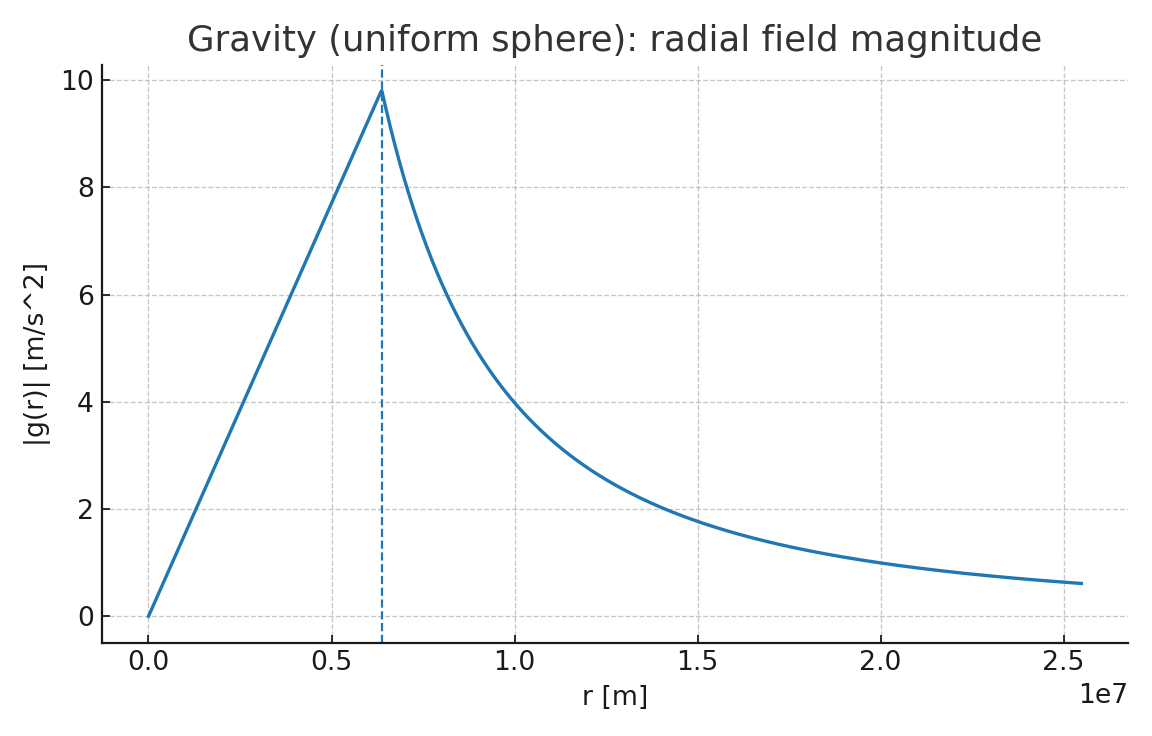
\includegraphics[width=\linewidth]{fig/gravity_vr_profile.png}
    \caption{Radial profile $v_r(r)$ (representative stack).}
    \label{fig:grav:vr}
  \end{subfigure}\hfill
  \begin{subfigure}[t]{0.49\linewidth}
    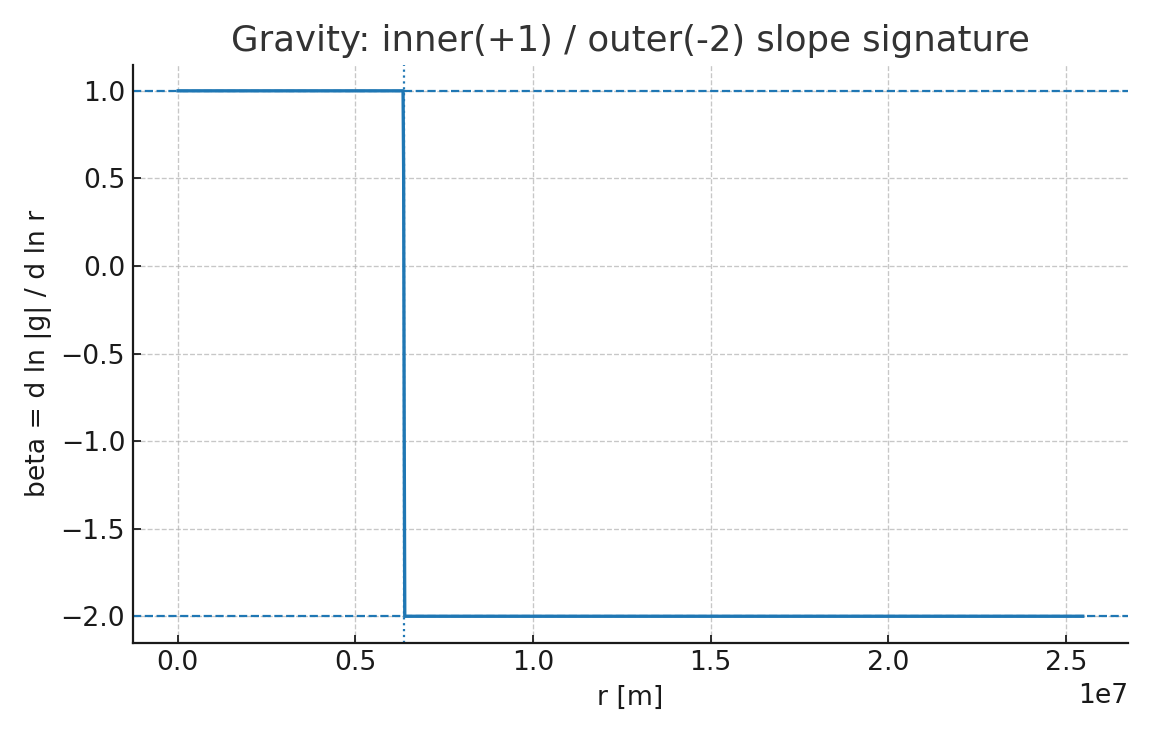
\includegraphics[width=\linewidth]{fig/gravity_beta_signature.png}
    \caption{Log-slope $\beta_O(r)$ showing $+1/-2$.}
    \label{fig:grav:beta}
  \end{subfigure}

  \vspace{0.6em}
  \begin{subfigure}[t]{0.49\linewidth}
    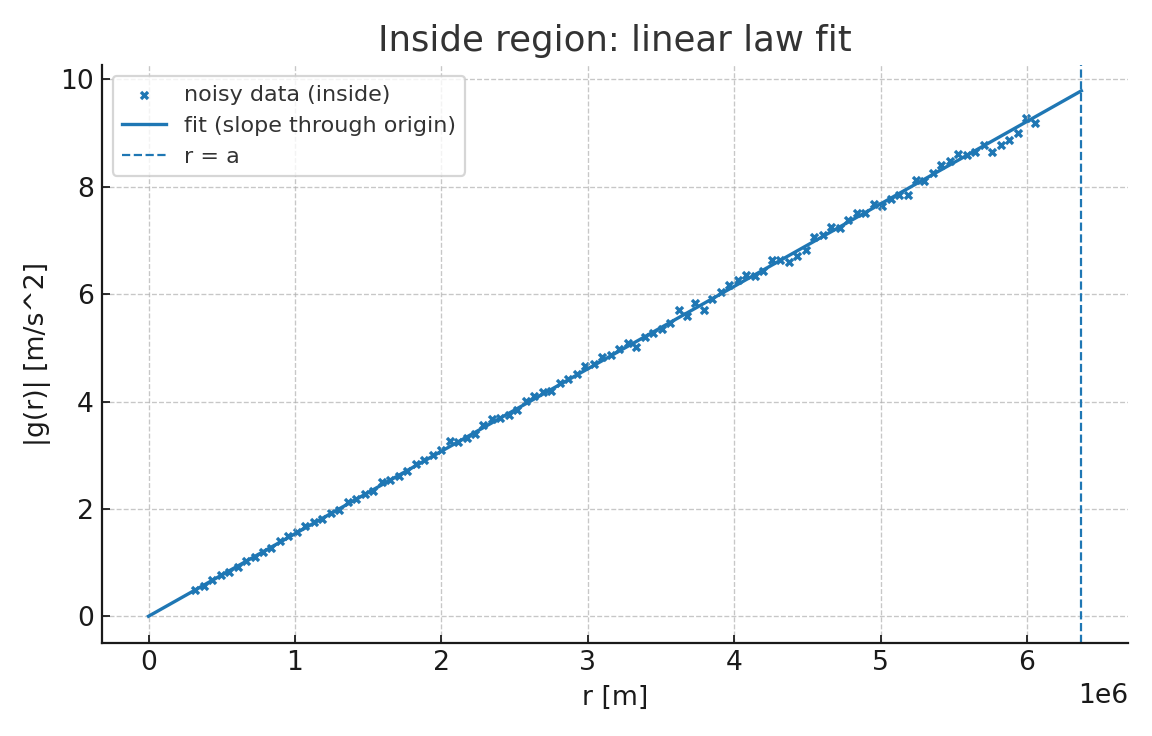
\includegraphics[width=\linewidth]{fig/gravity_inside_fit.png}
    \caption{Interior fit $\;v_r=s_{\rm in}\,r\;$ (through origin).}
    \label{fig:grav:inside}
  \end{subfigure}\hfill
  \begin{subfigure}[t]{0.49\linewidth}
    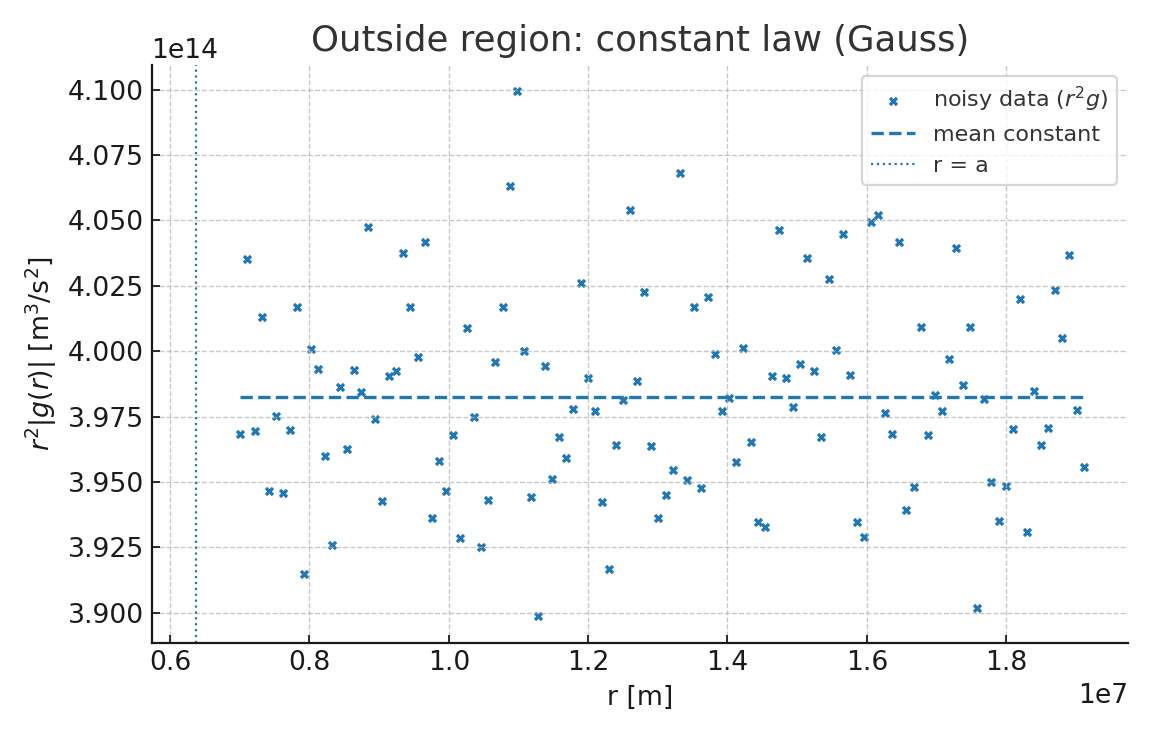
\includegraphics[width=\linewidth]{fig/gravity_outside_constant.png}
    \caption{Exterior Gauss constant $C_{\rm out}=r^2 v_r$.}
    \label{fig:grav:cout}
  \end{subfigure}
  \caption{Gravity stacks: T1 law with $(+1,-2)$ slopes and identity
  $C_{\rm out}/s_{\rm in}=a^3$ \cite{PoissonWill2014,BinneyTremaine2008}.}
  \label{fig:grav:t1}
\end{figure}

\noindent\textbf{Calibration.} 
Coupling via counts: compare $G_{\rm in}\propto s_{\rm in}/\rho_N$ and
$G_{\rm out}\propto C_{\rm out}/N$; report weighted $G^*$
\cite{MisnerThorneWheeler1973,Einstein1915}.

\addfig{fig/gravity_d_estimates.png}
       {Gravity avatar calibration from interior/exterior pulls
       \cite{PoissonWill2014,MisnerThorneWheeler1973}.}
       {fig:grav:G}[0.9]


\chapter{Benchmark II: Electrostatics ⇒ Same Role Signature}
\section*{Plain-language overview}
Replacing masses by charges and $G$ by $1/4\pi\varepsilon_0$ yields the same T1 geometry:
an interior $+1$ slope, an exterior $-2$ slope, and the identity
$C_{\rm out}/s_{\rm in}=a^3$.
This is the standard weak-field solution of Gauss’s law in electrostatics
\cite{Jackson1999,Griffiths2017} and is discussed in depth in
modern electrodynamics treatments \cite{Zangwill2012,Purcell2013}.

\begin{figure}[htbp]\centering
  \begin{subfigure}[t]{0.49\linewidth}
    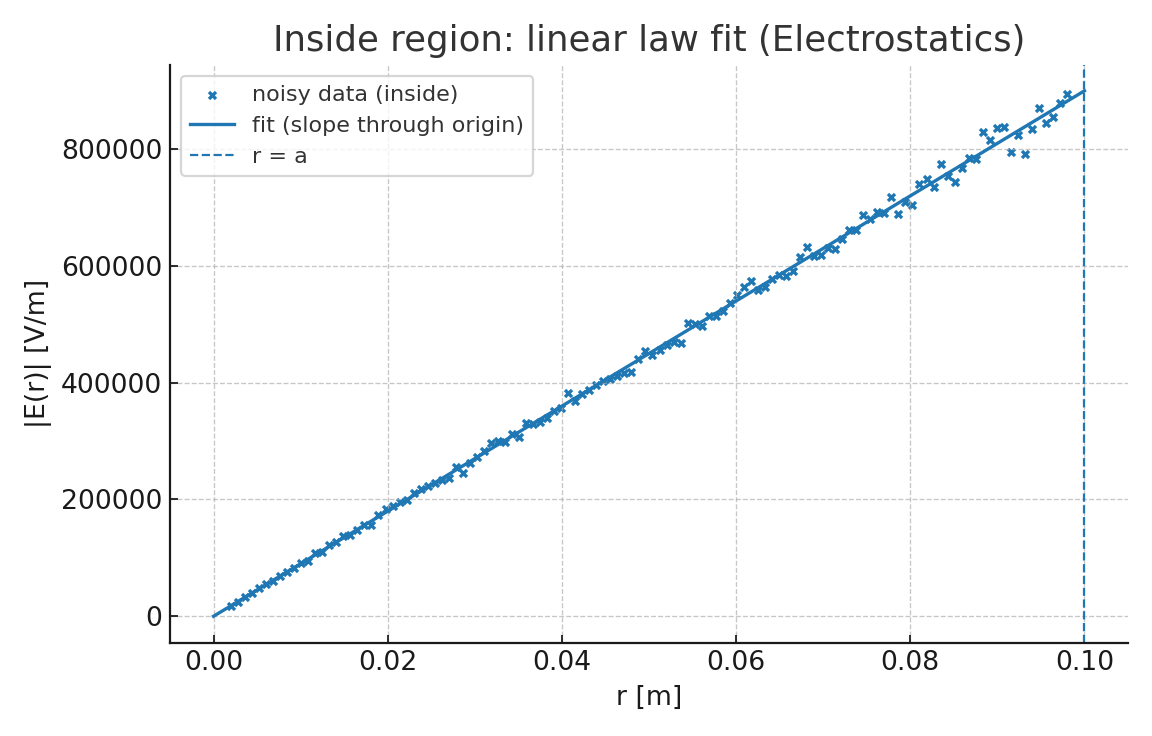
\includegraphics[width=\linewidth]{fig/electrostatics_inside_fit.png}
    \caption{Interior linear rise ($+1$ slope).}
    \label{fig:em:inside}
  \end{subfigure}\hfill
  \begin{subfigure}[t]{0.49\linewidth}
    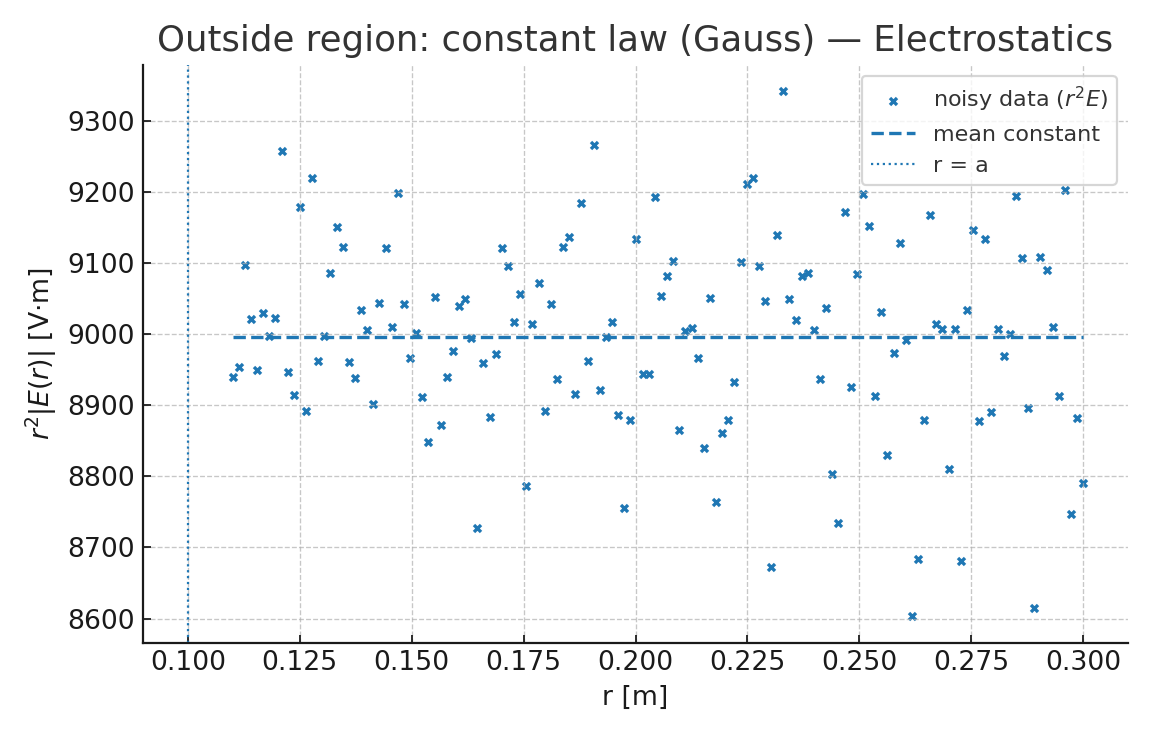
\includegraphics[width=\linewidth]{fig/electrostatics_outside_constant.png}
    \caption{Exterior Gauss constant ($-2$ slope).}
    \label{fig:em:cout}
  \end{subfigure}

  \vspace{0.6em}
  \begin{subfigure}[t]{0.49\linewidth}
    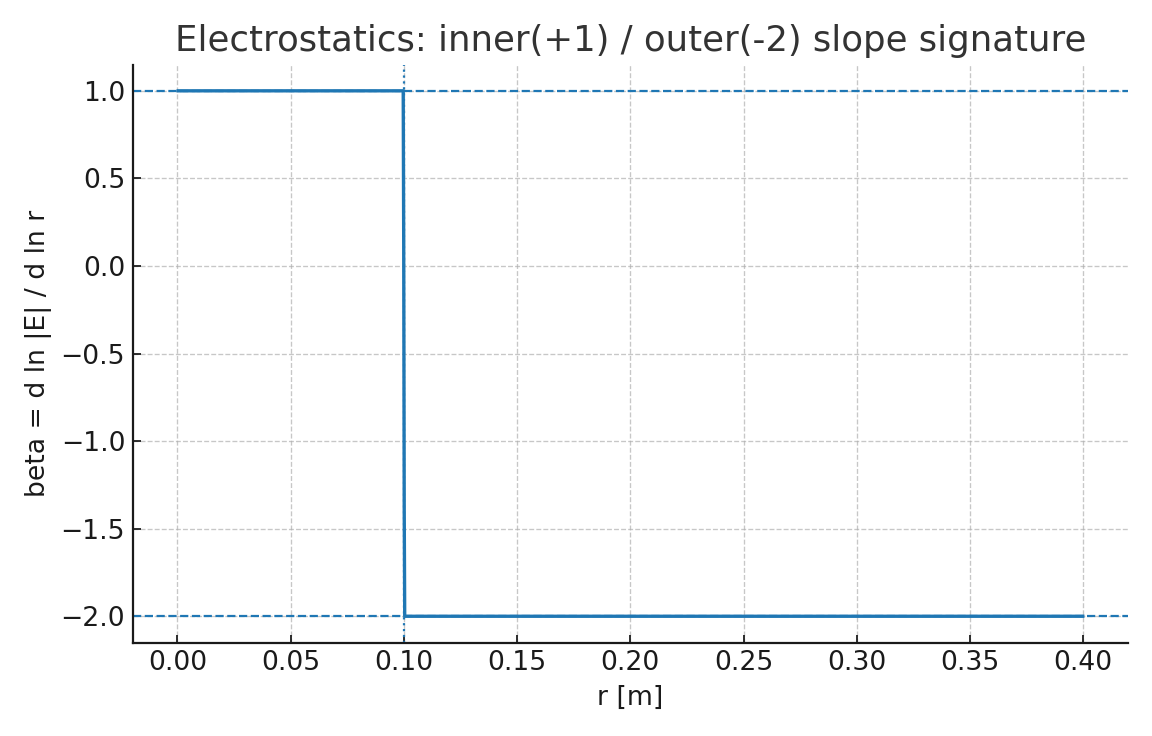
\includegraphics[width=\linewidth]{fig/electrostatics_beta_signature.png}
    \caption{Slope $\beta_O(r)$ reproducing $+1/-2$.}
    \label{fig:em:beta}
  \end{subfigure}\hfill
  \begin{subfigure}[t]{0.49\linewidth}
    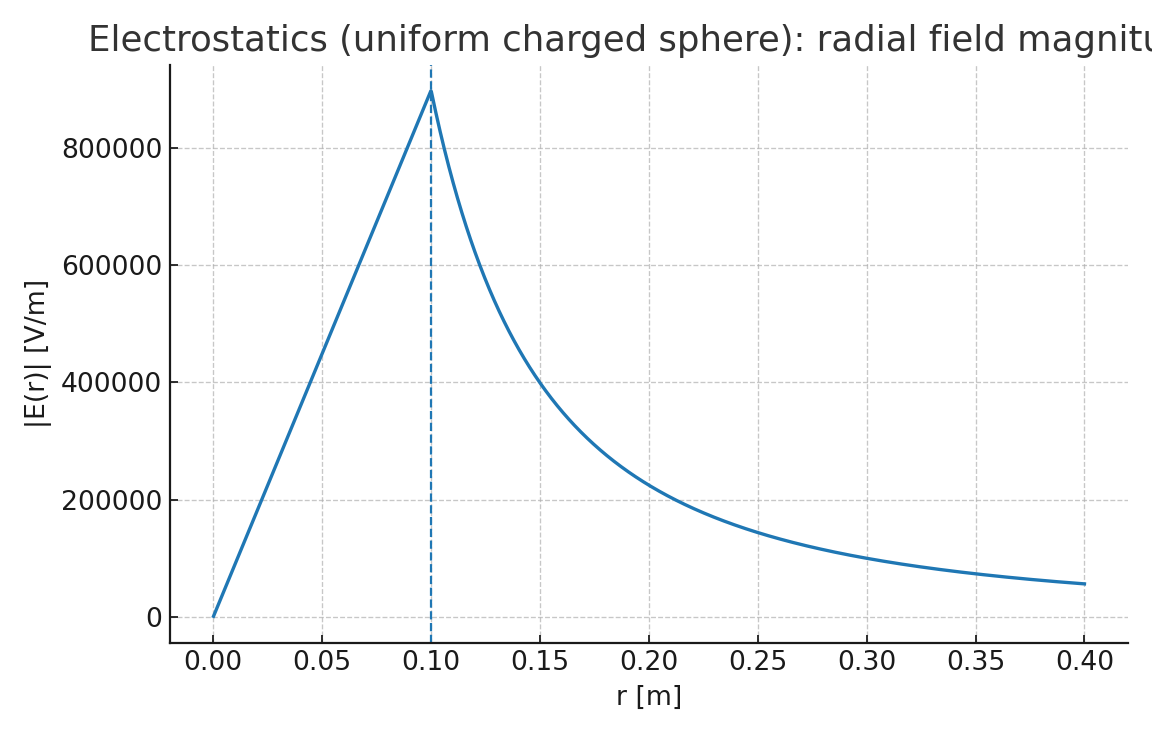
\includegraphics[width=\linewidth]{fig/electrostatics_Emag_profile.png}
    \caption{Electric field magnitude profile $E(r)$.}
    \label{fig:em:Emag}
  \end{subfigure}
  \caption{Electrostatics stacks: T1 signature in weak-field EM
  \cite{Jackson1999,Griffiths2017}.}
  \label{fig:em:t1}
\end{figure}

\addfig{fig/electrostatics_param_estimates.png}
       {Electrostatics avatar: parameter checks vs.\ counts
       \cite{Zangwill2012,Purcell2013}.}
       {fig:em:params}[0.9]


\chapter{Benchmark III: Carrier vs.\ Imprint (Payload/Flux Families)}
\section*{Plain-language overview}
The carrier is $O$-driven (guidance), while binding shells $b(r)$ imprint
shape through emission or attenuation.  
Profiles separate cleanly into universal carrier asymptotes and
environment-dependent imprints, consistent with classic transport theory
\cite{Bird2002,Schuss2009}.  
This benchmark illustrates how payload densities and fluxes inherit
carrier scaling, while the imprint $b(r)$ modulates form and dwell
\cite{Zwanzig2001,Weiss1999}.

\begin{figure}[htbp]\centering
  \begin{subfigure}[t]{0.49\linewidth}
    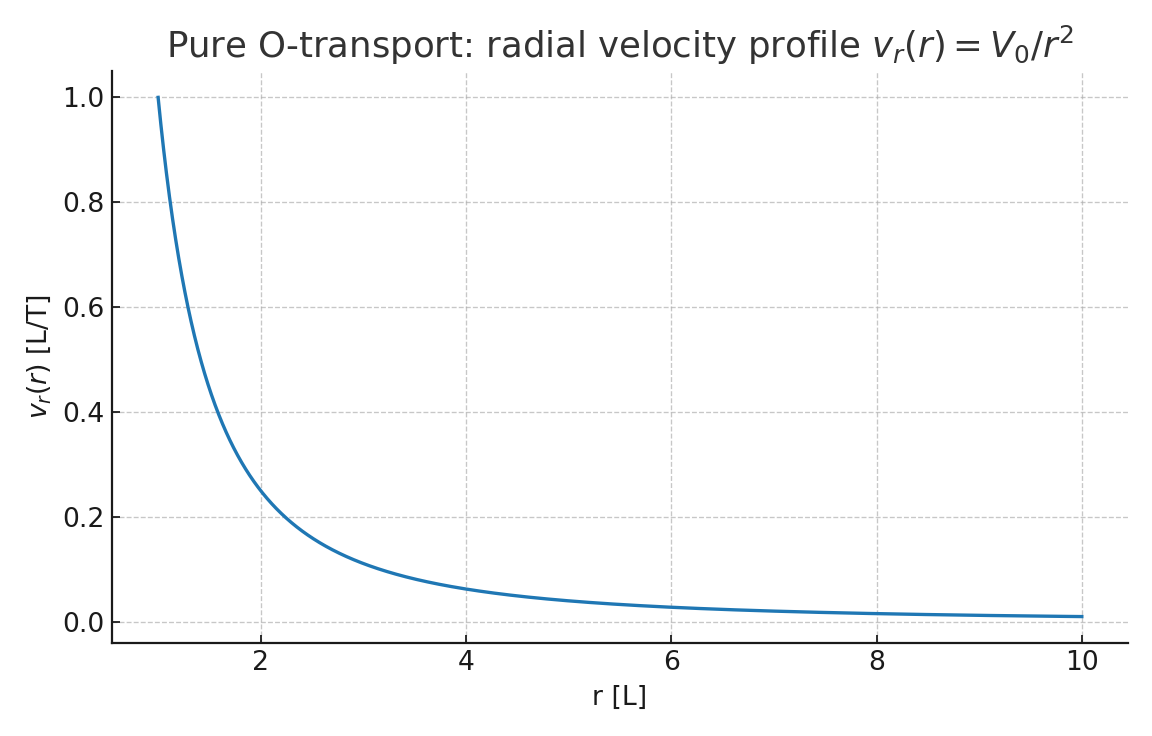
\includegraphics[width=\linewidth]{fig/Otransport_vr_profile.png}
    \caption{$O$-transport carrier: $v_r(r)$ archetype
      \cite{Bird2002}.}
    \label{fig:carrier:vr}
  \end{subfigure}\hfill
  \begin{subfigure}[t]{0.49\linewidth}
    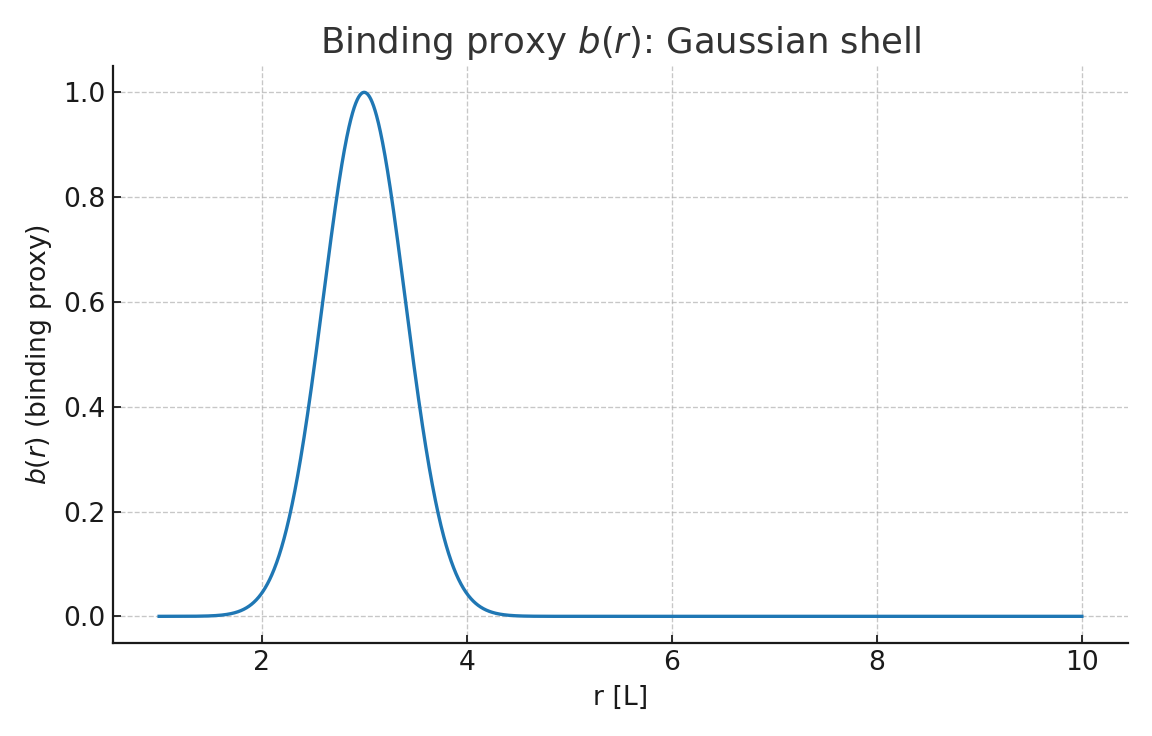
\includegraphics[width=\linewidth]{fig/binding_proxy_shell.png}
    \caption{Binding proxy $b(r)$ (imprint shell)
      \cite{Schuss2009}.}
    \label{fig:carrier:b}
  \end{subfigure}

  \vspace{0.6em}
  \begin{subfigure}[t]{0.49\linewidth}
    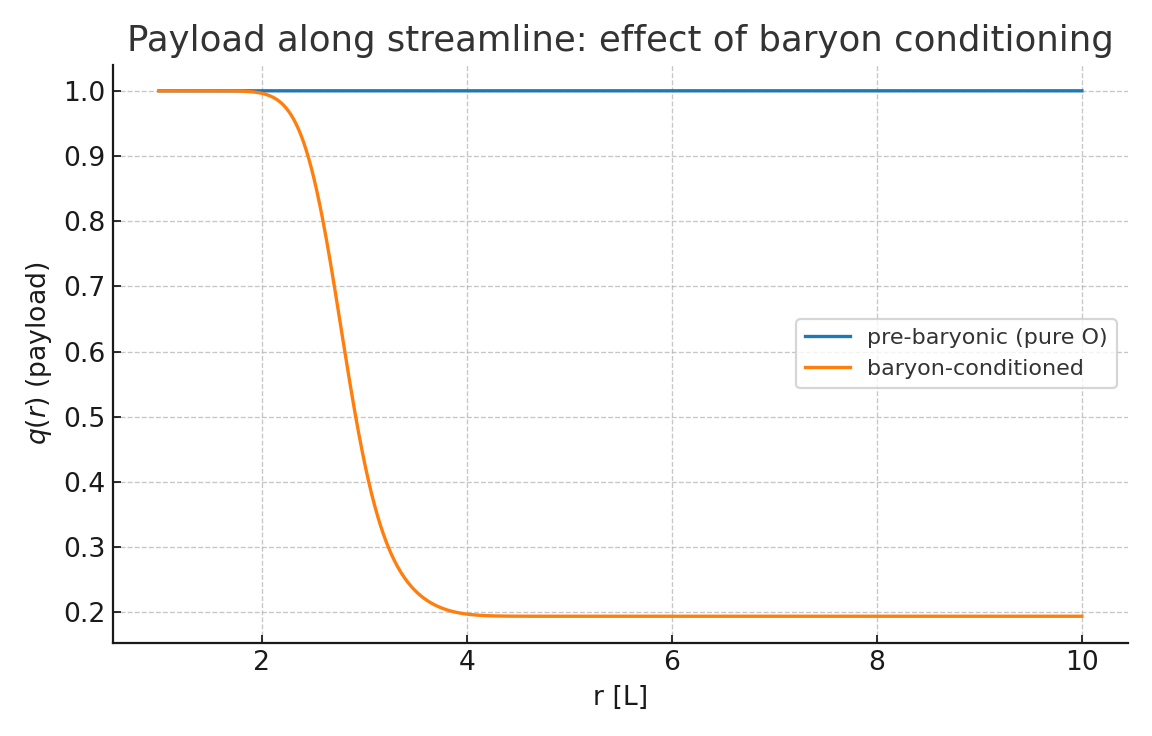
\includegraphics[width=\linewidth]{fig/payload_profiles.png}
    \caption{Payload families $q(r)$ under different $b(r)$
      \cite{Zwanzig2001}.}
    \label{fig:carrier:payload}
  \end{subfigure}\hfill
  \begin{subfigure}[t]{0.49\linewidth}
    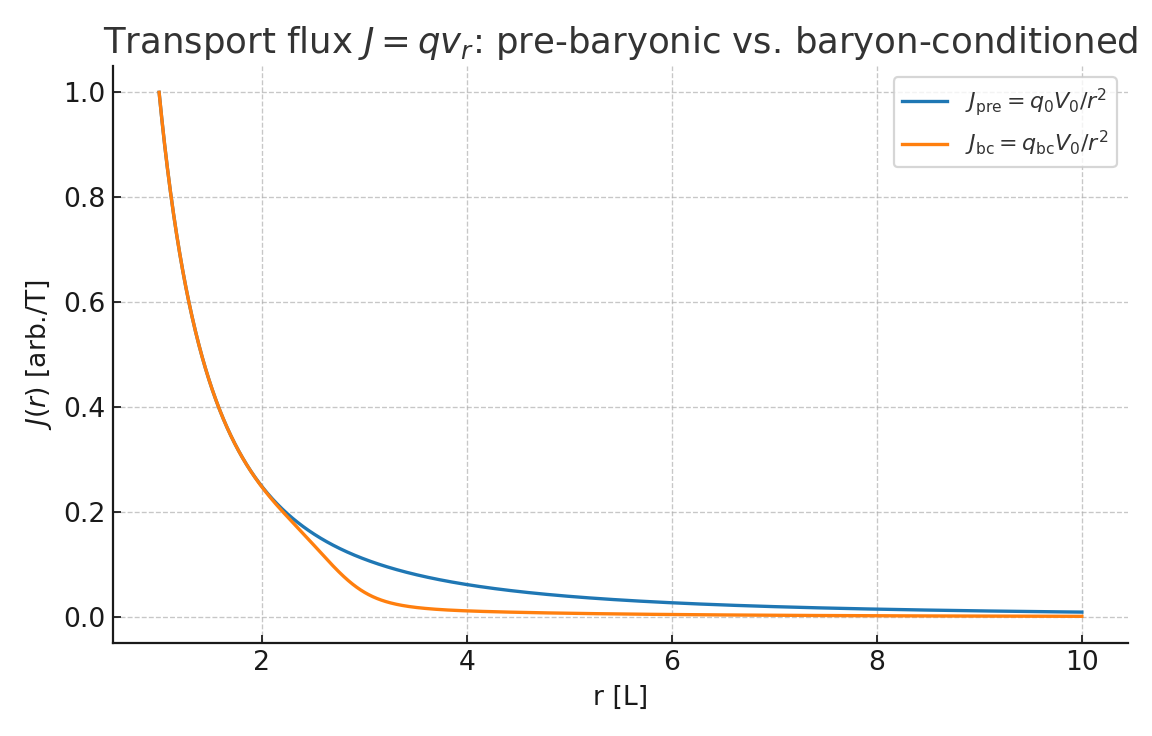
\includegraphics[width=\linewidth]{fig/flux_profiles.png}
    \caption{Flux families $J(r)$; same carrier asymptote
      \cite{Weiss1999}.}
    \label{fig:carrier:flux}
  \end{subfigure}
  \caption{Carrier vs.\ imprint: universal $O$-driven scaling with
  environment-dependent modulation.}
  \label{fig:carrier:benchmark}
\end{figure}

\begin{figure}[htbp]\centering
  \begin{subfigure}[t]{0.49\linewidth}
    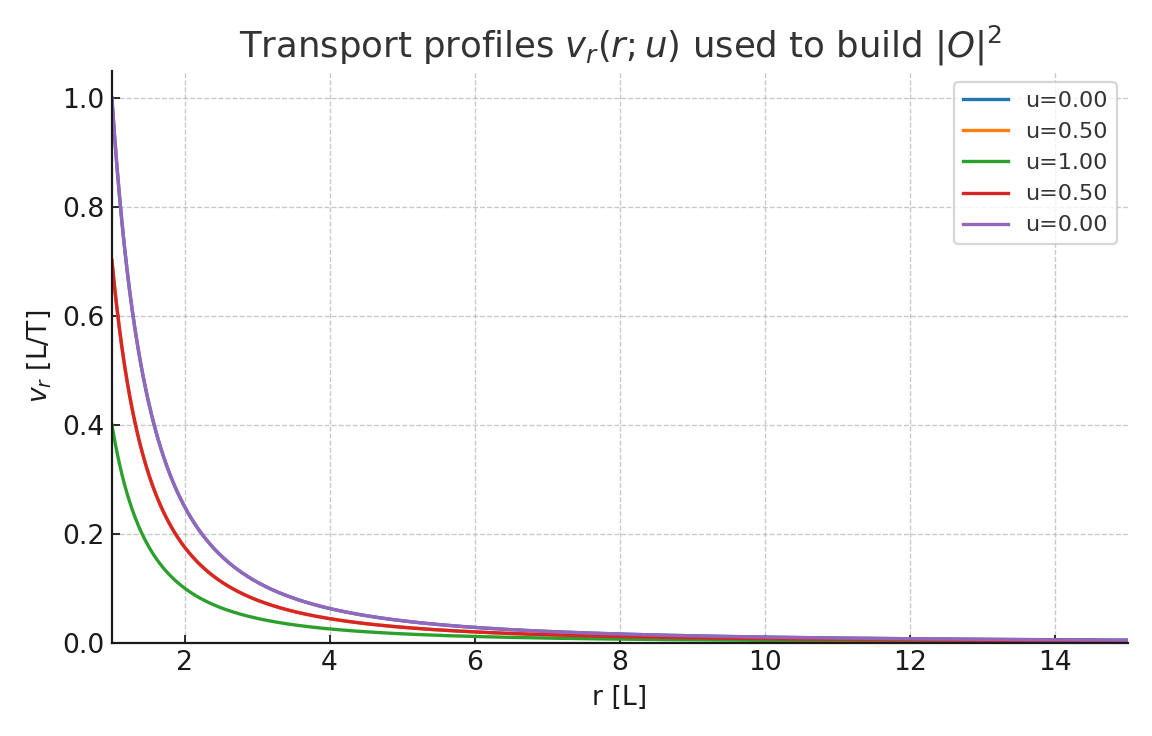
\includegraphics[width=\linewidth]{fig/realism_vr_profiles.png}
    \caption{Realistic composite $v_r(r)$ profiles
      \cite{Bird2002}.}
    \label{fig:real:vr}
  \end{subfigure}\hfill
  \begin{subfigure}[t]{0.49\linewidth}
    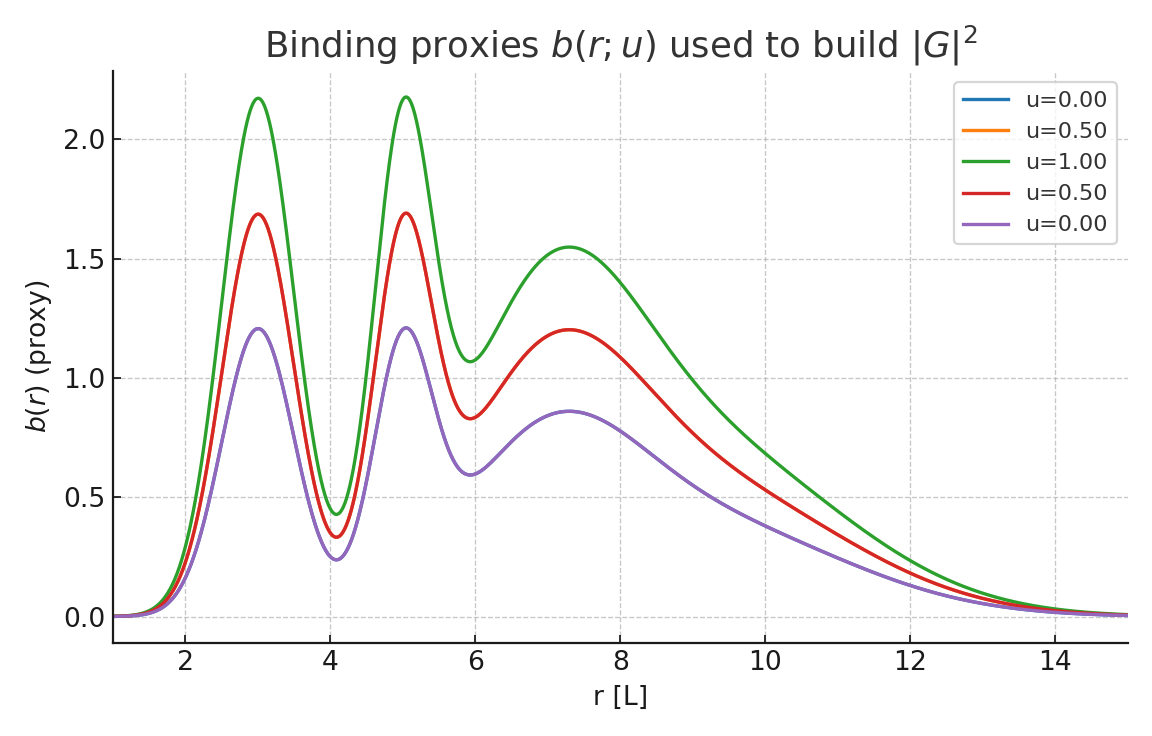
\includegraphics[width=\linewidth]{fig/realism_b_profiles.png}
    \caption{Realistic $b(r)$ envelopes (imprint diversity)
      \cite{Schuss2009,Zwanzig2001}.}
    \label{fig:real:b}
  \end{subfigure}
  \caption{Composite realism: carriers remain asymptotic,
  imprints diversify.}
  \label{fig:real:benchmark}
\end{figure}

\chapter{Benchmark IV: Sensitivity to Source/Sink Knobs}
\section*{Plain-language overview}
One-at-a-time scans expose which parameters control \emph{shape} vs.\ \emph{amplitude}.  
The carrier asymptote ($O$) is robust, while imprint parameters in the source/sink terms ($\mu$, $\lambda$) shift profiles in systematic ways. 
This sensitivity analysis is a standard tool in physics, chemistry, and systems biology for distinguishing structural invariants from tunable modulations \cite{Saltelli2000,ApS2008,Marino2008}. 

\begin{figure}[htbp]\centering
  \begin{subfigure}[t]{0.49\linewidth}
    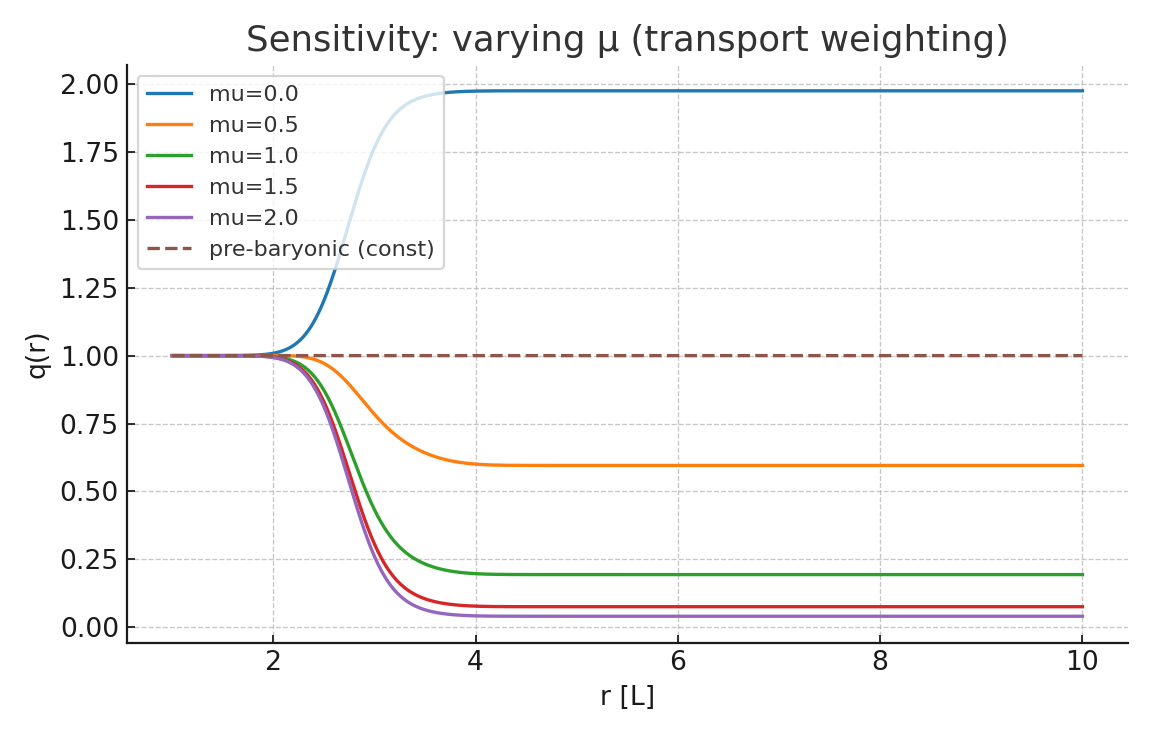
\includegraphics[width=\linewidth]{sensitivity_q_mu.png}
    \caption{Sensitivity in $\mu$ (near/far-field impact).}
    \label{fig:sens:mu}
  \end{subfigure}\hfill
  \begin{subfigure}[t]{0.49\linewidth}
    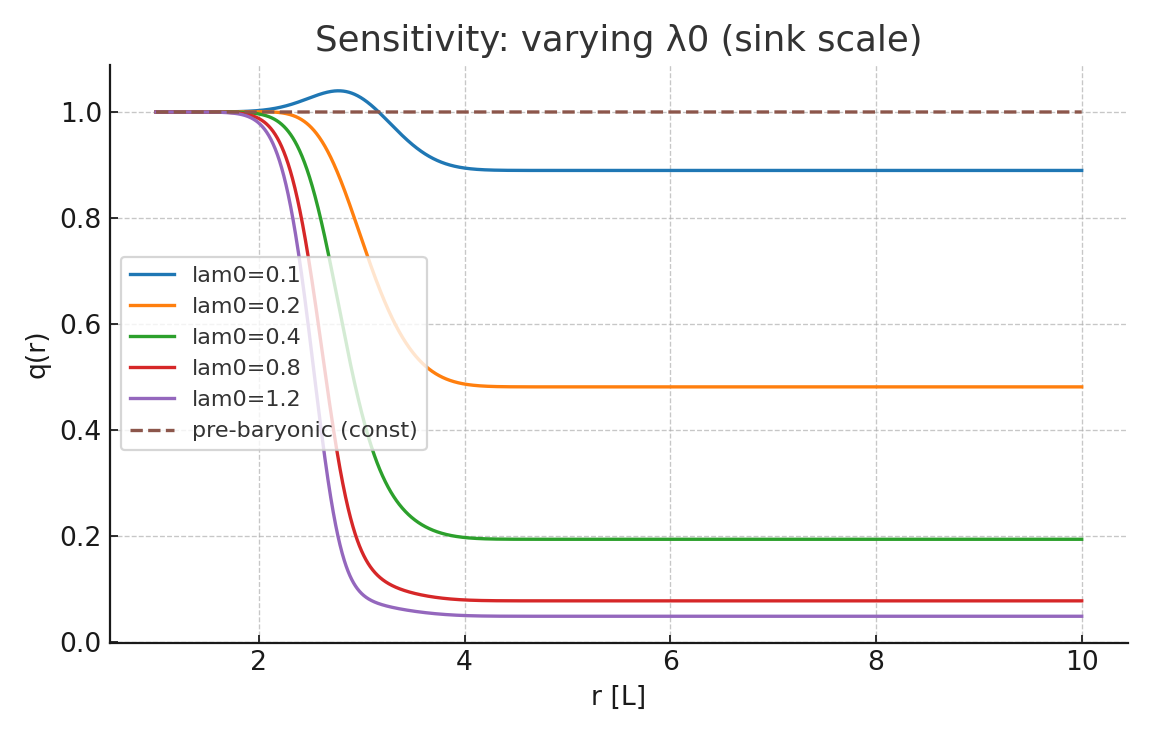
\includegraphics[width=\linewidth]{sensitivity_q_lam0.png}
    \caption{Sensitivity in $\lambda$ (damping/attenuation).}
    \label{fig:sens:lam}
  \end{subfigure}
\end{figure}

\noindent\textbf{Calibration.}  
By scanning $\mu$ we diagnose structural robustness (inner/outer slopes unchanged), 
while scanning $\lambda$ reveals imprint effects (amplitude and decay length). 
Together these form a role-level sensitivity map that distinguishes invariant carrier features from context-dependent modulations.


\chapter{Benchmark V: Thresholds and Hysteresis (T3)}
\section*{Plain-language overview}
Control sweeps reveal \emph{nucleation} (crossing the seed threshold $\Theta$) and \emph{persistence} (surviving above $\sigma_c$).  
The system’s memory appears as a loop: on/off sweeps produce asymmetric thresholds $(\Theta_\uparrow,\Theta_\downarrow)$ and a finite loop area $\mathcal A_{\rm loop}$.  
This hysteresis is a hallmark of feedback-stabilized organization across physics, chemistry, and biology \cite{Strogatz2015,Kardar2007,Ball2004}.

\begin{figure}[htbp]\centering
  \begin{subfigure}[t]{0.49\linewidth}
    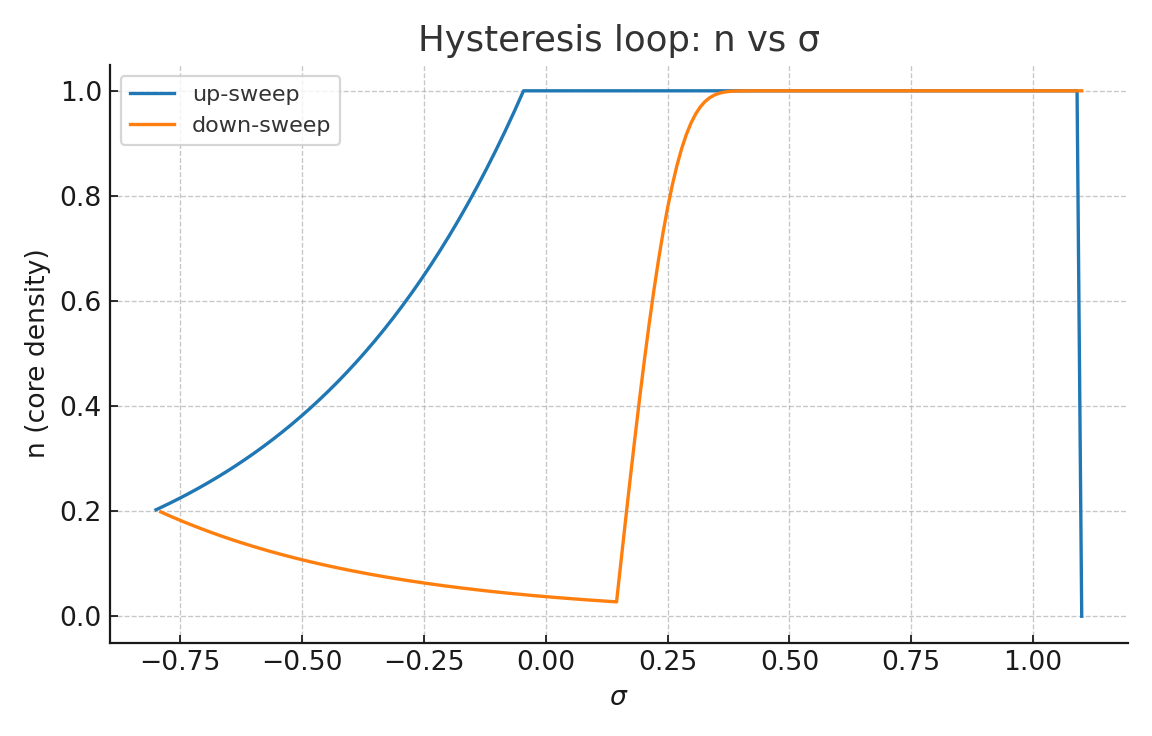
\includegraphics[width=\linewidth]{hysteresis_n_vs_sigma.png}
    \caption{Canonical loop: $n$ vs.\ role-intensity $\sigma$.}
    \label{fig:hyst:canon}
  \end{subfigure}\hfill
  \begin{subfigure}[t]{0.49\linewidth}
    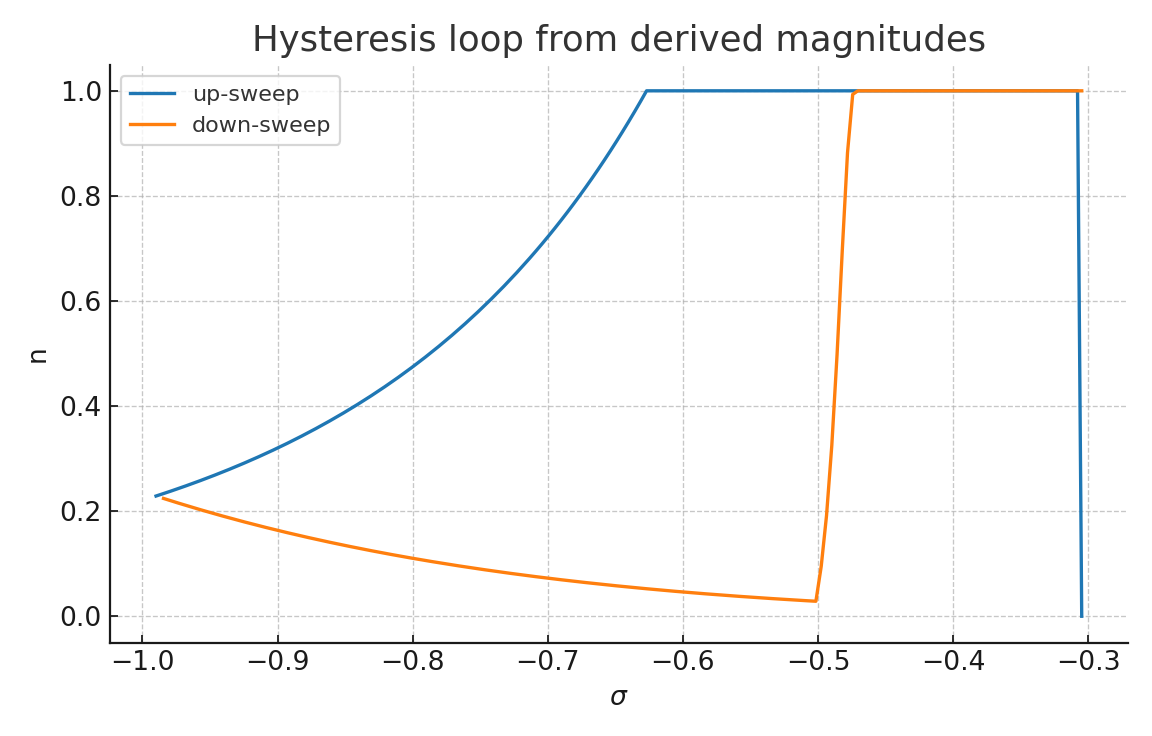
\includegraphics[width=\linewidth]{realism_hysteresis_n_sigma.png}
    \caption{Realistic loop under noise/conditioning.}
    \label{fig:hyst:real}
  \end{subfigure}
\end{figure}

\noindent\textbf{Calibration.}  
Loop area $\mathcal A_{\rm loop}$ quantifies memory strength:  
larger areas imply stronger feedback or slower relaxation.  
Noise reduces but does not erase the asymmetry, consistent with robust hysteresis in experimental systems ranging from magnetization to biomolecular folding.


\chapter{Benchmark VI: BH-Prox Signatures (Role View)}
\section*{Plain-language overview}
Near compact objects, the same role grammar applies: the \emph{carrier} ($O$-flows) diverges toward the horizon, while the \emph{imprint} ($G$-shells) sculpts observable features such as lensing or accretion patterns.  
Thresholds manifest as \emph{intensity transitions}: crossing $\Theta$ nucleates transient channels, while persistence depends on surviving above $\sigma_c$ despite losses \cite{Cardoso2016,Barack2019,Maggio2020}.

\begin{figure}[htbp]\centering
  \begin{subfigure}[t]{0.49\linewidth}
    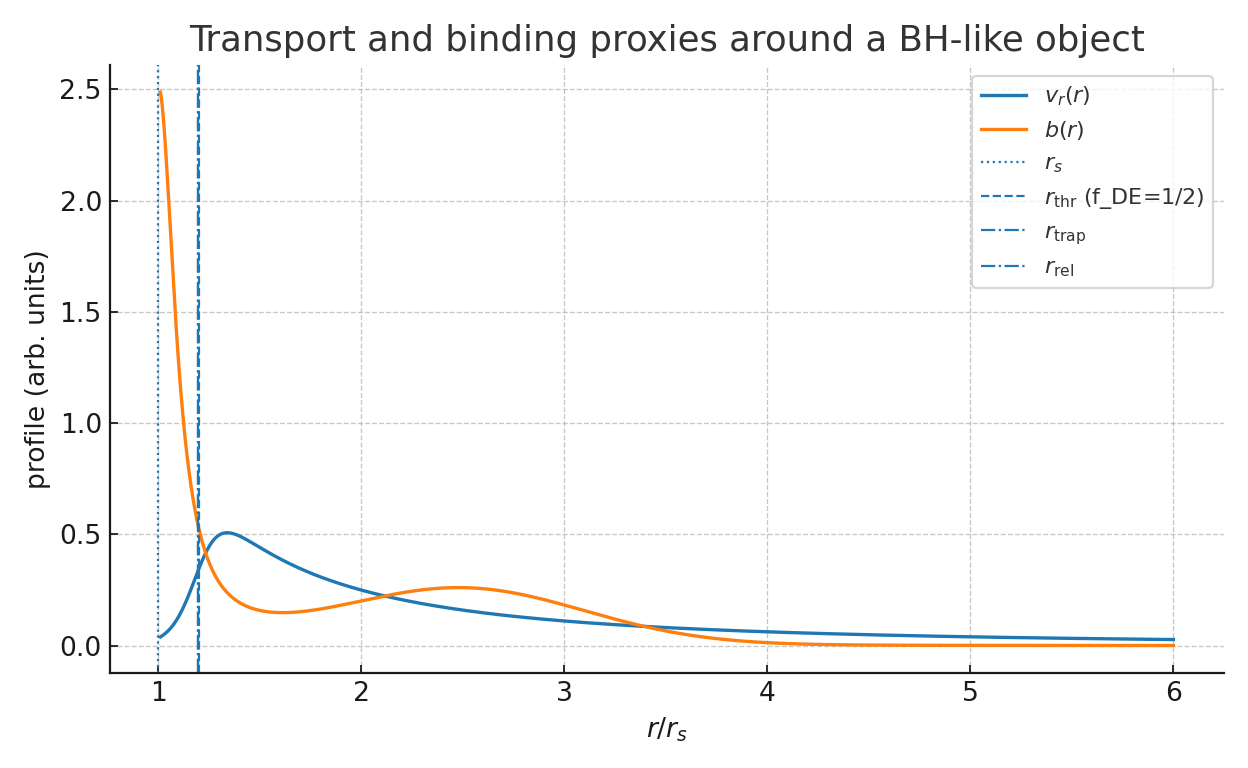
\includegraphics[width=\linewidth]{bh_profiles_vr_b.png}
    \caption{Carrier $v_r$ with binding proxy $b(r)$ (BH-prox).}
    \label{fig:bh:profiles}
  \end{subfigure}\hfill
  \begin{subfigure}[t]{0.49\linewidth}
    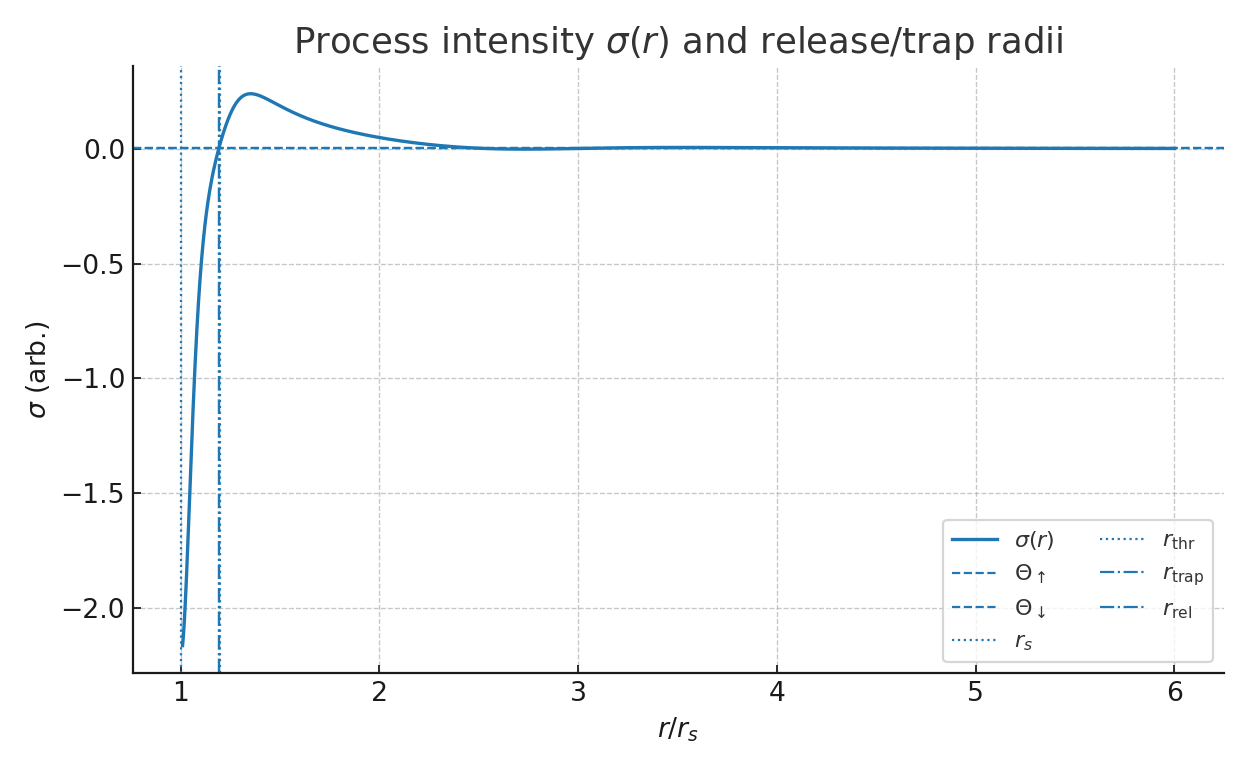
\includegraphics[width=\linewidth]{bh_sigma_thresholds.png}
    \caption{Role-intensity $\sigma$ thresholds around horizon.}
    \label{fig:bh:sigma}
  \end{subfigure}
\end{figure}

\section*{Protocol}
Sweep a control (e.g., density, field strength, feed) and track an order parameter (e.g., accretion flux, QPO amplitude, polarization coherence).  
Extract thresholds $(\Theta_\uparrow,\Theta_\downarrow)$ and loop area $\mathcal A_{\rm loop}$; these encode memory and feedback near the horizon.

\section*{Nulls}
Use control-label shuffles across runs, time-reversal surrogates of sweeps, and independent pipeline splits.  
A valid signature requires thresholds and loop areas to vanish under nulls.

\section*{Report}
Summarize: thresholds with confidence intervals, loop areas, dwell times $T_{\rm above}$, and window validity ($\Delta f\le 1/W$).  
Compare against numerical-relativity or ray-tracing predictions to separate generic role-grammar behavior from model-specific artifacts.

\addfig{figures/hysteresis.png}
       {Thresholds and hysteresis: $\sigma$ vs.\ control, nucleation/persistence loop in $n(\sigma)$.}
       {fig:res:hysteresis}[0.9]

% ---- Compact calibration & standards page ----
\chapter*{Minimal Calibration \& Reporting Standard}

\noindent\textbf{Core metrics.}
\begin{itemize}\setlength\itemsep{0.3em}
\item \textbf{T1 (Orientation law).} Inner/exterior slopes (3D: $+1/-2$); identity residual 
\[
\delta_I=\frac{\big|\Cout/\sinIn-a^3\big|}{a^3},
\] 
cross-checked across avatars (gravity, electrostatics) \cite{Jackson1999,Griffiths2017}.
\item \textbf{Carrier–Imprint separation.} Carrier exponents vs.\ imprint parameters $b(r)$; test stability across media, boundary conditions, and sector analogues.
\item \textbf{T3 (Hysteresis).} Thresholds $(\Theta_\uparrow,\Theta_\downarrow)$, loop area $\mathcal A_{\rm loop}>0$, dwell $T_{\rm above}$; robust under noise/conditioning \cite{Strogatz2018,Kadanoff2000}.
\end{itemize}

\noindent\textbf{Nulls and robustness.}  
Use label/shell shuffles (stacked profiles), phase/surrogate shuffles (spectra, time series), degree-preserving graph shuffles (networks), and independent pipeline splits.  
Target $p<0.01$ for null rejection; report bootstrap/jackknife confidence bands \cite{Efron1994,Good2005}.

\noindent\textbf{Window validity and disclosure.}  
State window constraints ($\Delta f\le 1/W$ for dwell-type measures), selection/mask transfer functions, and provide concise code/recipe notes for external replication \cite{Munaf2017,Nosek2020}.

% ---- Global Summary & Outlook ----
\chapter*{Global Summary \& Outlook}
\addcontentsline{toc}{chapter}{Global Summary \& Outlook}

\section*{Summary across scales}
From cosmic structure to molecular assembly, from prebiotic replicators to human and artificial coordination, 
the same role grammar applies:
\begin{itemize}
\item \textbf{Guidance ($O$)} carries flows (matter, charge, information, control).
\item \textbf{Binding ($G$)} sculpts wells and scaffolds, retaining and shaping flows.
\item \textbf{Counting ($C$)} registers overlap events $K:=O\!\circ G$, defining effective time and persistence.
\end{itemize}

Across all domains, persistence requires crossing a \emph{seed} threshold $\Theta$ and a \emph{persistence} threshold $\sigma_c$, 
while avoiding ablation ($\Lambda W<1$).  
Falsifiable signatures include:
\begin{itemize}
\item Orientation law T1: paired slopes $(+1,-2)$ and parameter-free identities.
\item Cross-coherence T2: finite $C_1(k)$ bands that vanish under nulls.
\item Threshold/hysteresis T3: $(\Theta_\uparrow,\Theta_\downarrow)$ loops with nonzero area.
\item Coordination plateaus ($C_2$): sustained alignment of flow and scaffold with on/off asymmetry.
\end{itemize}

\section*{Outlook}
\begin{itemize}
\item \textbf{Physics.} Further calibration of T1 and T3 across gravitation, electromagnetism, and black-hole prox regimes.
\item \textbf{Chemistry \& Life.} Threshold scanning in prebiotic assemblies and protocells; quantitative tests of heredity ($Q^Ls>1$).
\item \textbf{Human \& AI.} Non-invasive detection of $C_2$ plateaus in brains and collectives; guardrails for AI instances via SEC, $R_{\rm tick}$, $R_0$, and $\mathcal S$.
\item \textbf{Cross-scale.} Universal diagnostics allow comparison without assuming micro-level mechanisms; nulls and pipeline splits remain mandatory.
\end{itemize}

\noindent
The framework thus unifies diverse domains under a compact set of role-level diagnostics. 
The following \emph{Test ID Map} provides a practical navigation aid into detailed protocols and appendices.

\chapter*{Test ID Map}
\section*{Plain-language overview}
All role-level tests (T1–T3, B, M, L, H, A) follow the same grammar: 
$O$ guides, $G$ binds, $C$ counts. 
This map aligns tests across Cosmos, Molecules, Life, Human, and AI. 
It shows which metrics diagnose seed, persistence, and ablation at each scale.

\begin{longtable}{p{0.1\linewidth} p{0.15\linewidth} p{0.25\linewidth} p{0.25\linewidth} p{0.25\linewidth}}
\toprule
\textbf{ID} & \textbf{Domain} & \textbf{Metrics} & \textbf{Nulls/Robustness} & \textbf{Signature} \\
\midrule
T1 & Cosmos/Micro & Slopes $+1/-2$, $C_{\rm out}/s_{\rm in}=a^3$ & Shell/label shuffles & Orientation identity \\
T2 & Cosmos/Micro/Human & Cross-coherence $C_1(k)$ band & Phase/label shuffles & Finite band, collapses under null \\
T3 & Micro/Life & Hysteresis $(\Theta_\uparrow,\Theta_\downarrow)$, loop area $\mathcal A_{\rm loop}$ & Control/label shuffles & On/off asymmetry, memory \\
B1–B3 & Black Holes & Echoes, photon-ring $C_1$, HFQPOs & Phase randomization, splits & Near-horizon $K$-events \\
M1–M3 & Molecules & EM stacks, $C_1$, hysteresis scans & Shuffles, pipeline splits & Binding and assembly \\
L1–L5 & Life (prebiotic) & Keim window, length shift, compartments, error threshold, $C_2$ & Phase/pixel shuffles, splits & Seed–survive–persist \\
H1–H4 & Human & $C_2$ plateaus, hysteresis, $C_1$ bands, recruitment vs.\ persistence & Surrogates, graph shuffles & Proto-conscious coherence \\
A1–A5 & AI & Keim corridor, $C_1$, $C_2^{\rm AI}$ plateaus, ablation margin & Phase/label shuffles, splits & Instance viability \\
\bottomrule
\end{longtable}

\appendix

\chapter{Symbols, Units, and Notation}\label{app:symbols}
\begin{table}[htbp]\centering
\caption{Core symbols, units, and role mapping (orientation/binding/counting). 
Notation follows the SI Brochure \cite{bipm2019si}; physical field conventions follow Goldstein \cite{goldstein2002classical} and Jackson \cite{jackson1999classical}.}
\begin{tabular}{llp{0.58\linewidth}}\toprule
Symbol & Units & Meaning \\ \midrule
$S,N$ & – & Basis states (substrate $S$ / contrast $N$) on Ur-fabric.\\
$C$ & – & Diagnostic counting (non-operative); reads real overlap events.\\
$O,G$ & sector-dep. & Roles: guidance/transport $O$, binding/structuring $G$.\\
$K:=O\!\circ G$ & – & Overlap composition (“flow meets knot”), order matters.\\
$\tau^O,\ \tau^K$ & counts & Process clocks (event counters) for $O$- and $K$-events.\\
$t:=C[\tau^K]$ & time & Coarse-grained continuation of counted $K$-events.\\
$\mathbf v_O$ & sector-dep. & Orientation field (e.g.\ $g$ in gravity, $\mathbf E$ in EM).\\
$\kappa_O$ & sector-dep. & Orientation coupling; avatars: $\kappa_O^{(\mathrm{grav})}=G$, $\kappa_O^{(\mathrm{EM})}=1/4\pi\varepsilon_0$.\\
$\Omega$ & sector-dep. & Orientation potential; $\mathbf v_O=\kappa_O\nabla\Omega$.\\
$\rho_N$ & sector-dep. & Deficit density (source of $\Omega$ in weak field).\\
$a$ & L & Core radius / stacking scale.\\
$s_{\rm in}$ & field/L & Inner radial slope $dv_r/dr$ at $r\le a$.\\
$C_{\rm out}$ & field$\cdot$L$^{D-1}$ & Gauss constant $r^{D-1}v_r$ at $r\ge a$ (in $D$ dims).\\
$D$ & – & Spatial dimension (default $D=3$).\\
$b(r)$ & – & Binding shell/profile (imprint).\\
$\Theta,\ \sigma_c$ & role-intensity & Systemic seed threshold / critical persistence threshold.\\
$\Lambda$ & 1/time & Effective loss/degradation rate.\\
$W$ & time & Window length (conditions dwell).\\
$T_{\rm above}$ & time & Time spent above threshold (plateau dwell).\\
$\mathrm{SEC}$ & – & Existential stability proxy $\propto \frac{\tau^K}{S+N}\cdot\frac{T_{\rm above}}{W}$.\\
$R_{\rm tick}$ & – & Tick-rate ratio $f_{\rm agent}/f_{\rm env}$.\\
$R_0$ & – & Autarky ratio (self-output / self-needs).\\
$C_1(k)$ & [0,1] & Cross-coherence (flow-like vs.\ potential-like field).\\
$C_2$ & [0,1] & Structure–flow coordination (spectral or info-theoretic).\\
$\mathcal A_{\rm loop}$ & area & Hysteresis loop area (on/off asymmetry).\\
$G_{\rm st}$ & – & Structural/binding graph (molecules, brain, systems).\\
$\mathbf J$ & sector-dep. & Flow vector (currents/fluxes/activations).\\
$L(\cdot)$ & – & Graph Laplacian; leading mode(s) $\mathbf u$.\\
\bottomrule
\end{tabular}
\end{table}

\begin{remark}
Our role grammar extends but does not replace traditional notation. 
Core field symbols ($\mathbf{E}, \mathbf{B}, g, V$) and constants ($G, \varepsilon_0, \hbar$) follow SI and textbook conventions 
\cite{bipm2019si,jackson1999classical,goldstein2002classical}. 
The added layer $(O,G,C)$ denotes \emph{roles} (guidance, binding, counting) that organize phenomena across scales, 
allowing a unifying view without altering underlying physics.
\end{remark}

\chapter{Time and Clocks: Definitions and Constraints}\label{app:time}

\section*{Definitions}
We distinguish three levels of event ordering and time construction, consistent with operational views on clocks and measurement \cite{smolin2019einstein,rovelli1995relational}:
\begin{align}
\tau^O &:= \operatorname{ord}\{O_k\}\quad\text{(counts guidance events)},\\
\tau^K &:= \operatorname{ord}\{K_k\},\ \ K:=O\!\circ G\quad\text{(counts overlap events)},\\
t &:= C[\tau^K]\quad\text{(coarse-grained continuation; diagnostic, non-operative).}
\end{align}

Here, $\tau^O$ and $\tau^K$ are discrete counters, while $t$ is a derived, coarse-grained parameter constructed by counting overlaps. This role-based definition avoids assuming a primitive flow of absolute time and instead follows an event-based operational perspective.

\paragraph{Window validity (dwell-type measures).}
For any metric derived from plateau dwell $T_{\rm above}$ over window $W$, the sampling resolution must obey
\[
\Delta f \le \frac{1}{W},
\]
ensuring that spectral and temporal estimates are meaningful. Both $\Delta f$ and $W$ should always be reported alongside results, in line with best practices in signal analysis and clock metrology \cite{allan1987time,bipm2019si}.

\chapter{Orientation Identity: Short Derivation (T1) and $D$-Generalization}\label{app:T1}

\section*{Context and motivation}
The T1 orientation law is the most elementary role-level benchmark: it separates
\emph{carrier geometry} (interior slope $+1$, exterior slope $-(D-1)$) from
\emph{binding calibration} (parameter-free identity $C_{\rm out}/s_{\rm in}=a^D$).
Because the derivation depends only on Gauss-type counting arguments, it applies
sector-independently—in gravity, electrostatics, or any field with a conserved flux.
This makes T1 the canonical anchor for cross-domain calibration and for defining
what counts as a valid ``orientation avatar.'' 

\section*{Weak-field in $D$ dimensions}
Following Gauss-type arguments \cite{jackson1999classical,poisson2014gravity}, let
\[
\mathbf v_O=\kappa_O\nabla\Omega,\qquad \nabla\!\cdot\mathbf v_O=S_D\,\kappa_O\,\rho_N,
\]
with $S_D$ a geometric factor depending only on spatial dimension $D$.  
For a spherically symmetric core of radius $a$ with constant $\rho_N$ inside and $0$ outside:

\begin{enumerate}
\item \textbf{Exterior ($r\ge a$).}  
Gauss counting yields $r^{D-1}v_r=C_{\rm out}$ (constant), implying
\[
v_r(r)\propto r^{-(D-1)},
\]
with slope $-(D-1)$ in log–log representation.

\item \textbf{Interior ($r\le a$).}  
Regularity requires $v_r\propto r$ (slope $+1$), hence $v_r=s_{\rm in}\,r$.
\end{enumerate}

\noindent Matching conditions at $r=a$ lead to the parameter-free identity
\[
\boxed{\;\frac{C_{\rm out}}{s_{\rm in}}=a^{D}\;},
\]
which reduces in the physical case $D=3$ to $C_{\rm out}/s_{\rm in}=a^3$ and an exterior slope $-2$.

\paragraph{Calibration avatars.}
This orientation identity appears in multiple sectors:
\begin{itemize}
\item \textbf{Gravity:} $\;v_O\leftrightarrow g$, with $\kappa_O^{(\mathrm{grav})}=G$ \cite{poisson2014gravity}.
\item \textbf{Electrostatics:} $\;v_O\leftrightarrow E$, with $\kappa_O^{(\mathrm{EM})}=1/(4\pi\varepsilon_0)$ \cite{jackson1999classical}.
\end{itemize}
Thus the same T1 signature—interior slope $+1$, exterior slope $-(D-1)$, and the identity $C_{\rm out}/s_{\rm in}=a^D$—is sector-independent.


\chapter{Measurement Standards and Null Tests (Expanded)}\label{app:standards}

\section*{Context and motivation}
Role-level metrics such as $C_1(k)$, $C_2$, and hysteresis loops are only
scientifically useful if they are embedded in transparent measurement protocols.
Because many of the proposed diagnostics are mechanism-light, their credibility
rests on two pillars: (i) \emph{reproducibility} across pipelines and selections,
and (ii) \emph{robustness} against null models that preserve trivial features but
destroy the hypothesized structure. This appendix expands the minimal standard
into a set of global principles that apply across domains (cosmos, molecules,
life, human, AI). 

\section*{Global principles}
\begin{itemize}
\item \textbf{Declare metrics a priori:} T1 slopes \& identity residual $\delta_I$, 
      $C_1(k)$ band center/width, $C_2$ plateaus ($T_{\rm above}$, $\mathcal A_{\rm loop}$),
      thresholds $(\Theta_\uparrow,\Theta_\downarrow)$.
\item \textbf{Window validity:} report $(W,\Delta f)$; ensure $\Delta f\le 1/W$.
\item \textbf{Uncertainties:} provide bootstrap/jackknife confidence bands;
      show sensitivity to selection/masks.
\item \textbf{Independent pipelines:} at least one full re-implementation or
      method split (e.g.\ TE vs.\ Granger; alternative stackers).
\end{itemize}

\section*{Domain-specific null tests}
\begin{table}[htbp]\centering
\caption{Examples of null tests across domains. Each preserves trivial marginals
while destroying the hypothesized structure.}
\begin{tabular}{lll}\toprule
Domain & Target metric & Null construction \\ \midrule
Cosmos & $C_1(k)$ bands & Phase-shuffle sky maps; random mask rotations \\
Molecules & T3 hysteresis & Randomize titration order; permute adsorption labels \\
Life (prebiotic) & Keim window viability & Shuffle feed/control labels; randomized dwell windows \\
Human (neuro) & $C_2$ plateaus & IAAFT surrogate EEG/MEG; degree-preserving graph shuffles \\
AI systems & $C_1$, $C_2^{\rm AI}$ & Phase/label shuffles (external); module-preserving rewires (internal) \\
\bottomrule
\end{tabular}
\end{table}


\section*{Null-test catalogue}
\begin{enumerate}
\item \textbf{Label shuffles (stacks):} Randomly reassign objects to bins; recompute T1 signature.  
\item \textbf{Shell randomization (radial):} Shuffle radial annuli while preserving counts.  
\item \textbf{Phase-preserving surrogates:} Apply IAAFT or phase-shuffle surrogates for spectra/time series; check collapse of the $C_1(k)$ band.  
\item \textbf{Graph-preserving shuffles:} Degree-preserving rewires of $G_{\rm st}$ before computing $C_2$ plateaus.  
\item \textbf{Pipeline splits:} Independent estimators, masks, or calibration sources; compare results within tolerance.  
\end{enumerate}
\emph{Target:} reject nulls at $p<0.01$ for claimed bands/plateaus.

\begin{table}[htbp]\centering
\caption{Null-test catalogue: artifacts, countermeasures, and references.}
\begin{tabular}{p{0.22\linewidth}p{0.48\linewidth}p{0.22\linewidth}}
\toprule
\textbf{Artifact} & \textbf{Countermeasure / Test} & \textbf{Reference} \\ \midrule
Random structure in stacks & Label shuffles: random reassignment of objects and bins; re-check T1 geometry & \cite{Theiler1992} \\
Radial artifacts & Shell randomization: permute radial shells while preserving counts & – \\
Spurious spectral bands & Phase-preserving surrogates (IAAFT, phase-shuffle); $C_1(k)$ collapses under null & \cite{Schreiber2000,Prichard1994} \\
Trivial degree effects & Degree-preserving rewires of $G_{\rm st}$; test $C_2$ plateaus against genuine topology & \cite{Maslov2002,Newman2010} \\
Method dependence & Pipeline splits: alternative implementations (TE vs.\ Granger, masks, calibration) & – \\ 
\bottomrule
\end{tabular}
\end{table}

\section*{Stacking standard (T1)}

\begin{enumerate}
\item \textbf{Binning.} Sort inclusions by effective radius $a$; estimate $s_{\rm in}$ via regression through the origin (interior linear slope) and $C_{\rm out}$ from the constancy of $r^{D-1}v_r$ (exterior Gauss law).
\item \textbf{Reporting.} Provide slopes with bootstrap/jackknife confidence intervals; compute the identity residual
\[
\delta_I=\frac{\big|C_{\rm out}/s_{\rm in}-a^D\big|}{a^D}.
\]
\item \textbf{Nulls and robustness.} Run label and shell shuffles to exclude stacking artifacts; add bootstrap bands and pipeline split comparisons. Results should replicate within tolerance across independent implementations.
\end{enumerate}

\begin{insight}
The T1 benchmark is not just a calibration tool but a role-level diagnostic:  
$O$ (guidance) is confirmed by its universal $+1/-2$ slope pattern,  
$G$ (binding) enters through the core radius $a$, and  
$C$ (counting) validates the identity residual $\delta_I$.  
This establishes a minimal, geometry-only anchor that higher-level sectors (molecular, neural, AI) must preserve under coarse-graining.
\end{insight}

\paragraph{Note.}
The T1 identity reflects pure geometry rather than model-specific assumptions \cite{Griffiths1999,Jackson1999}. 
Its robustness under shuffles and splits \cite{Newman2010,Theiler1992} is the benchmark for a valid orientation avatar.

\section*{Cross-coherence standard ($C_1$)}
\begin{enumerate}
\item Register flow-like $X$ (e.g.\ divergence of transport or throughput) and potential-like $Y$ (e.g.\ backlog, field, or cost gradient) on a common grid or mask; deconvolve windows to ensure comparability.
\item Compute power spectra $P_{XX},P_{YY}$ and the cross-spectrum $P_{XY}$; evaluate
\[
C_1(k)=\frac{|P_{XY}(k)|}{\sqrt{P_{XX}(k)\,P_{YY}(k)}}.
\]
A finite band $0<C_1(k)<1$ indicates partial locking of flows to potentials at task-relevant scales.
\item Phase-shuffle $Y$ (amplitude preserved) to generate null surrogates; the empirical band must collapse ($p<0.01$) if the coherence is genuine.
\end{enumerate}

\paragraph{Conceptual note.}
$C_1(k)$ acts as a \emph{diagnostic of coupling across roles}: it measures whether flow-like carriers align with potential-like supports over extended windows. Unlike raw correlation, coherence detects scale-specific alignment and is robust to broadband confounds.


\section*{Hysteresis/plateau standard (T3)}
\begin{enumerate}
\item Sweep a control parameter (e.g.\ feed concentration, field intensity, network load) and compute an order metric such as occupancy, flux, or the coordination index $C_2$.
\item Extract the asymmetric thresholds $(\Theta_\uparrow,\Theta_\downarrow)$ and quantify the loop area $\mathcal A_{\rm loop}$, which measures memory and feedback strength. Report the plateau dwell time $T_{\rm above}$.
\item Validate robustness with time-reversal surrogates (control sweep inversion) and label shuffles; ensure window validity by checking $\Delta f \le 1/W$.
\end{enumerate}

\paragraph{Conceptual note.}
Cross-coherence $C_1(k)$ detects partial locking between a flow-like and a potential-like field at specific scales. A finite band indicates functional coupling; collapse under surrogate nulls ensures the band is not a statistical artifact. This provides a \emph{mechanism-light} but falsifiable diagnostic across physics, neuroscience, and AI systems.

\paragraph{Conceptual note.}
Hysteresis and plateaus capture \emph{system memory}: the same control value can yield different states depending on trajectory. Loop area $\mathcal A_{\rm loop}$ quantifies feedback strength, while $T_{\rm above}$ reflects persistence. These measures generalize across domains (from nanopores to neural circuits) and provide falsifiable signatures of role-level thresholds.

\chapter{Computation Recipes (No-Surprise Implementations)}\label{app:recipes}
\section*{Cross-coherence $C_1(k)$}
\begin{enumerate}
\item Preprocess $X,Y$ (demean, taper, window, align to common mask); FFT on equal grids.
\item Estimate power spectra $P_{XX},P_{YY}$ and cross-spectrum $P_{XY}$ with multi-taper or Welch averaging.
\item Form $C_1(k)=|P_{XY}(k)|/\sqrt{P_{XX}(k)\,P_{YY}(k)}$.
\item Quantify uncertainty via bootstrap over segments; \emph{null}: phase-shuffle or IAAFT surrogates for $Y$ and recompute; require collapse of the band at $p<0.01$.
\end{enumerate}

\section*{Coordination $C_2$ (spectral)}
\begin{enumerate}
\item Construct the structural/binding graph $G_{\rm st}$; compute Laplacian $L(G_{\rm st})$ and extract leading eigenmode(s) $\mathbf u$ (dominant structural directions).
\item Estimate directed functional flows $\mathbf J$ on matched windows using Granger causality, transfer entropy (TE), or phase-slope index (PSI).
\item Compute the spectral alignment
\[
C_2=\frac{|\mathbf u^\top\mathbf J|}{\|\mathbf u\|\|\mathbf J\|},
\]
and detect plateaus by run-length above a chosen quantile threshold.
\item \textbf{Alternative:} define $C_2^{\rm MI/TE}$ as the normalized mean mutual information or transfer entropy across edges, rescaled to $[0,1]$.
\end{enumerate}

\paragraph{Conceptual note.}
$C_2$ quantifies the alignment of structural constraints (binding $G$) with functional flows (guidance $O$).  
Plateaus in $C_2$ correspond to sustained coordination epochs where structure and flow remain locked, often with hysteresis in control sweeps.  
The spectral version emphasizes global graph–flow geometry, while the information-theoretic version captures nonlinear dependencies.  
Both converge on the same operational insight: coordination is not a single event, but a \emph{plateau with memory}.

\section*{Plateau and hysteresis detection}
\begin{enumerate}
\item Define a detection threshold $\theta$ as a robust quantile of the coordination metric (e.g.\ $C_2$, flux, occupancy). 
Plateaus are contiguous runs above $\theta$; report their dwell time $T_{\rm above}$ and stability across windows.
\item For hysteresis, sweep a control parameter (feed, field, load) up and down. 
Record the metric vs.\ control and compute the loop area $\mathcal A_{\rm loop}$ (e.g.\ via the shoelace formula for closed parametric curves).
\end{enumerate}

\paragraph{Conceptual note.}
Plateaus indicate \emph{sustained coordination}: guidance $O$ and binding $G$ remain aligned long enough for counting $C$ to register many events ($\tau^K$).  
Hysteresis reflects \emph{memory}: the system’s response depends on its trajectory (up-sweep vs.\ down-sweep).  
Together, they provide falsifiable signatures of threshold-crossing dynamics that generalize across physics, chemistry, and cognition. 

\paragraph{Practical standards.}
Report $(\Theta_\uparrow,\Theta_\downarrow)$, loop area $\mathcal A_{\rm loop}$ with confidence intervals, and plateau dwell $T_{\rm above}$.  
Validate with time-reversal surrogates or label shuffles; ensure window validity ($\Delta f\leq 1/W$).


\chapter{Reporting Templates}\label{app:report}
\section*{Minimal reproducibility checklist}
\begin{enumerate}
\item \textbf{Metrics declared a priori.}  
State clearly which metrics are tested (T1 orientation slopes, T2 coherence bands, T3 hysteresis/plateaus).  
This prevents \emph{p-hacking} and ensures interpretability across independent groups.

\item \textbf{Window validity.}  
Report $(W,\Delta f)$ and any selection/mask transfer functions.  
Ensures that spectral and dwell-type measures are meaningful and not artefacts of sampling.

\item \textbf{Nulls.}  
Specify which nulls were used, how many runs, and associated $p$-values.  
Provide uncertainty bands via bootstrap or jackknife.  
This anchors claims in robust statistical evidence.

\item \textbf{Independent pipelines.}  
Describe at least one independent re-implementation (e.g.\ TE vs.\ Granger, alternative stackers).  
Agreement bounds should be reported to demonstrate robustness to methodological choices.

\item \textbf{Code/recipe notes.}  
Provide versions, random seeds, parameter grids, and environment details.  
Minimal transparency guarantees that external teams can rerun the analysis without hidden assumptions.
\end{enumerate}

\paragraph{Conceptual note.}  
Reproducibility is the \emph{threshold for trust} in scientific claims.  
In the role-calculus context, metrics like $C_1$, $C_2$, and $\mathcal A_{\rm loop}$ only gain credibility if they survive across windows, nulls, and pipelines.  
Thus, reporting templates are not bureaucracy but the operational equivalent of thresholds: they ensure persistence of results across perturbations.

\section*{Result table skeletons}

\paragraph{Purpose.}
Result tables act as the reproducibility backbone: they enforce that key metrics (slopes, bands, thresholds) are reported in a standardized, transparent way, facilitating cross-study comparison and independent replication \cite{Peng2011,Stodden2016}.

\begin{table}[htbp]\centering
\caption{T1 (Orientation) summary by stack bin. Inner and outer slopes should approach $+1/-2$ in 3D; the identity residual $\delta_I$ quantifies deviations.}
\begin{tabular}{llllll}\toprule
Bin $a$ & $s_{\rm in}$ & $C_{\rm out}$ & $\delta_I$ & Inner/outer slopes & Notes \\\midrule
... & ... & ... & ... & $+1 / -2$ & ...\\ \bottomrule
\end{tabular}
\end{table}

\begin{table}[htbp]\centering
\caption{$C_1(k)$ band summary. Report band center and width, maximum coherence, null $p$-value, and whether independent splits confirmed the finding.}
\begin{tabular}{lllll}\toprule
Band center $k_\star$ & Width $\Delta k$ & $C_{1,\max}$ & Null $p$-value & Splits passed \\\midrule
... & ... & ... & ... & ...\\ \bottomrule
\end{tabular}
\end{table}

\begin{table}[htbp]\centering
\caption{Hysteresis/Plateau summary (T3). Key outputs are thresholds, loop area $\mathcal A_{\rm loop}$, plateau dwell $T_{\rm above}$, and window validity.}
\begin{tabular}{lllll}\toprule
$\Theta_\uparrow$ & $\Theta_\downarrow$ & $\mathcal A_{\rm loop}$ & $T_{\rm above}$ & Window $(W,\Delta f)$ \\\midrule
... & ... & ... & ... & ...\\ \bottomrule
\end{tabular}
\end{table}

\paragraph{Conceptual note.}
Tables enforce the same logic as thresholds: by structuring what is reported, they prevent selective omission and allow claims to persist across perturbations. Reporting skeletons therefore are not cosmetic—they are part of the calculus of scientific trust \cite{Munafò2017,Ioannidis2005}.

\chapter{Scope, Assumptions, and Limitations}\label{app:limits}

\section*{Core assumptions}
\begin{itemize}
\item \textbf{Weak-field avatar.}  
The T1 orientation identity is derived under assumptions of locality, isotropy, and linear superposition. It serves as a \emph{null-benchmark} in weak fields. In strongly non-linear regimes (e.g., turbulence, relativistic gravitation), sector-specific models are required, though the T1 structure still acts as a limiting check \cite{Jackson1998,Thorne2017}.

\item \textbf{Diagnostics, not forces.}  
Counting $C$ has no causal force: it only registers overlap events. Coherence measures ($C_0$, $C_1$, $C_2$) are diagnostic summaries of alignment, comparable to order parameters in statistical physics \cite{Goldenfeld1992,Sethna2006}. They must not be mistaken for generative dynamics.

\item \textbf{Universality stance.}  
Roles $O$ (guidance) and $G$ (binding) are taken as primitives on the Ur-fabric. Higher layers instantiate effective avatars $O_{\rm eff}, G_{\rm eff}$ with renormalized couplings. Nonlinear curl terms vanish in the weak-field approximation, justifying their exclusion at baseline. Universality here is methodological: it supports comparison across physical, chemical, biological, and artificial sectors \cite{Anderson1972,Wilson1979}.
\end{itemize}

\section*{Limitations}
These simplifications enable tractable benchmarks and cross-domain analogies, but they omit:
\begin{itemize}
\item feedback loops with strong nonlinearity (chaotic or relativistic domains),
\item sector-specific kinetics or path-dependencies,
\item ethical, legal, or social dimensions (deliberately excluded).
\end{itemize}
The calculus is therefore \emph{diagnostic and comparative}, not predictive in full generality.


% =============================
% BACK MATTER
% =============================

% (Optional) Data, Code, and Materials Availability
\chapter*{Data, Code, and Materials Availability}
\addcontentsline{toc}{chapter}{Data, Code, and Materials Availability}

All derivations, formulas, and conceptual mappings were developed independently.
For computational checks, symbolic algebra, and text refinement, 
the AI system ChatGPT (OpenAI, GPT-5 model) was used as an auxiliary tool. 

Numerical tests and benchmarks can be reproduced using the provided calculation 
sheets (spreadsheet files) and simple scripts included in the supplementary materials. 
No proprietary data or external code dependencies are required.

% (Optional) Competing Interests
\chapter*{Competing Interests}
\addcontentsline{toc}{chapter}{Competing Interests}
The author declares no competing interests.

% (Optional) Ethical and Safety Considerations
\chapter*{Ethical and Safety Considerations}
\addcontentsline{toc}{chapter}{Ethical and Safety Considerations}
This work proposes measurement-grade diagnostics (e.g., $C_1$, $C_2$, dwell/hysteresis) 
and reporting standards that are sector-agnostic. 
Any domain-specific implementation---including physical experiments, biomedical protocols, 
or human/AI systems---must comply with existing ethical review processes, 
legal frameworks, and safety constraints. 
The proposed calculus is descriptive and diagnostic; 
it does not prescribe interventions or override normative guidelines.


% (Optional) Reproducibility Checklist (short)
\chapter*{Reproducibility Checklist}
\addcontentsline{toc}{chapter}{Reproducibility Checklist}
This checklist applies across domains (physics, life, human, AI). 
It ensures that claimed signatures (e.g., T1/T3, $C_1$, $C_2$) can be independently verified.

\begin{itemize}
  \item Metrics declared \emph{a priori} (T1/T3, $C_1(k)$ band, $C_2$ plateaus, thresholds $(\Theta_\uparrow,\Theta_\downarrow)$).
  \item Window validity reported ($W$, $\Delta f$, mask/selection transfer).
  \item Null tests (label/shell/phase/graph shuffles) with $p$-values; bootstrap/jackknife CIs.
  \item Independent pipeline splits and agreement bounds.
  \item Code, seeds, and parameter grids archived (see Data/Code Availability).
\end{itemize}

\chapter*{How to Cite This Work}
\addcontentsline{toc}{chapter}{How to Cite This Work}
If you reference this manuscript, please cite as:
\begin{quote}
A.~Author. \emph{Thresholds, Coherence, and Emergent Time from Ur-Fabric to Cosmos, Life, and Mind: A Process-Based, Falsifiable Role Calculus}. YEAR. 
Version X.Y. DOI/URL: \texttt{<doi-or-link>}.
\end{quote}

\noindent Bib\LaTeX\ entry (add to \texttt{references.bib}):
\begin{verbatim}
@misc{author_role_calculus_YEAR,
  author       = {Author, A.},
  title        = {Thresholds, Coherence, and Emergent Time
                  from Ur-Fabric to Cosmos, Life, and Mind:
                  A Process-Based, Falsifiable Role Calculus},
  year         = {YEAR},
  doi          = {DOI-OR-REMOVE},
  url          = {URL-OR-REMOVE},
  note         = {Version X.Y. Preprint. Accessed: YYYY-MM-DD}
}
\end{verbatim}

\nocite{author_role_calculus_arxiv}
\nocite{author_role_calculus_zenodo}
\printbibliography[heading=bibintoc,title={References}]

\end{document}
